%%%%%%%%%%%%%%%%%%%%%%%%%%%%%%%%%%%%%%%%%%%%%%%%%%%%%%%%%%%%%%%%%%%%%% 
% TEMPLATE FOR PREPARING A DRAFT FOR NIH GRANT APPLICATIONS 
% DESIGNED FOR "R" GRANTS BUT APPLICABLE TO OTHER GRANTS
% --------------------------------------------------------------------
% 2024/03 - guillaume.madelin@nyulangone.org
%%%%%%%%%%%%%%%%%%%%%%%%%%%%%%%%%%%%%%%%%%%%%%%%%%%%%%%%%%%%%%%%%%%%%%

%%%%%%%%%%%%%%%%%%%%%%%%%%%%%%%%%%%%%%%%%%%%%%%%%%%%%%%%%%%%%%%%%%%%%%
%       PREAMBLE (setup the document class, insert packages, etc)
%%%%%%%%%%%%%%%%%%%%%%%%%%%%%%%%%%%%%%%%%%%%%%%%%%%%%%%%%%%%%%%%%%%%%%
%%%%%%%%%%%%%%%%%%%%%%%%%%%%%%%%%%%%%%%%%%%%%%%%%%%%%%%%%%%%%%%%%%%%%% 
% PREAMBLE
%%%%%%%%%%%%%%%%%%%%%%%%%%%%%%%%%%%%%%%%%%%%%%%%%%%%%%%%%%%%%%%%%%%%%%

% ====================================================================
%       DOCUMENT CLASS
% ====================================================================
\documentclass[11pt,english]{article}


% ====================================================================
%       START PACKAGES, NEW PARAMETERS, AND NEW COMMANDS
% ====================================================================
\makeatletter

% use helvetica as default sans-serif font
\usepackage{helvet}
\renewcommand{\familydefault}{\sfdefault}

% standard font encoding
\usepackage[T1]{fontenc}

% geometry (margins, etc.)
\usepackage[letterpaper]{geometry}
\geometry{verbose, tmargin=0.5in, bmargin=0.5in, lmargin=0.5in, rmargin=0.5in, headheight=0cm, headsep=0cm, footskip=0cm}
\marginparwidth=0pt
\marginparsep=0pt
\pagestyle{empty}
\setcounter{secnumdepth}{4}
\setlength{\parskip}{\smallskipamount}
\setlength{\parindent}{0pt}

% replace underlining in unsrt biblio by emphasis (italic)
\PassOptionsToPackage{normalem}{ulem}

% a bunch of packages
\usepackage{color}
\usepackage{array}
\usepackage{float}
\usepackage{units}
\usepackage{amsbsy}
\usepackage{amssymb}
\usepackage{graphicx}
\usepackage{nccmath}
\usepackage{graphicx}
\usepackage{framed}
\usepackage{setspace}
\usepackage{babel}
\usepackage{textgreek}  % greek letters in the text, no need to use equations
\usepackage{breakcites}
\usepackage{wrapfig}
\usepackage{multirow}
\usepackage{tabularx}
\usepackage{sidecap}
\usepackage{booktabs}
\usepackage{lipsum} % for dummy "lorem ipsum" text
\usepackage[acronym,shortcuts]{glossaries}
\usepackage{subfigure}


% references (use bib file)
\usepackage[superscript]{cite}
\renewcommand{\citeform}[1]{\textbf{#1}}
\renewcommand\@biblabel[1]{[\textbf{#1}] }

% captions
\usepackage{caption}
\DeclareCaptionLabelSeparator{dot}{. }
\captionsetup{labelfont={bf}, font=scriptsize, labelsep=dot}
\useshortskip
\setlength{\floatsep}{0pt}
\setlength{\textfloatsep}{5pt}
\setlength{\abovecaptionskip}{2pt}
\setlength{\belowcaptionskip}{0pt}

% compact titles
\usepackage[compact]{titlesec}
\titlespacing{\section}{0pt}{-1pt}{-1pt}
\titlespacing{\subsection}{0pt}{-1pt}{-1pt}
\titlespacing{\subsubsection}{0pt}{-1pt}{-1pt}

% lists
\usepackage{enumitem}
\setlist{parskip=0pt}
\setlist{leftmargin=*,parsep=1pt,itemsep=2pt,topsep=2pt,partopsep=0pt}
\renewcommand{\labelenumi}{\bfseries\arabic{enumi}.}
\renewcommand{\labelenumii}{\bfseries\alph{enumii}.}

% algorithms
\usepackage{algpseudocode}
\usepackage[plain]{algorithm}  % [options] are [plain], [boxed], [ruled]
\captionsetup[algorithm]{labelfont={bf}, font=scriptsize, labelsep=dot}
\floatstyle{plaintop}
\restylefloat{algorithm}

% colors
\usepackage[svgnames,table]{xcolor}
\definecolor{newgray}{rgb}{0.3882,0.4,0.4157}

% more colors
\usepackage{colortbl}
\definecolor{lightgray}{gray}{0.90}
\definecolor{darkgray}{gray}{0.40}

% new list type (from Lyx)
\newenvironment{lyxlist}[1]
    {\begin{list}{}
        {\settowidth{\labelwidth}{#1}
         \setlength{\leftmargin}{\labelwidth}
         \addtolength{\leftmargin}{\labelsep}
         \renewcommand{\makelabel}[1]{##1\hfil}}}
    {\end{list}}

% arrays setup (for \hline in tables) 
\arrayrulecolor{newgray}
\setlength{\arrayrulewidth}{0.30mm}

% stretch tables row size
\renewcommand{\arraystretch}{1.5}  

\makeatother
% ====================================================================
%       END PACKAGES, NEW PARAMETERS, AND NEW COMMANDS
% ====================================================================

% ====================================================================
%       INPUT LATEX FILES
% ====================================================================
\input{abbreviations}
% Acronym definitions - loaded by definitions.sty
\newacronym{gr}{G\&R}{growth and remodeling}
\newacronym{av}{AV}{atrioventricular}
\newacronym{icmr}{iCMR}{invasive cardiac magnetic resonance}
\newacronym{biv}{BiV}{biventricular}
\newacronym{dt}{DT}{Digital Twin}
\newacronym{hcmm}{hCMM}{homogenized constrained mixture model}
\newacronym{iedv}{iEDV}{indexed end-diastolic volume}

% computational
\newacronym{cfd}{CFD}{computational fluid dynamics}
\newacronym{uq}{UQ}{uncertainty quantification}

% databases
\newacronym{vmr}{VMR}{Vascular Model Repository}

% yale
\newacronym{ycrc}{YCRC}{Yale Center for Research Computing}

% software
\newcommand{\fsi}[0]{{svMultiPhysics}\xspace}
\newcommand{\sv}[0]{{SimVascular}\xspace}
\newcommand{\od}[0]{{svZeroDSolver}\xspace}
\newcommand{\su}[0]{{svSuperEstimator}\xspace}

% in
\newcommand{\invivo}[0]{\textit{in vivo}\xspace}
\newcommand{\invitro}[0]{\textit{in vitro}\xspace}
\newcommand{\insilico}[0]{\textit{in silico}\xspace}
\newcommand{\exvivo}[0]{\textit{ex vivo}\xspace}

\newcommand{\comment}[1]{}
\newcommand{\bfit}[1]{\textbf{\textit{#1}}}
\newcommand{\ulit}[1]{\ul{\textit{#1}}}
\newcommand{\bfulit}[1]{\textbf{\ul{\textit{#1}}}}
\newcommand{\note}[1]{\textbf{\textcolor{red}{#1}}}

% aim block for the Specific Aims page: \aim{number}{title}{body}
% (as in definitions.sty, but without the \\ after the title, which added a blank line)
\usepackage{scrextend}
\newcommand{\aim}[3]{%
\par\textbf{Aim #1: #2}%
\begin{addmargin}[1em]{0em}
#3
\end{addmargin}%
}

\patchcmd{\thebibliography}{\section*{\refname}}{}{}{}
%%%%%%%%%%%%%%%%%%%%%%%%%%%%%%%%%%%%%%%%%%%%%%%%%%%%%%%%%%%%%%%%%%%%%%
%       BEGIN DOCUMENT
%%%%%%%%%%%%%%%%%%%%%%%%%%%%%%%%%%%%%%%%%%%%%%%%%%%%%%%%%%%%%%%%%%%%%%
\begin{document}

%%%%%%%%%%%%%%%%%%%%%%%%%%%%%%%%%%%%%%%%%%%%%%%%%%%%%%%%%%%%%%%%%%%%%%
%       TITLE PAGE (basic info about the grant application)
%%%%%%%%%%%%%%%%%%%%%%%%%%%%%%%%%%%%%%%%%%%%%%%%%%%%%%%%%%%%%%%%%%%%%%
% \textbf{\LARGE NIH Grant Proposal Draft}

% ~

% \begin{lyxlist}{00.00.0000.000.000.000}

%     \item [{\textbf{Project Title}}] \textbf{Cardiac Digital Twins in Planning of Complex Cardiovascular Surgery}
%     \item [{\textbf{PD/PI}}] Radomir Chabiniok
%     \item [{\textbf{Affiliation}}] Heart Center, Children’s Health, Division of Cardiology, Department of Pediatrics, UT Southwestern Medical Center, Dallas, TX    
%     \item [{\textbf{Sponsor}}] NIH -- Institute Name
%     \item [{\textbf{Type}}] R01 
%     \item [{\textbf{FOA}}] PA-XX-XXX
%     \item [{\textbf{Deadline}}] Month Day, Year 
%     \item [{\textbf{Application Type}}] New (A0) % / Resubmission (A1) / Renewal (A0) / Renewal Resubmission (A1)
%     \item [{\textbf{Application ID}}] RRRXXXXXX     % if resubmission or renewal
%     \item [{\textbf{Version}}] 01
%     \item [{\textbf{Date}}] \today    % change location in the latexmkrc file
  
% \end{lyxlist}

% \newpage

%%%%%%%%%%%%%%%%%%%%%%%%%%%%%%%%%%%%%%%%%%%%%%%%%%%%%%%%%%%%%%%%%%%%%%
%       INTRODUCTION (for resubmission only)
%%%%%%%%%%%%%%%%%%%%%%%%%%%%%%%%%%%%%%%%%%%%%%%%%%%%%%%%%%%%%%%%%%%%%%
% \section*{Introduction}

% \resubmission

% %\lipsum[1]

% \newpage

%%%%%%%%%%%%%%%%%%%%%%%%%%%%%%%%%%%%%%%%%%%%%%%%%%%%%%%%%%%%%%%%%%%%%%
%       SPECIFIC AIMS 
%%%%%%%%%%%%%%%%%%%%%%%%%%%%%%%%%%%%%%%%%%%%%%%%%%%%%%%%%%%%%%%%%%%%%%

\centerline{\textbf{\textsc{Digital Twins to Guide Biventricular Repair in Single-Ventricle Heart Disease}}}

\textbf{SPECIFIC AIMS} -- Patients born with a borderline-size ventricle historically undergo a single-ventricle palliation (Fontan circulation), as their ventricle would be considered too small to sustain the circulation. The Fontan circulation is associated with various long-term risks. %(including multi-organ failure). 
Nowadays, leading clinical centers have been developing a complex biventricular (BiV) repair program: in some patients the small ventricle can substantially grow, after surgically redirecting more blood into this ventricle (the so-called ventricular recruitment procedure (VR)). In some patients their heart with borderline-size ventricle can be effective when  the two ventricles are fully septated  and the systemic and pulmonary circulations separated (BiV repair). 
The long-term multi-organ complications related to the Fontan circulation, could be avoided by the BiV repair. However, the risks associated with these complex procedures need to be assessed. Namely, for the BiV repair, it is the failure of the ventricle to sustain the circulation in short-term; and for VR, the risk is in an insufficient growth in next 6-15 months, leading to eventual re-entering the standard single-ventricle palliation track (after complex VR surgery with non-negligible risks). 

The decision about the optimal clinical management -- single-ventricle track; BiV repair either in one stage or preceded by VR -- is currently based mainly on using some heuristic criteria, e.g., end-diastolic volume or pressure of the borderline-size ventricle, with a limited weight on functional indicators. 
In this project, we will synthesize the multi-modality data -- cardiac magnetic resonance imaging (MRI) and pressure catheter (“invasive cardiac magnetic resonance”, iCMR) -- acquired prior to the surgery, within a personalized biomechanical modeling framework, and create the so-called Digital Twins (DTs). Such a model-augmented assessment will provide a comprehensive analysis of the cardiovascular physiology prior to surgery. Subsequently, the surgical procedure (VR or BiV repair) will be performed in silico using the DTs. The capability of short-term biomechanical models to predict the re-adjustment of cardiovascular physiology after BiV repair, and of long-term \gls*{gr} models to predict the outcome of VR, will be confronted with the outcomes of actual surgery. 

Study findings are intended to improve the selection of patients with single-ventricle heart disease (SVHD) for the BiV conversion 
%(in a single-stage or preceded by VR) 
and the right timing of the procedures. The overarching goal of the BiV conversion is to reduce the number of patients with SVHD requiring the Fontan palliation. The study brings together investigative teams of clinical (cardiothoracic surgery; pediatric cardiology and radiology) and biomechanical research (patient-specific modeling and advanced multi-modality data analysis), with a primary site being located within the  clinical environment of a Heart Center.  The proposed project will pave the way for DTs assisting in optimal clinical management for this specific patient group and a for a subsequent paradigm shift in various medical specialties.
%We hypothesize that the proposed approach will provide a better selection criteria than usual metrics characterizing global function of the heart obtained from clinical data.

Approach: Cardiovascular physiology of individual patients will be assessed by advanced analysis of the iCMR data, augmented by patient-specific modeling (DTs). DTs will be created from all patients included in the complex BiV repair program in the Heart Center, Children's Health, UT Southwestern Medical Center Dallas (around 50 cases / year) both with borderline left and borderline right ventricle.

%the iCMR data of 40 patients with double-outlet right ventricle (DORV) acquired prior to their BiV repair. The Digital Twins will be subsequently used for an in silico BiV conversion. 

{\bf Aim 1:} The comprehensive cardiovascular physiology prior to complex surgery will be assessed using  the multi-modality  iCMR data. We will develop a method that will synthesize the MRI and pressure ``on-the-fly'' during the exam and implement directly in the iCMR suite. The ventricular pressure, volume and outflow data will provide A) the end-diastolic volume and pressure EDV, EDP (standard clinical metrics); B) ventricular internal and external work; ventricular and arterial elastance (surrogates of myocardial contractility and circulation resistance); and C) level of myocardial tissue stiffness and contractility of the ventricle estimated using the on-the-fly created Digital Twin. We hypothesize that the functional parameters obtained by DTs will better correlate with the successful BiV repair than the direct analysis of clinical data (EDP, EDV), as being related to the myocardial health and resilience.  


{\bf Aim 2:} DTs of patients undergoing BiV repair created in Aim 1 will be modified according to the planned surgery. The borderline-size ventricle will be connected to the systemic / pulmonary circulation, in the patients with borderline-size left, right ventricle, respectively. We will assume that the flow rate in systemic / pulmonary circulation is unchanged after the repair and that the morphology of the borderline-size ventricle is modified according to the septated ventricle. While the passive myocardial stiffness will be assumed to be unchanged from pre-BiV stage, the contractility (inotropy level), heart rate, ventricular preload (represented by LV EDP) and level of the atrio-ventricular valve insufficiency, will be varied in silico. The predicted non-favorable outcome of the BiV conversion will be defined by predicted heart rate higher than the normal range (for patient’s age); ventricular preload above 15 mmHg or need of ventricle contractility above the level prior to BiV conversion. 

{\bf Aim 3:} Recruitment grows a borderline ventricle by redirecting flow through it, but which ventricles achieve enough \gls*{gr} is unpredictable, and a failed attempt returns the child to the single-ventricle track after added surgical risk. This \gls*{gr} is load-driven over months that a single snapshot cannot forecast. A constrained mixture model represents the constituent deposition and degradation driving chamber adaptation. We will apply our constrained mixture model of cardiac \gls*{gr},\cite{gebauer23,gebauer24} initialized from the pre-VR DT and driven by the post-recruitment loading. Geometry, loading, and baseline wall stress will be patient-specific from iCMR, turnover and gain parameters will use our established priors. In the recruitment subset, we will test how well predicted \gls*{gr} over 8--15 months matches the post-VR exam and which ventricles reach a size adequate for BiV repair.


%While our specific problem is related to the patient born with a borderline-size ventricle, it is expected that Digital Twins assisting in optimal clinical management will represent a paradigm shift in various medical specialties. 





%Example of citations \cite{einstein1935can, dirac1974principles, feynman1948space}.

\newpage

%%%%%%%%%%%%%%%%%%%%%%%%%%%%%%%%%%%%%%%%%%%%%%%%%%%%%%%%%%%%%%%%%%%%%%
%       RESEARCH STRATEGY 
%%%%%%%%%%%%%%%%%%%%%%%%%%%%%%%%%%%%%%%%%%%%%%%%%%%%%%%%%%%%%%%%%%%%%% 
\section{Research Strategy  \textcolor{red}{\it (12 pages)}}

% ====================================================================
%       SIGNIFICANCE
% ====================================================================
\subsection{Significance}
%\subsubsection{\blah} 
Approximately 1 in every 2,000 babies in the United States are born with a single-ventricle heart diseases (SVHD). These patients undergo single-ventricle palliation -- a staged repair culminating in the Fontan circulation \cite{khairy2007_univentricularHeart}.  In this circulation, the systemic venous return is rerouted to the lungs via a direct connection of venae cavae to the pulmonary arteries, the so-called total cavopulmonary
connection (TCPC). As a result, the single existing ventricle acts as a pump for systemic and pulmonary circulations in series.  However, Fontan circulation is associated with various long-term complications affecting directly the heart (progressive decline in cardiac function and heart failure\cite{khairy2008_longtermSurvivalFontan}) and serious extra-cardiac complications  (e.g., pulmonary hypertension, liver fibrosis, protein losing enteropathy), substantially affecting long-term survival and quality of life.

A subgroup of patients with SVHD is described as with a ventricle of ``borderline size''.  The ventricular  size plays a substantial role (we would typically think of ventricles with end-diastolic volume indexed to body surface area iEDV 25-40 ml/m$^2$), the borderline ventricle represents rather a spectrum\cite{lam2025_borderlineVentricleReview}. Additionally to the ventricular volume, e.g., size of ventricular septal defect, diameter of valves etc. need to be considered).  Patients with a borderline-size ventricle historically underwent single-ventricle palliation, with all the long-term adverse effects associated with the Fontan circulation. 

The new surgical approaches, such as complex biventricular (BiV) repair\cite{andersen2020_BiVrepair}, represent a novel approach pioneered in the leading institutes, including the Heart Center at the Children's Health, University of Texas Southwestern Medical Center Dallas -- the site of the PI. It consists of the ventricular septation and separation of systemic and pulmonary circulations. While development of desired BiV physiology potentially avoids the long-term complications of the single-ventricle palliation, the BiV repair has intrinsic risks related to the failure of the borderline-size ventricle to sustain the circulation. While some patients would directly benefit from the BiV repair, in some other patients postponing the septation and overloading the borderline ventricle (typically by increasing flow through the chamber) could induce growth of the ventricle -- the so-called ventricular recruitment procedure. Those with a positive outcome of the recruitment procedure could be in a better position for the final BiV repair.  
The long-term multi-organ complications related to the Fontan circulation could be avoided by the BiV repair. Out of approximately 1,500 Fontan procedures performed in the US per year, it is estimated that around 1/3 of them could potentially undergo BiV repair, hence reducing the burden of SVHD by 33\%. 
However, some patients would not benefit from the BiV repair (either in a single-stage, or preceded by the ventricular recruitment) due to the failing of the ventricle, and the single-ventricle track would be the best strategy. The decision about the optimal 
management -- BiV repair; ventricular recruitment (preceding BiV repair); or single-ventricular palliation -- 
is crucial, in order to predict the outcome and minimize the post-surgery risks.  

 The suitability for the BiV conversion or ventricular recruitment is typically assessed by using imaging methods (providing ventricular size) and/or invasive pressure measurement (providing loading conditions). The clinical criteria for the indication of BiV conversion contain the iEDV and end-diastolic pressure (EDP). 
 However, the empirical criteria for cut-off values address the question of the suitability of the ventricle only indirectly. The approach of analyzing sources of clinical data separately and seeking for optimal cut-off values is flawed by inherent inaccuracies in each measurement and heterogeneity of the patient population. 
 Indeed, the interpretation of such values may be encumbered by disregarding certain physiological and biophysical aspects.  For example, the ventricular EDV and EDP are related via the nonlinear end-diastolic pressure volume relationship (EDPVR); acquiring and evaluating EDV and EDP independently cannot in principle provide a reproducible value. As for the contractile properties of the ventricle, the value of ejection fraction (EF) in normal range may not signify normal systolic function of the ventricle; for instance, incompetent (regurgitating) atrio-ventricular (AV) valve -- common in patients considered for BiV repair -- may lead to an increased EF, while the actual contractile function of the ventricle could be even reduced
\cite{chabiniok17}. 
  
   
 Clinical data suggest that some borderline ventricles lack the ability to \gls*{gr} in response to normalization of hemodynamic conditions or fail to function within healthy physiologic parameters despite achieving adequate chamber size. Previous studies have shown a rate of circulatory failure, transplant or death post-repair of 22-46~\%\cite{herrin2017_BiV_clinicalPredict,beattie202_BiV,barry2018_aorticStenosis_BiV}. 
  To advance the field of planning complex surgery procedures (of which BiV repair is an important example), there is a need for: robust method of acquiring multi-modality data suitable for the candidates for BiV repair (often children of age of 0-6 months); analysis of multi-modality data providing objective measures of cardiovascular functional state; and the prediction of the cardiovascular physiology and potential risks after the complex surgery. 
 
 
 %Therefore, there is a need to improve the timing and selection of patients for BiV repair. 
 


%\paragraph*{Paragraph.} 

%\lipsum[2]

% ====================================================================
%       INNOVATION
% ====================================================================
\subsection{Innovation}
%\subsubsection{\blah}
\subsubsection{Multimodality Data Analysis in Clinical Setup}
A specialized Pressure-Volume (PV) loop cathethers are considered as the gold standard in the acquisition of simultaneous ventricular pressure and volume data. The cathether uses a standard pressure sensor; the volume estimation is based on an electrical conductance measurement by a series of electrodes, assuming the proportionality between the conductance and the cavity volume. Even though the PV loop conductance cathether has been used in pediatric applications \cite{hiremath2023_PVloop_review}, it is not suitable for our group of patients for two reasons: First, even the smallest conductance catheter would carry potential risks during the procedure for our smaller patients. Secondly, the conductance cathether is primarily designed for the volume measurement of the systemic left ventricle (which is ellipsoidal in shape) and the accuracy of volume measurement for the ventricles of miscellaneous shapes in the candidates for BiV repair would be compromised.

Cardiovascular Magnetic Resonance (CMR) imaging combined with catheterization -- also called invasive cardiovascular magnetic resonance imaging (iCMR)\cite{reddy2020_iCMR} -- gives the opportunity for acquiring the dynamic data of heart function and pressure simultaneously even in small patients, while the CMR component provides accurate and reproducible measurements of ventricular volumes. Additionally, CMR provides quantitative values of flow in large vessels (allowing for analyzing, e.g., flow through systemic and pulmonary circulations, or functional assessment of heart valves). The iCMR exam has been performed in our Heart Center since around 10 years ago; we belong to only a few pediatric centers in the US, where iCMR is performed routinely. 
However, even when having such rich datasets at hand (including morphology, function, tissue characteristics, flow, pressures), the final analysis relies mostly on interpreting the data items separately and combination of the data (in line with physiological or biophysical characteristics is limited). Moreover, the iCMR exam is typically evaluated offline, after the transfer of the acquired data into a dedicated external workstation. This may compromise the accuracy of results, if some data item is found to be of an inferior quality. The offline evaluation also significantly reduces the potential of the iCMR; tracking of changes of physiology during the procedure (as is usual when using the PV loop cathethers) is important in an actual wide-spread of the method.

Rather than analyzing the iCMR data offline -- of which we performed several proof-of-concept works\cite{Ruijsink_Fontans_PLOSone,gusseva23,Gusseva_ccTGA_MedIA2025} -- we will synthesize the CMR and pressure data and biomechanical models of the patients' cardiovascular physiology ``on-the-fly'' during the iCMR exam. This will provide morphology and functional indicators -- such as ventricular volumes, function of valves, vascular resistance in various parts of the circulation (relevant to the actual patient), as well as various indicators of the ventricular contractile function (end-systolic elastance or actual myocardial contractility). The on-the-fly iCMR data analysis will increase the potential of the method by providing a direct feedback to the operators (avoiding a limited interpretability of the data offline). %and possibly even shortening the actual iCMR procedure (by concluding the reliable DT is created and clinical questions answered, with no further data needed).

\subsubsection{Augmenting Cardiovascular Physiology using Digital Twins}
%\textcolor{gray}{
%The decision-making process, based on combining different available information about a patient, is currently being pursued by many research teams employing various statistical methods within the scope of machine learning and artificial intelligence, see, e.g., (Deo, 2015) (Cleophas and Zwinderman, 2015) (Sermesant et al., 2021) (Mansi, Passerini and Comaniciu, 2019) (Koehler et al., 2021). It is very likely that in more common diseases, with large patient cohorts, such an approach will lead to a break-through in therapy handling. However, the cohorts of patients with congenital heart diseases (CHDs) are relatively small for employing such methods. Moreover, each patient with CHD is unique, which suggests employing a deterministic approach based on biophysical methods.}

%The function of the heart – a biological pump – is driven by a number of physical processes and biophysical heart modeling has the potential to augment the interpretation of clinical data. Biophysical modeling, has become an intrinsic component of basic research on cardiovascular (patho)physiology, e.g., (Gusseva et al., 2025b). Translational Cardiovascular Modeling (TCM), see, e.g., reviews (Chabiniok et al., 2016) (Corral-Acero et al., 2020) (Wang et al., 2015) and references therein, develops biophysical models of the heart, vessels or circulation and combines them with clinical data, while aiming to contribute to diagnosis or optimal clinical management. The community of cardiac modeling and advanced image analysis is currently advancing the field toward clinical applications, see, e.g., (Chabiniok et al., 2025a) (Chabiniok et al., 2025b) (Chabiniok and Zaha, 2026).

The concept of ventricular time-varying elastance $E(
t)$ -- the ratio of the instantaneous pressure $P(t)$ and volume $V(t)$ -- was  introduced at the turn of the 1960s and 1970s\cite{suga_time_1969,suga_TheoreticalTVEconcept_1971}.  It is defined by 
%\begin{equation}
%	\label{eq:TVE_function}
%	E(t)=\frac{P(t)}{V(t)-V_0}.
%\end{equation} 
$E(t)=\frac{P(t)}{V(t)-V_0}$. 
The correction volume $V_0$ is classically described as the 0-pressure intercept of a local linearization of the end-systolic pressure volume relationship (ESPVR).
The ventricular time-varying elastance provides a meaningful insight into  cardiac mechanics.
The maximum value of ventricular elastance (occurring at the end-systole and denoted $E_{es}$) is one of the most common surrogates of the myocardial contractility.  
The concept was developed directly within the cardiac physiology research community and has been heavily used in preclinical studies since 1970s. 
Medical professionals gain familiarity with the concept early during their studies of medical physiology  \cite{Ganong_physiologyTextbook,Guyton_textbook}  as well when undergoing  cardiology training  \cite{Braunwald_CardiologyTextbook}, where the end-systolic elastance ($E_{es}$) is traditionally presented as a ``fundamental metric''  to quantify myocardial contractility of heart ventricle.  
Easy to implement and well accepted by the clinical community\cite{hiremath2023_PVloop_review}, it has several drawbacks: estimating the correction volume $V_0$ typically requires varying loading conditions (preload, afterload) to track the ESPVR, which would not be suitable in the iCMR setup ). The so-called single-value estimation methods (e.g., by by Senzaki et al.~\cite{senzaki_single-beat_1996}; Shishido et al.~\cite{shishido_single-beat_2000}; and Chen et al.~\cite{chen_noninvasive_2001}) are attractive and used in some clinical works.  However, it was shown that the imprecision in $E_{es}$ and $V_0$ estimates -- as we demonstrated in \cite{legall19} --  may significantly compromise the accuracy and reliability of the time-varying elastance modeling approaches. Moreover, various works\cite{wo_assessment_2019,kjorstad_pressure-volume-based_2002} compared the performances of several phenomenological estimation methods. % (including those by Senzaki, Shishido and Chen)
They observed  a poor correlation between all these methods and the gold standard method represented by the multi-beat $E_{es}$ estimation and concluded that it is unlikely that the single-beat estimation methods could adequately quantify the inotropy.
 
Rigorously formulated biomechanical models (see, e.g.,  reviews \cite{chabiniok16,wang2015_review} and references therein) are  designed to provide biophysically-based objective measures \cite{wang2009modelling,xi2013estimation,hadjicharalambous17,chabiniok12,asner15}.
%or clinically valuable predictions contributing, e.g., to the optimization of Cardiac Resynchronization Therapy \cite{NiedererCardRes2010,sermesant12}. % or left ventricular assist device setup \cite{bonini2026_LVAD}. 
The associated heavy computations when using 3D biomechanical models  and technical difficulty in setting up the complex models, in practice, reduce the potential of deploying such methods for large-scale clinical studies, as experienced by the PI and investigative team\cite{sermesant2012_CRTmodeling,chabiniok_BMMB2012,pfaller19a}. 
Under the assumptions of a cylindrical or spherical geometry, a 3D biomechanical model of heart ventricle can be simplified. Such a geometry and kinematics reduction, while the constitutive relations keeping as in the full 3D model \cite{chapelle_energy-preserving_2012}, was performed, e.g., in \cite{genet2023_cylindricalModel,caruel13}. We previously demonstrated that the geometry-reduced biomechanical models can provide mechanistic insight into heart failure \cite{ruijsink20},  structural heart disease \cite{gusseva21}, surgical intervention planning \cite{gusseva21a,gusseva25},  or physiological monitoring (e.g., hemodynamic stability assessment or response to inotropic agents \cite{gall20,kimmig_FIMH2025}).  

The iCMR exam and the proposed evaluation will therefore provide us with a three-level analysis: standard clinical metrics (such as ventricular volumes, ejection fraction, pressures, trans-valvular and large-vessel flow); functional indicators common in cardiovascular physiology (such as the ventricular elastance $E_{es}$); and the actual biophysical properties of the heart (myocardial contractility; vascular resistance of the whole circulation as well as localized to various sites of importance -- pulmonary circulation; upper-body systemic circulation personalized, e.g., by incorporating aorto-pulmonary collaterals and power-loss in Glenn connection; lower-body circulation, etc.). 
 This three-level evaluation -- from measurements
up to indicators of actual organ function -- can be each confronted with the outcomes of the surgical intervention.
%Each  be each confronted with the outcomes of the intervention.  


%more robust values, and compare these results with the  contractility derived using the DTs. 

%Biomechanical models come from bioengineering, mechanics or numerical mathematics labs. Even though various projects support their significant potential for clinical translations, the path toward their actual applications in clinical medicine is still rather long. 

%In our previous proof-of-concept studies, we also demonstrated how creating a biomechanical model of the heart, based on biophysical and physiological assumptions, personalized to the data from individual patient -- the so-called patient’s Digital Twin (DT) -- can correct the time offset between each data item acquired during iCMR\cite{gusseva23}, and that such DTs have the potential to filter out measurement noise to obtain, e.g., high-quality ventricular PV loops and derive meaningful quantities of cardiovascular physiology\cite{gusseva25}. In\cite{ruijsink20} we generated DTs based on the iCMR data of patients at early-stage of heart failure characterized by an exercise intolerance. The patient-specific investigation of myocardial stiffness, contractility at rest, contractile reserve during a pharmacological stress (simulating the exercise) and changes in vascular resistance were all unquiely revealed with this approach allowing clinicians to identify key individualized pathophysiological mechanisms of exercise intolerance in these patients. The works\cite{ruijsink20,gusseva25} demonstrate the paradigm shift in interpreting the multi-modality data by employing the modeling techniques and generating DTs to get a deep insight into patients’ cardiovascular physiology. Due to complexity of data collection, export, creation of DTs and their physiological interpretation, the data were always analyzed offline, after completion of the iCMR procedure. In the proposed project, we will make the next step: The Digital Twins and their interpretation will be carried out “on-the-fly”, directly during the intervention. Such a DT-augmented multi-modality iCMR exam will be an important step for routine clinical application of such a promising technique. The on-the-fly Digital Twin-based analysis will also allow realtime modification of the iCMR procedure, e.g., when identifying data item of an inferior quality, or when an important detail of patient physiology is required (e.g., inotropy activation to estimate contractile reserve, this is considered an important outcome DT). 

\subsubsection{Predictive capability of Digital Twins}
%or clinically valuable predictions contributing, e.g., to the optimization of Cardiac Resynchronization Therapy \cite{NiedererCardRes2010,sermesant12}. % or left ventricular assist device setup \cite{bonini2026_LVAD}. 
Apart from augmenting clinical data assessment, as was remarked above, the biophysical components of DTs lend themselves to predictivity. Previously, we demonstrated the outcomes of cardiac-resynchronization therapy (CRT) predicted by the Digital Twins\cite{sermesant12}, or predicted the outcome of pulmonary valve replacement in the patients with repaired tetralogy of Fallot\cite{gusseva21a}. Our recent modeling work\cite{gusseva25} was related to predicting the outcome of BiV repair (i.e., directly the topic of current proposal), however, in a different type of congenital pathology: these were patients with normal-sized ventricles, however, with discordant connections between atria and ventricles, as well as between the ventricles and outflows to the circulations (the so-called congentitally-corrected transposition of great arteries, ccTGA), and modeling of their BiV repair gave a valuable insight into the possible outcomes.  

\textcolor{red}{\it To do: Add some previous works related to G\&R}.

For our current cohort of patients with borderline-size ventricles, the short-term prediction of the physiology after the ventricular septation and long-term prediction of ventricular growth (if ventricular recruitment is considered), will provide valuable risk analysis of the post-surgery outcomes. 




\bigskip


%The function of the heart – a biological pump – is driven by a number of physical processes and biophysical heart modeling has the potential to augment the interpretation of clinical data. Biophysical modeling, has become an intrinsic component of basic research on cardiovascular (patho)physiology, e.g., (Gusseva et al., 2025b). Translational Cardiovascular Modeling (TCM), see, e.g., reviews (Chabiniok et al., 2016) (Corral-Acero et al., 2020) (Wang et al., 2015) and references therein, develops biophysical models of the heart, vessels or circulation and combines them with clinical data, while aiming to contribute to diagnosis or optimal clinical management. The community of cardiac modeling and advanced image analysis is currently advancing the field toward clinical applications, see, e.g., (Chabiniok et al., 2025a) (Chabiniok et al., 2025b) (Chabiniok and Zaha, 2026).





% ====================================================================
%       PROGRESS REPORT (for renewals only)
% ====================================================================
%\subsection{Progress Report}

%\renewal

%\lipsum[4]

% ====================================================================
%       APPROACH
% ====================================================================
\subsection{Approach}
\subsubsection{Aim 1: The comprehensive cardiovascular physiology assessment prior to complex surgery augmented by Digital Twins}

First, we will develop a method of Digital-Twin-augmnented iCMR analysis for the patients with  with borderline-size LV and double-outlet right ventricle (DORV). 

DORV is a complex congenital heart defect in which both
great arteries -- aorta and the pulmonary trunk -- arise entirely or predominantly from RV (see Figure~\ref{fig:intro_DORV}). It is a rare condition, with a pooled global birth prevalence of approximately
1.06 per 10,000 births\cite{liu2019_prevalenceOfCHD}. 
%DORV is a broad spectrum of anatomical phenotypes and may be
associated with other cardiac malformations\cite{bell2023_DORV}. 
A ventricular septal defect (VSD) is present
in most patients and allows for blood from the left ventricle to reach the great vessels. 
While all patients with a borderline-size ventricle considered for a BiV repair represent an inhomogeneous group, the group of patients with DORV is relatively homogenous. Having currently $>$ 20 retrospective iCMR datasets or patients with DORV prior to BiV repair (with the clinical outcomes post-surgery), we will use this group for the initial part of the project, prior to extending the focus on the patients with a bordeline-size RVs. In the final stage of the project, the developed methods will be applied to all new patients undergoing iCMR exam for a planning of BiV repair, prior to their actual complex surgery.

\begin{figure}%[t!]
    \centering
    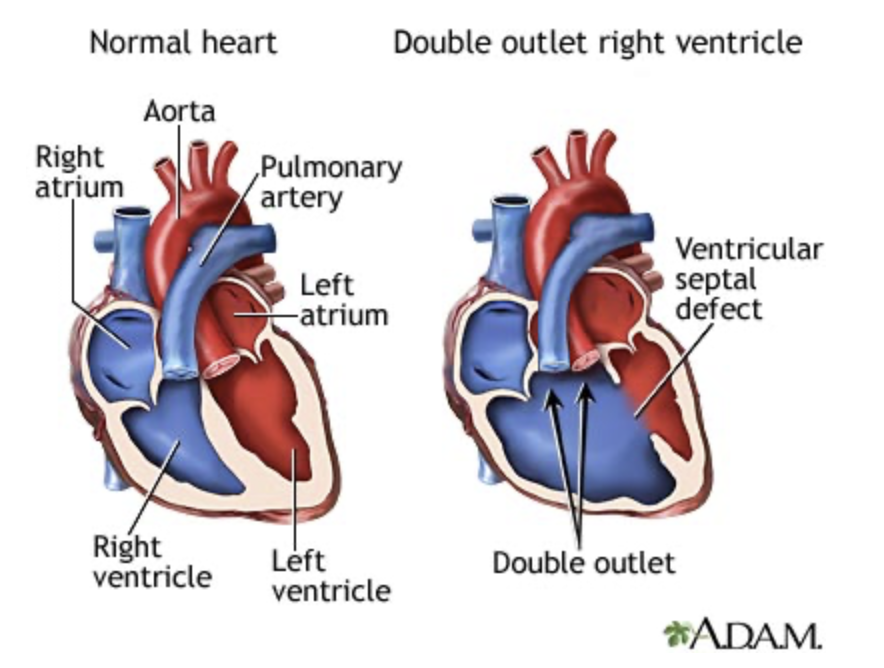
\includegraphics[height=6cm]{figures/intro/DORV_and_normal_schematics.png}
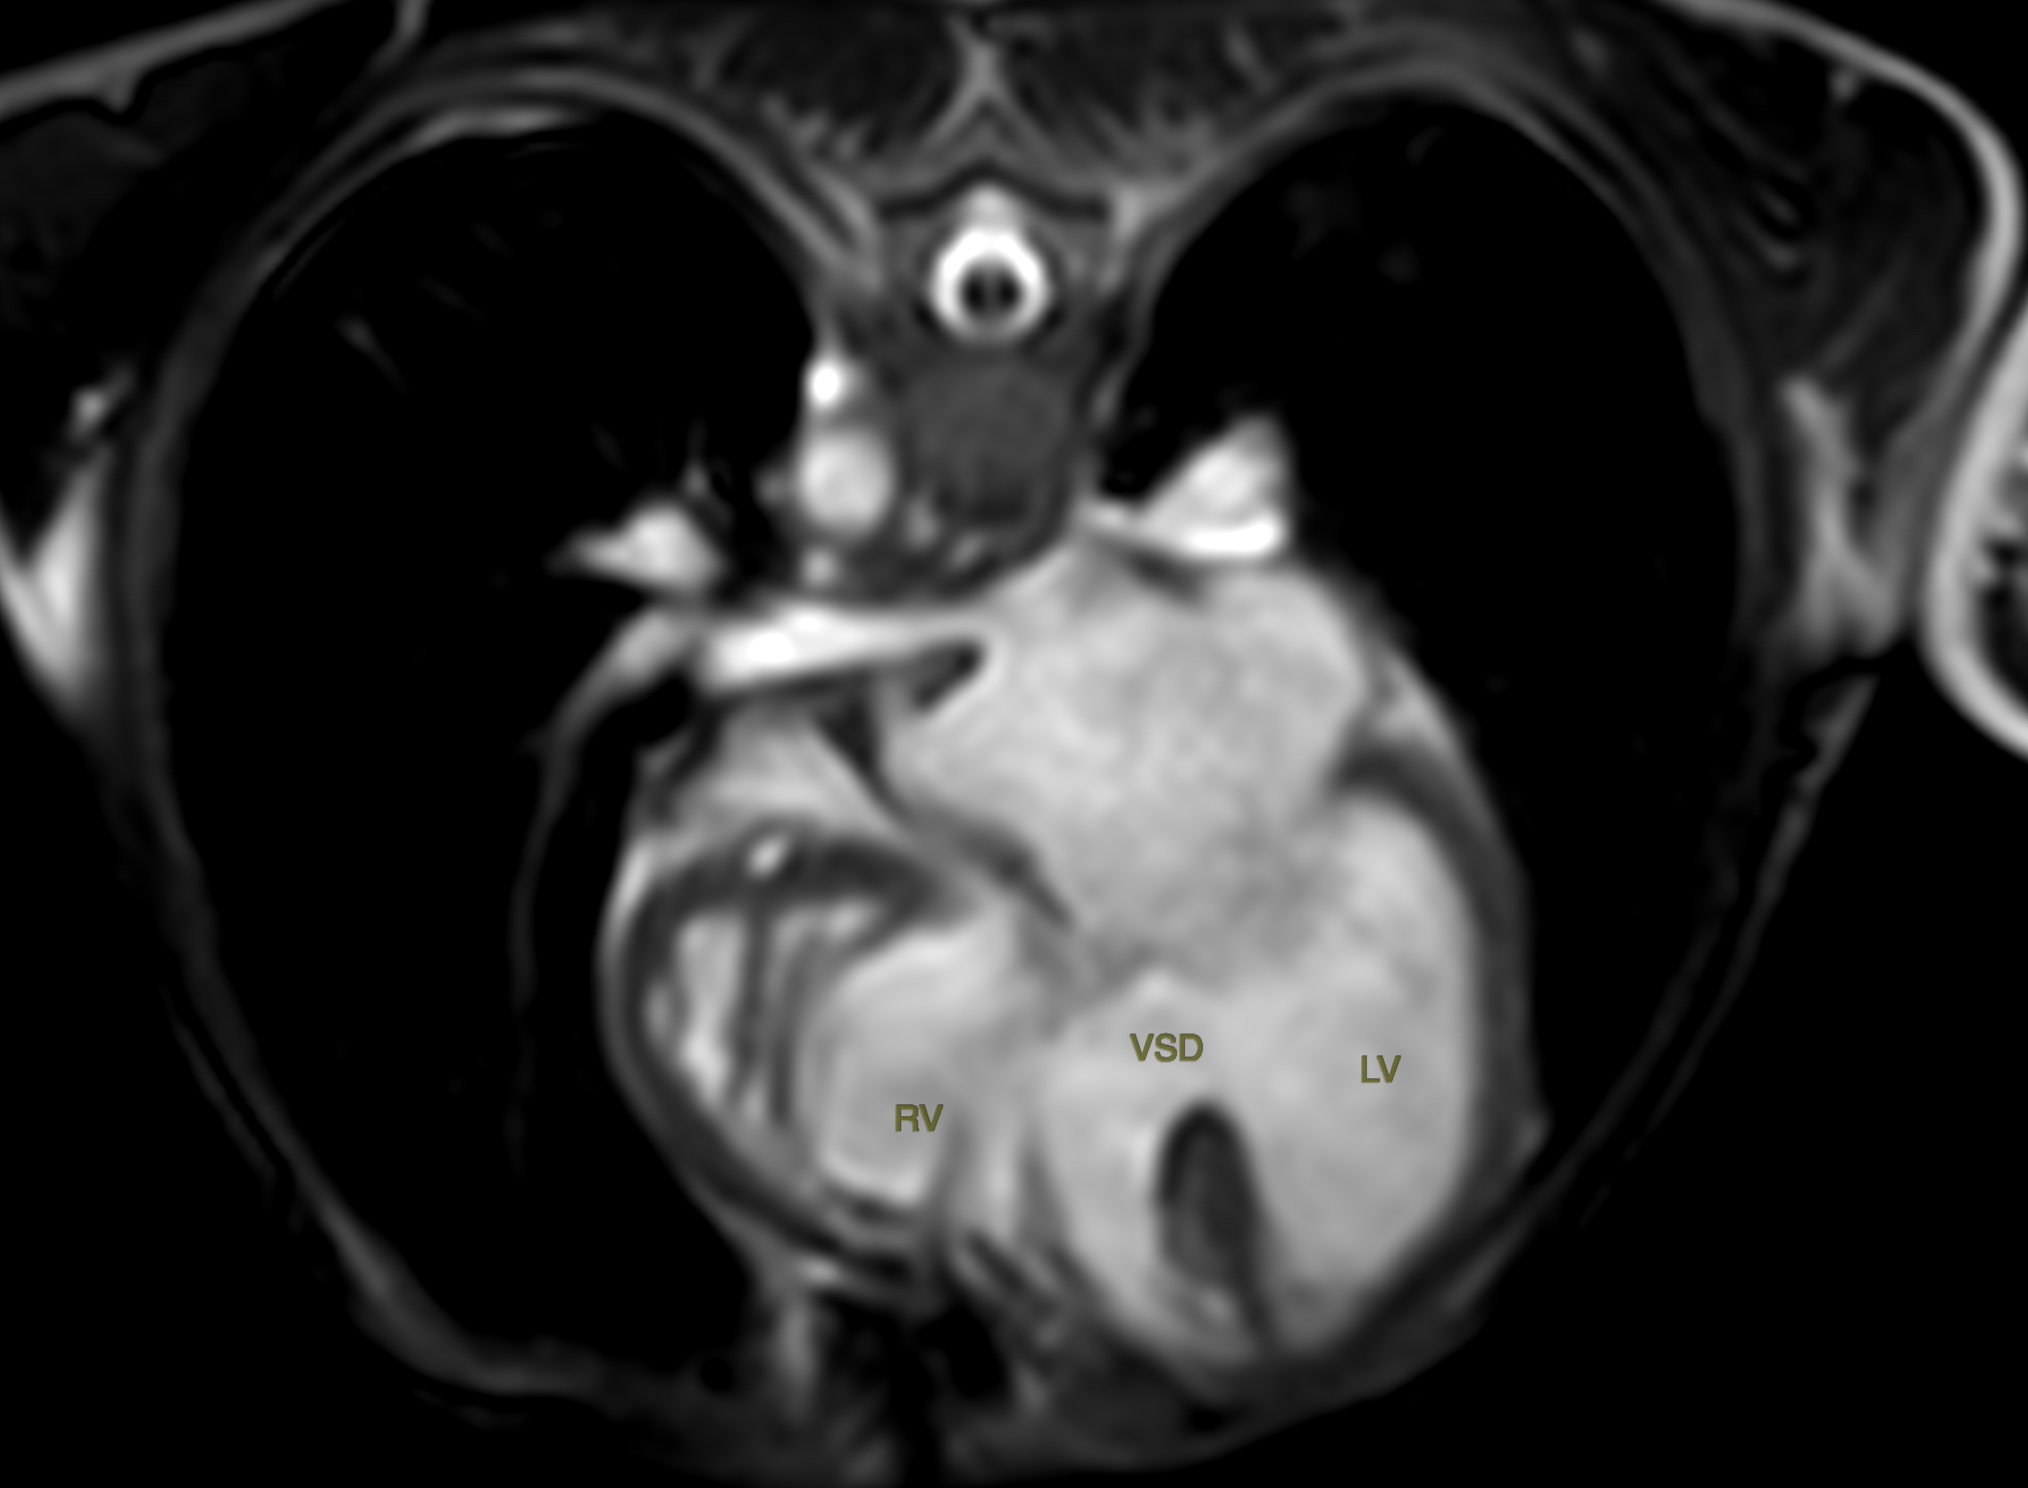
\includegraphics[height=6cm]{figures/intro/DORV06_4ch.jpg}
    \caption{\textbf{Illustration of a heart presenting double-outlet right ventricle (DORV), from A.D.A.M
Interactive Anatomy (left), and and MR image (right).
    % and simulating waveforms confronted with the measured data. 
    }} 
    \label{fig:intro_DORV}
    \vspace{-2pt}
\end{figure}

\textbf{Sub-aim 1a: Generation of Digital Twins from retrospective data of patients double-outlet right ventricle -- prototyping phase (Years 1 to 2).} 
We will employ the biomechanical heart model of a reduced geometry and kinematics\cite{caruel13}. This model was previously used in our clinical research projects\cite{ruijsink20,le_gall_monitoring_2020,gusseva23,gusseva25}. Ventricular geometry and kinematics are reduced to a sphere with inner radius $R$ and wall thickness $d$ (Figure \ref{fig:schematics}). Constitutive material laws that provide myocardial passive and active properties are preserved as in the full 3D heart model. In particular, myocardial passive stiffness is given by visco-elastic constitutive law; myocardial contractility is modeled within the A. F. Huxley sliding filament theory framework where mechano-chemical coupling of actin-myosin unit produces an active contraction of the sarcomere\cite{caruel13}. The model has been recently implemented as a Python library PhysioBlocks (distributed as an opensource software under the LGPL license), see 
\texttt{https://gitlab.inria.fr/physioblocks/physioblocks}.  

This library allows to create a cardiovascular model by assembling pre-defined blocks, e.g., actively contracting chamber; inflow and outflow valves (modeled as diodes, which incorporates a possibility of valve stenosis or regurgitation\cite{Gusseva_CJC_2021}), or inter-ventricular connection via ventricular septal defect (VSD); periphery circulation by 0D blocks of resistance/capacitance components (see example in Figures~\ref{fig:schematics_DORV_circuits} and \ref{fig:schematics}. The overall specific system consisting of a set of Blocks connected via a set of Nodes is called the ``PhysioBlocks Net''. 

We will pre-define the following vascular circuits and implement as the ``PhysioBlocks Nets''. These Nets will incorporate the majority of the patients with DORV (see Figure~\ref{fig:schematics_DORV_circuits}): 
\begin{enumerate}
\item Ventricular outflow into aorta and main pulmonary artery (MPA), with a pulmonary artery band (previously created, to reduce the risk of developing pulmonary hypertension); the pulmonary band is represented as a forward resistance of the pulmonary valve\cite{gusseva25}.
\item{Ventricular outflow into aorta (with pulmonary artery atresia); Glenn connection (superior vena cava to pulmonary artery junction) allows for partial oxygenation of blood}.
\item{Previous case, in addition, with developed significant aorto-pulmonary (AP) collaterals.}
\item{Ventricular outflow into aorta and main pulmonary artery (MPA), with a pulmonary artery band, and with the Glenn connection}.
\end{enumerate}

\begin{figure}%[t!]
    \centering
\subfigure[DORV to aorta and MPA]{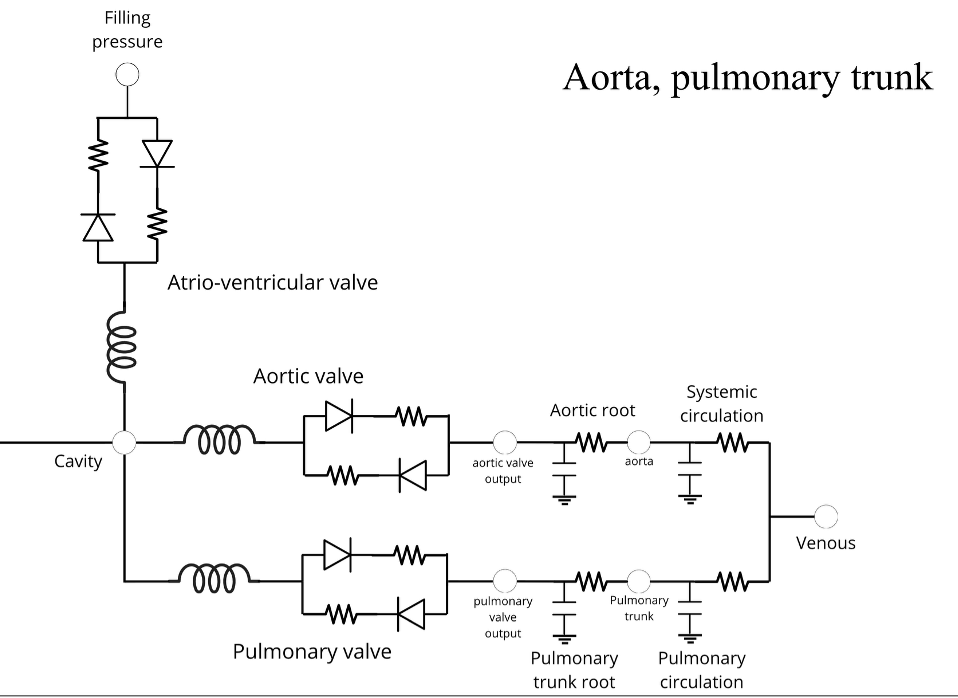
\includegraphics[width=0.49\columnwidth]{figures/schematics/circuits/circuit1.png}}    
\subfigure[DORV to aorta, with Glenn connection]{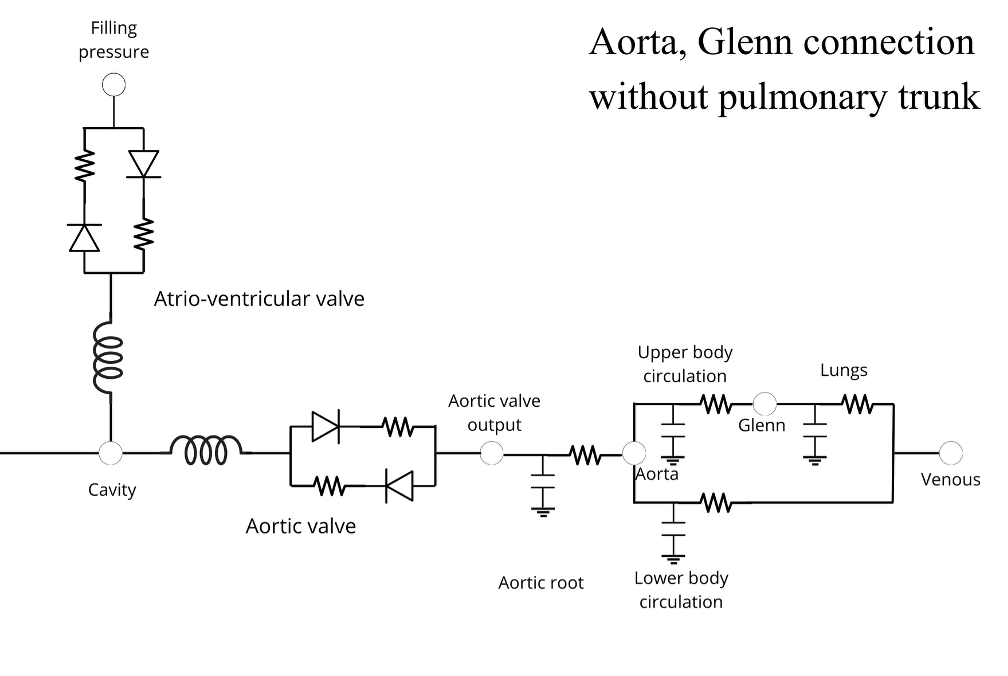
\includegraphics[width=0.49\columnwidth]{figures/schematics/circuits/circuit2.png}}   
\subfigure[DORV to aorta, with Glenn connection and AP collaterals]{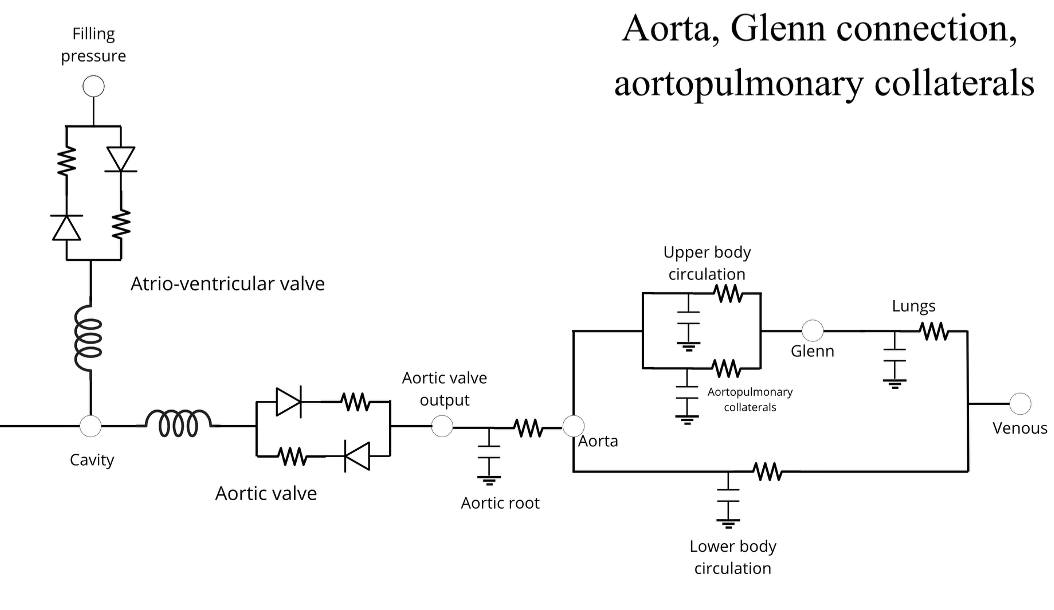
\includegraphics[width=0.49\columnwidth]{figures/schematics/circuits/circuit3.png}}   
\subfigure[DORV to aorta, MPA, with Glenn connection]{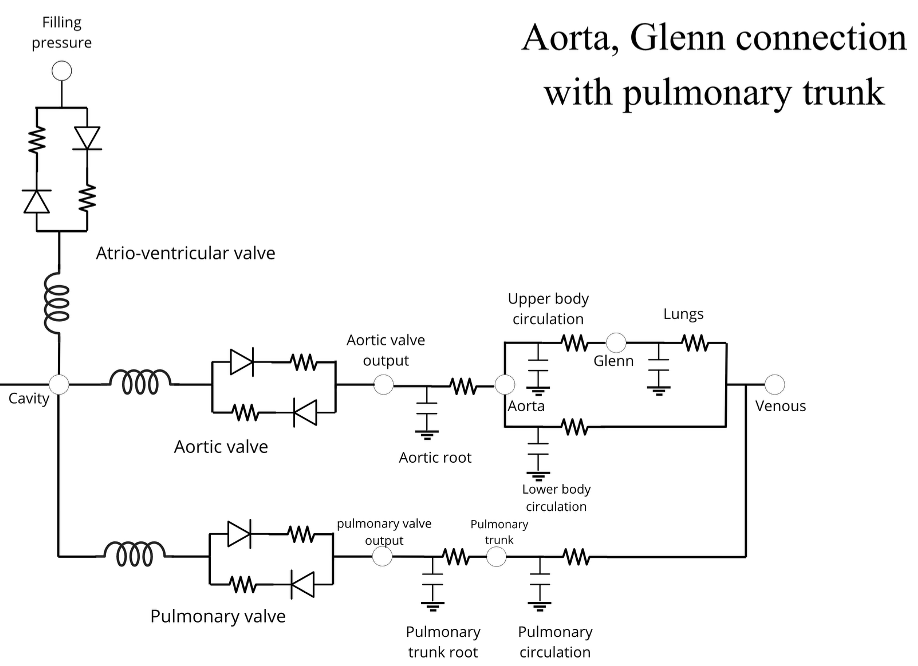
\includegraphics[width=0.49\columnwidth]{figures/schematics/circuits/circuit4.png}}   
    \caption{\textbf{Typical circulation configurations in the patients with double-outlet right ventricle (DORV) prior to BiV repair.} MPA, main pulmonary artery; AP, aorto-pulmonary.  \textcolor{red}{TO DO: replace the subfigures by nice/finalized schemes.}} 
    \label{fig:schematics_DORV_circuits}
    \vspace{-2pt}
\end{figure}


As for the contracting chambers for the patients with DORV, we will consider two configurations:
\begin{enumerate}
\item A single ventricle, incorporating both LV and RV, while neglecting the interventricular septum (adequate for the hearts with a large VSD, which is not restricting the flow between the two ventricles).
\item RV and a borderline-size LV will be represented by two ventricle blocks, connected via a VSD of a resistance creating the LV-to-RV pressure difference as observed in the pressurue data). This  configuration with an increased complexity will be used for smaller-sized VSD, restricting the LV-to-RV flow. 
 \end{enumerate}

%the implementation that will be used in this project.  



%Globally, the ventricular cavity pressure and volume are an output of the model. The heart model is coupled with inlet and outlet valves that are described by a system of diodes to control an inflow from the atrioventricular (AV) valve and an outflow through the ventricular outflow tract (VOT) with corresponding forward and backward AV/VOT valve resistances, $R_{for}^{(AV/VOT)}$  and $R_{back}^{(AV/VOT)}$\cite{gusseva21}. The circulation system will be extended to incorporate the specificity of the individual patients (such as, e.g., the band of main pulmonary artery\cite{gusseva25} or Glenn connection\cite{aramburu2024_closedLoopFontan}) by a specific implementation in the PhysioBlocks library (see example of a Glenn connection in Figure \ref{fig:schematics}).

%This will allow the flexibility of adjusting the connections in silico as per the planned BiV repair. 
\textbf{Model calibration at baseline}
During iCMR procedure, the following data are acquired: cine MRI (providing ventricular end-diastolic and end-systolic volumes, EDV, ESV and myocardial mass); flow in large-vessel (specific to the actual circulation; it typically incorporates flow measurements in: ascending and descending aorta; main, left and right pulmonary artery; superior and inferior vena cava); pressure waveform in the heart chambers and in large vessels (corresponding to the flow measurements). 

The model will be turned into a patient-specific mode by applying the  sequential calibration procedure\cite{ruijsink20,gusseva21}. Windkessel model parameters (resistances and capacitances in the circuit), are adjusted to match the measured pressures while imposing the measured inflow.  Then, in the ventricular cavity model the wall thickness and sphere radius is prescribed from cine MRI mass and EDV measurements. Ventricular preload is imposed from the measured ventricular EDP. Passive myocardial stiffness will be adjusted to match measured EDV under the imposed preload. Myocardial contractility is calibrated according to the measured stroke volume and end-systolic pressure in the ventricle. 
The example patient specific simulations are presented in Figure~\ref{fig:schematics}.

\begin{figure}%[t!]
    \centering
%    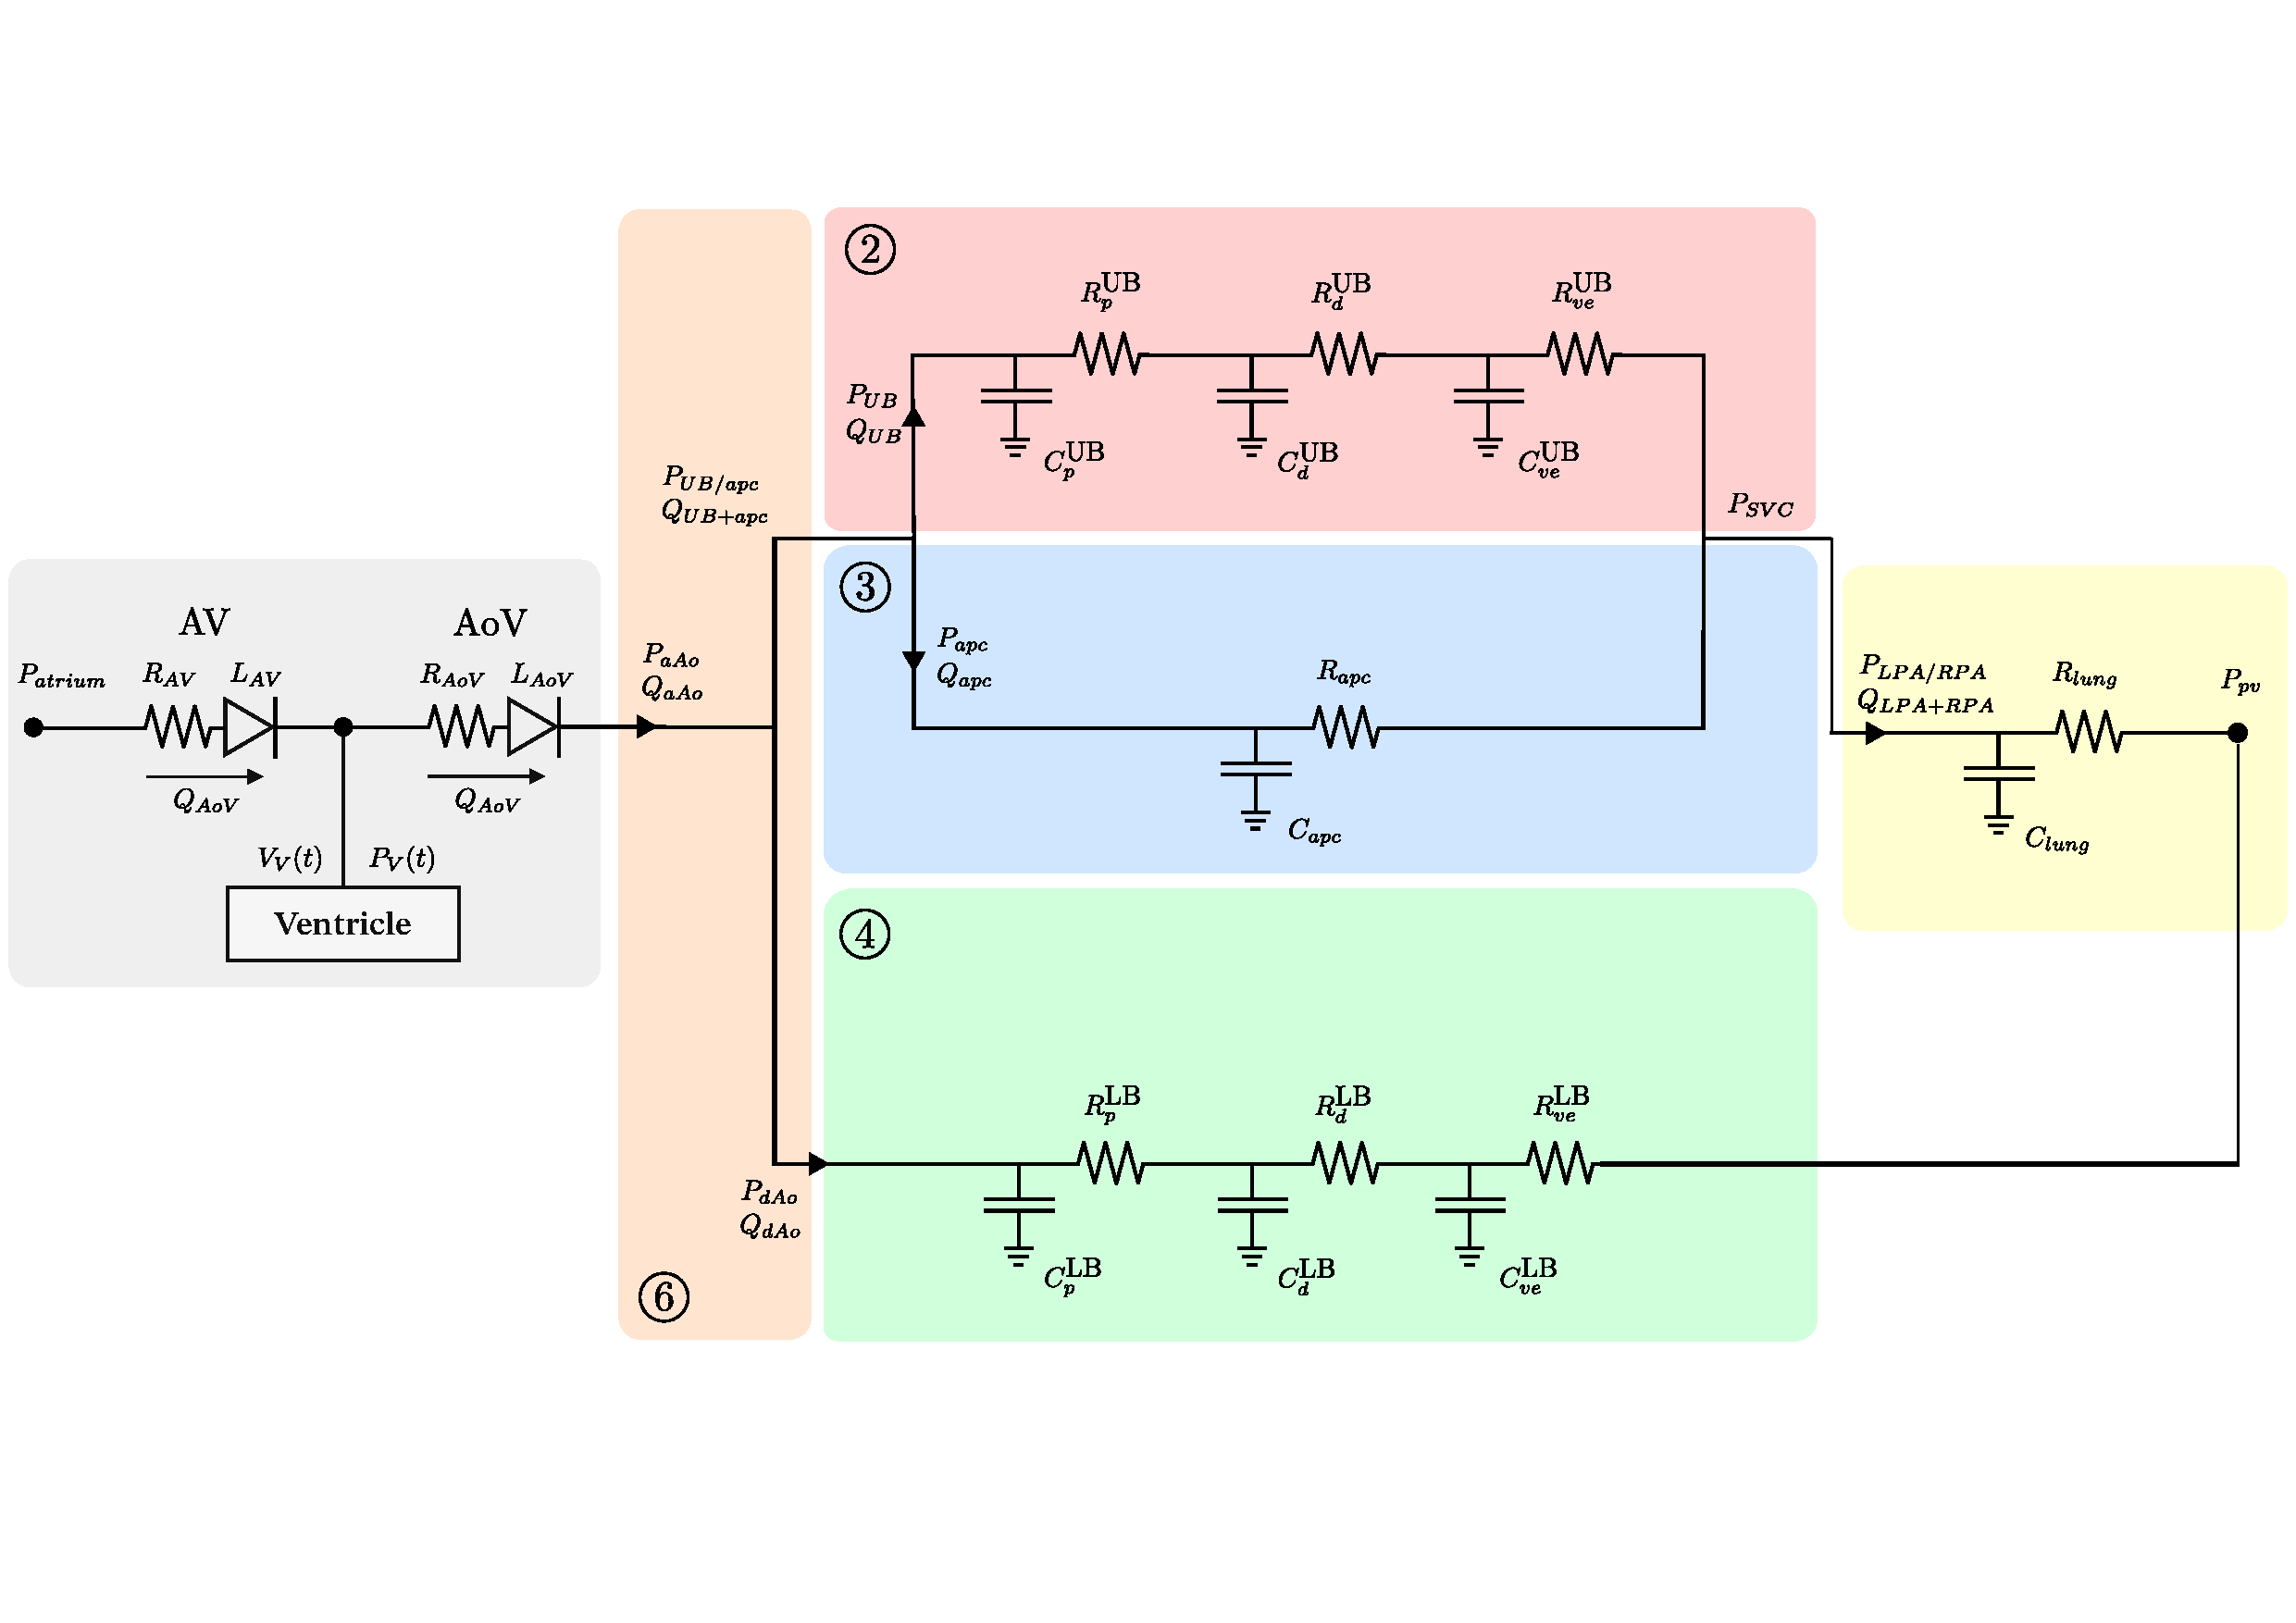
\includegraphics[width=1\columnwidth]{figures/schematics/circuit_DORVwithGlenn.pdf}
    %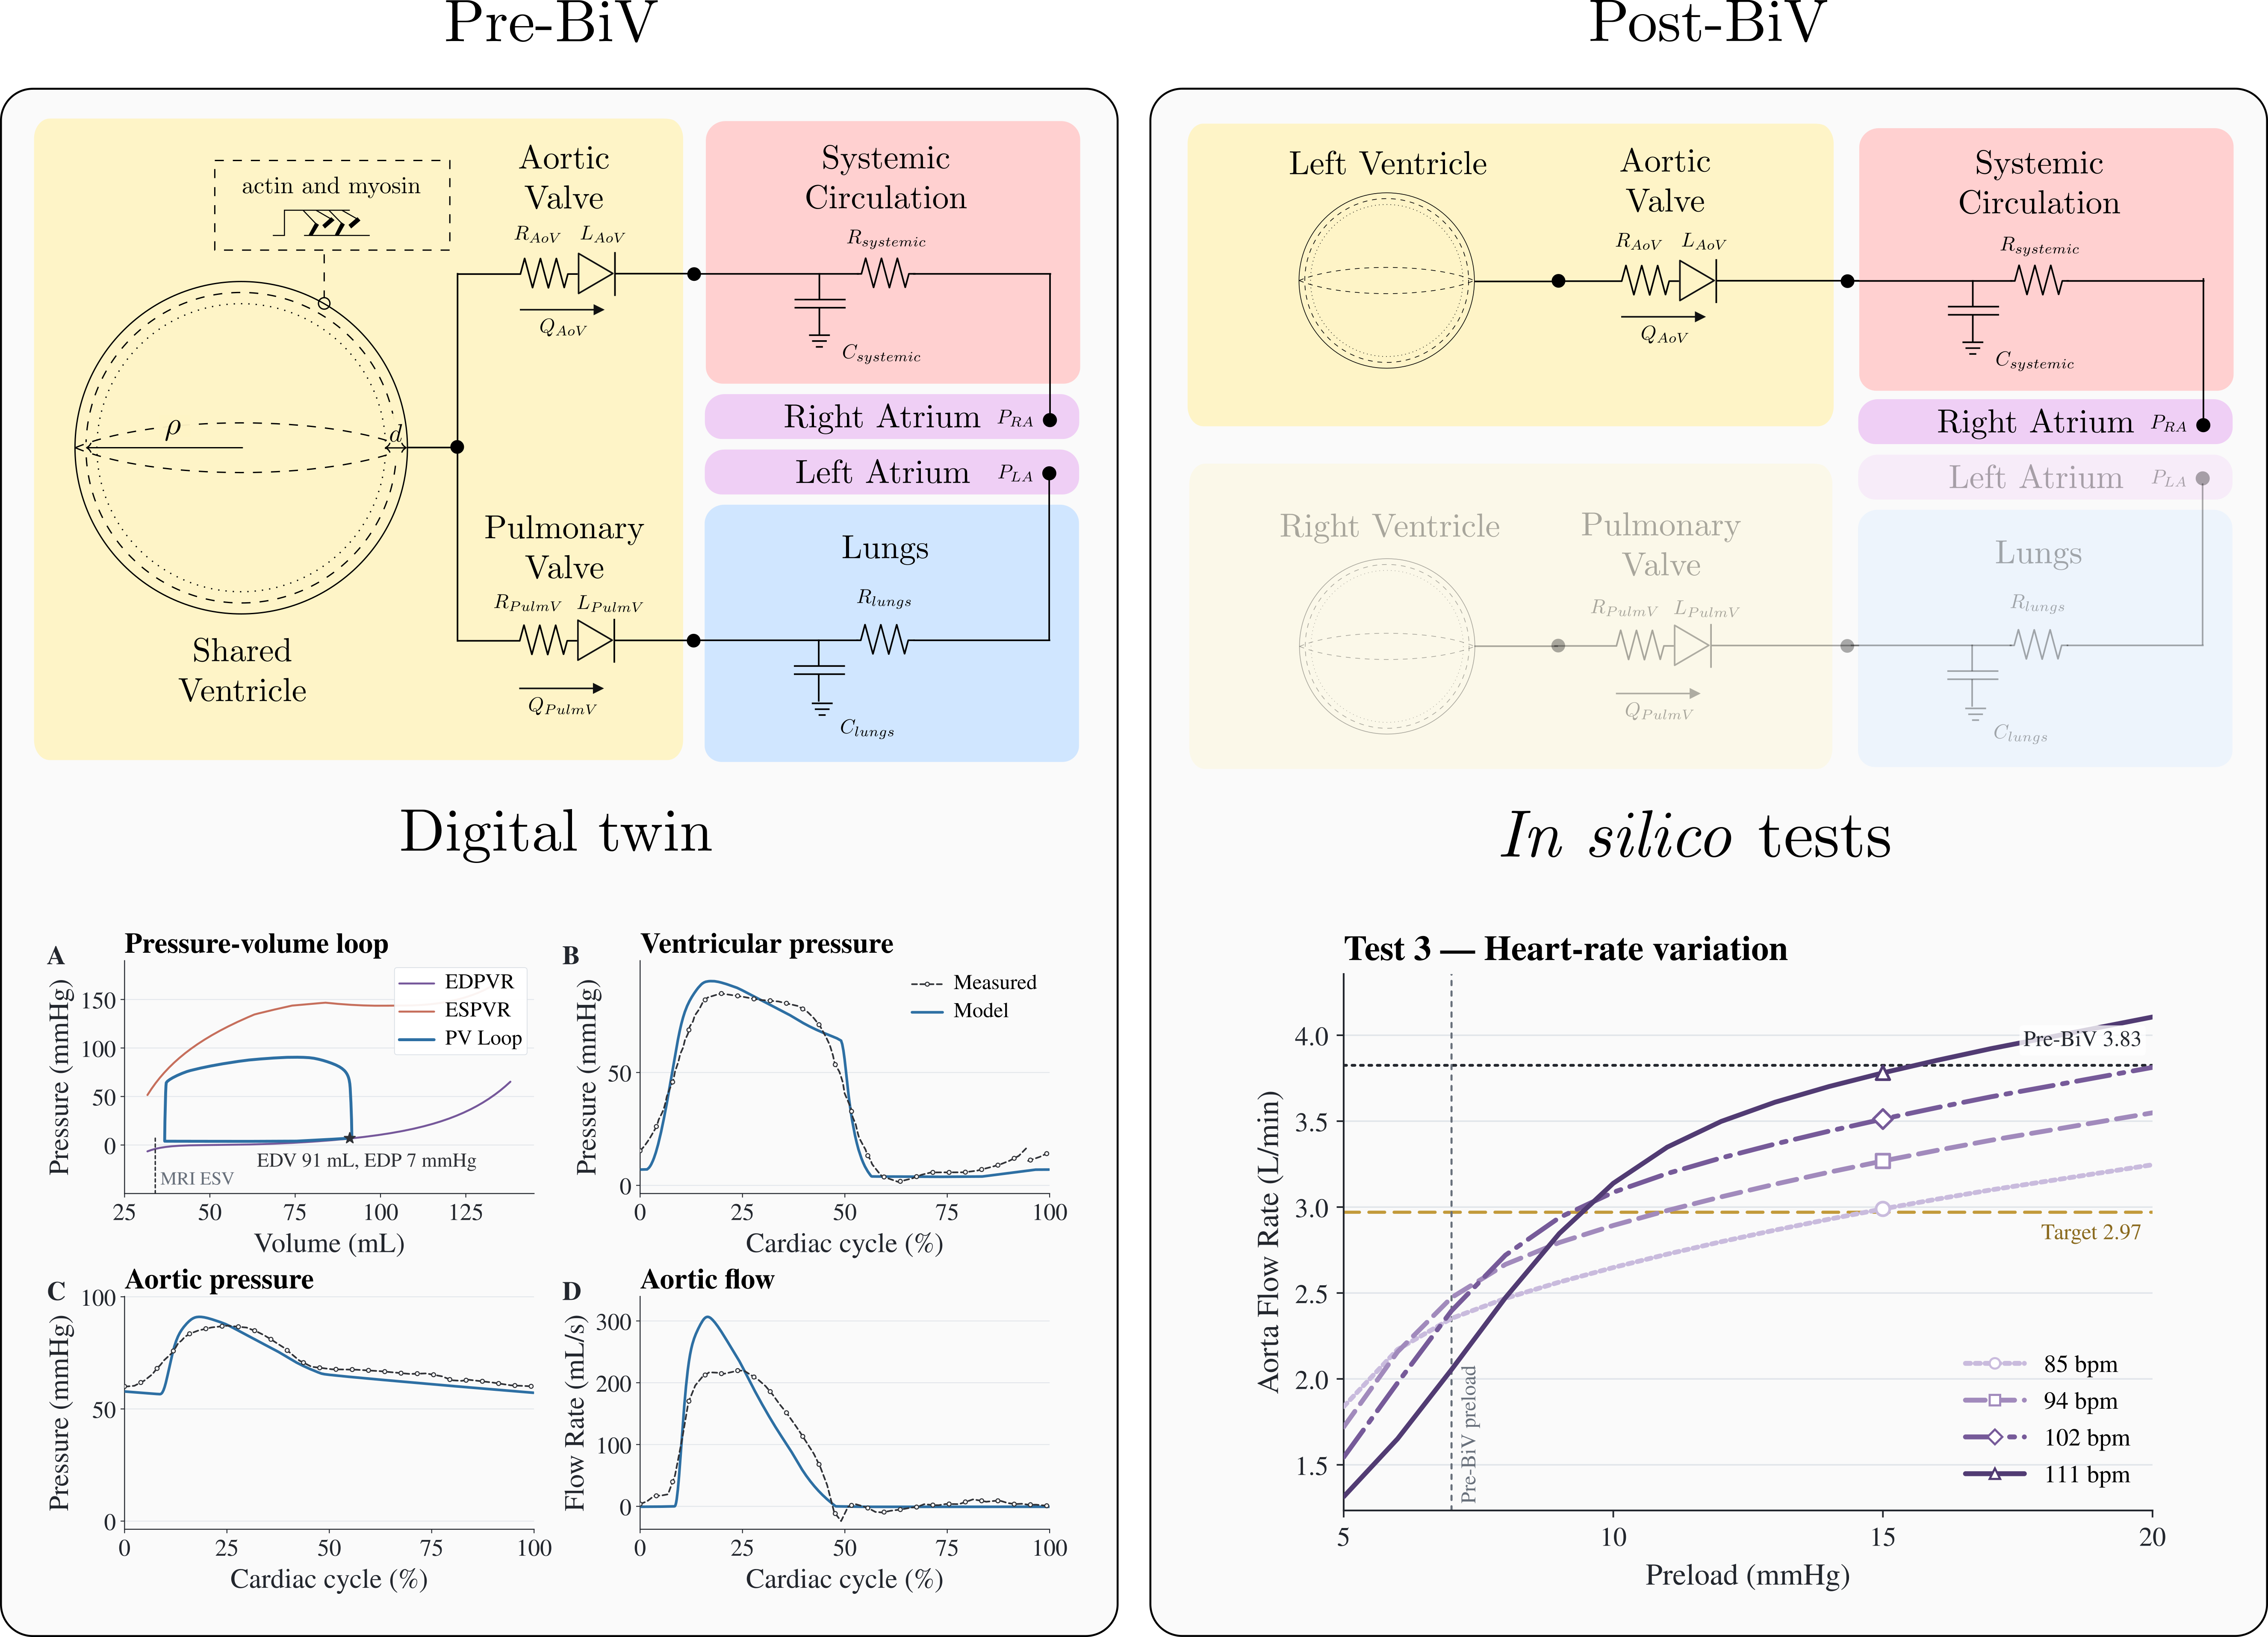
\includegraphics[width=1\columnwidth]{figures/schematics/DORV_BiV_model.png}
    \includegraphics[width=0.51\columnwidth]{figures/schematics/DORV_pre_biv.jpg}
    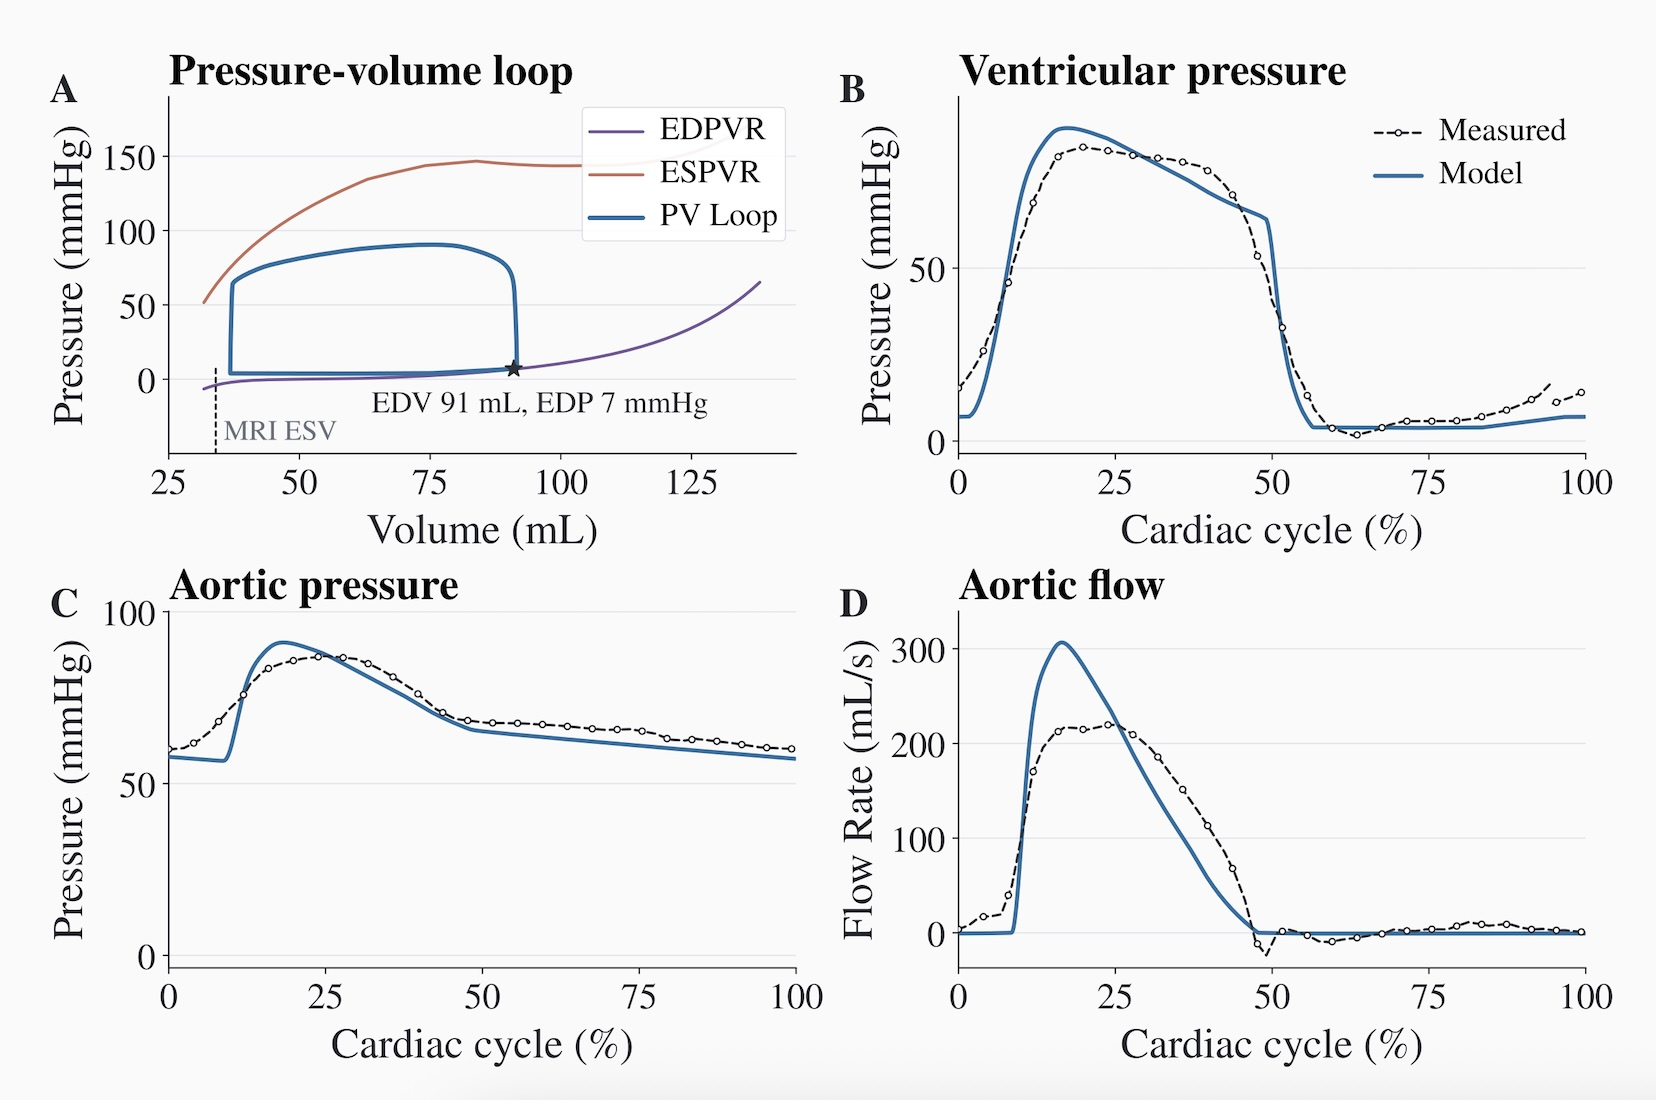
\includegraphics[width=0.48\columnwidth]{figures/simulations/DORV/DigitalTwin_DORV.jpg }    
    \caption{\textbf{Model schematics for an example patient with double-outlet right ventricle and the functional indicator of the created Digital Twin.
    % and simulating waveforms confronted with the measured data. 
    }} 
    \label{fig:schematics}
    \vspace{-2pt}
\end{figure}


\textbf{Model re-calibration during iCMR.} 
%During the iCMR procedure, a complete dataset of 
The changes of physiology, which can arise during the iCMR procedure,  -- induced, e.g.,  by the need of a vasoactive drug administration -- will provide a limited dataset consisting of the flow in ascending aorta together with the aortic pressure. The baseline model will be adapted using the methods from our previous works related to model-augmented cardiovascular physiology during general anesthesia\cite{le_gall_monitoring_2020} and of automated parameter estimation (sequential data assimilation into the biomechanical model using Kalman-like filtering)\cite{chabiniok12}. 

\textbf{Modeling outcomes augmenting the iCMR data}
The Digital Twin will act as ``biophysical filter'', which will reduce the uncertainty in the iCMR data\cite{gusseva2023_timeSynch_JMRI,gusseva_AJPHeartCirc_2025} and provide additional quantities of clinical interest, not directly visible in the data. Namely, the iCMR data analysis will be augmented by:  ventricular pressure-volume (PV) loops of a high quality\cite{gusseva_AJPHeartCirc_2025}; ventricular elastance\cite{legall19}; myocardial stiffness and the actual value of the contractility and resistances in the circuit\cite{ruijsink20,le_gall_monitoring_2020}.


\textbf{Sub-aim 1b: Digital Twin-augmented iCMR platform (Year 1-2)}
While the PhysioBlocks library (Sub-aim 1a) will be used 
for the prototyping and testing, a customized software adapted to the data (discrete values characterizing the anatomy of the ventricles, and pressure and flow waveform output of iCMR system) and embedding the models defined in Sub-aim 1a, will be developed in parallel. The experience of the Twynova with providing solutions for the ICU and general anesthesia setups (continuous waveforms of pressure and cardiac output, real-time adapting the predefined Digital Twins\cite{kimmig_FIMH2025})) will allow for a technical solution incorporating the specific data output of iCMR. The fast engine (acceleration factor around 10, in comparison to the PhysioBlocks prototyping), will be suitable for the actual automation of the creation of Digital Twins directly during the iCMR procedure. 

The intended product will contain a graphical user interface, which will allow the clinical experts to select the pre-defined models and their modification according to the individual patients, while providing the ``on-the-fly'' Digital-Twin-data augmentation.

\textbf{Sub-aim 1c: Extension of the study population to all patients considered for BiV repair (Year 3)}
The model defined in Sub-aim 1a will be generalized to all patients with borderline-size LV (not limited to the patients with DORV) and with borderline-size RV. In the latter group, we will consider the BiV repair (septated LV and RV, as previously delineated) and the so-called ``1.5-ventricle repair'' (smaller RV receiving venous return from the inferior body, while the upper body-venous return is connected to pulmonary arteries via the Glenn connection). 

\textbf{Sub-aim 1d: Extension of the study population to all patients considered for BiV repair (Year 4-5)}
The DT-augmented iCMR analysis will be performed  prospective patients undergoing iCMR exam prior to their BiV repair. 









\subsubsection{Aim 2}
The Digital Twins of patients undergoing BiV repair created in Aim 1 will be modified according to the planned surgery. The borderline-size ventricle will be connected to the systemic / pulmonary circulation, in the patients with borderline-size left, right ventricle, respectively. We will assume that the flow rate in systemic/pulmonary circulation is unchanged after the repair and that the morphology of the borderline-size ventricle is modified according to the septated ventricle. While the passive myocardial stiffness will be assumed to be unchanged from pre-BiV stage, the contractility (inotropy level), heart rate, ventricular preload (represented by LV EDP) and level of the atrio-ventricular valve insufficiency, will be varied in silico. The predicted non-favorable outcomes from BiV conversion will be defined by predicted heart rate higher than the upper normal range (for patient’s age); ventricular preload above 15 mmHg or need for ventricle contractility above the level prior to BiV conversion. 

Plots in Figure~\ref{fig:BiV_repair} demonstrate such in silico predictions when varying the LV preload, chronotropic and inotropic effects, suggesting a more complicated post-surgery course. Figure\ref{fig:DORV4} demonstrates a predicted favorable post-surgery course.  A result of pilot study with 6 patients with DORV is presented in Figure~\ref{fig:BiV_table}.

\begin{figure}%[t!]
    \centering
%    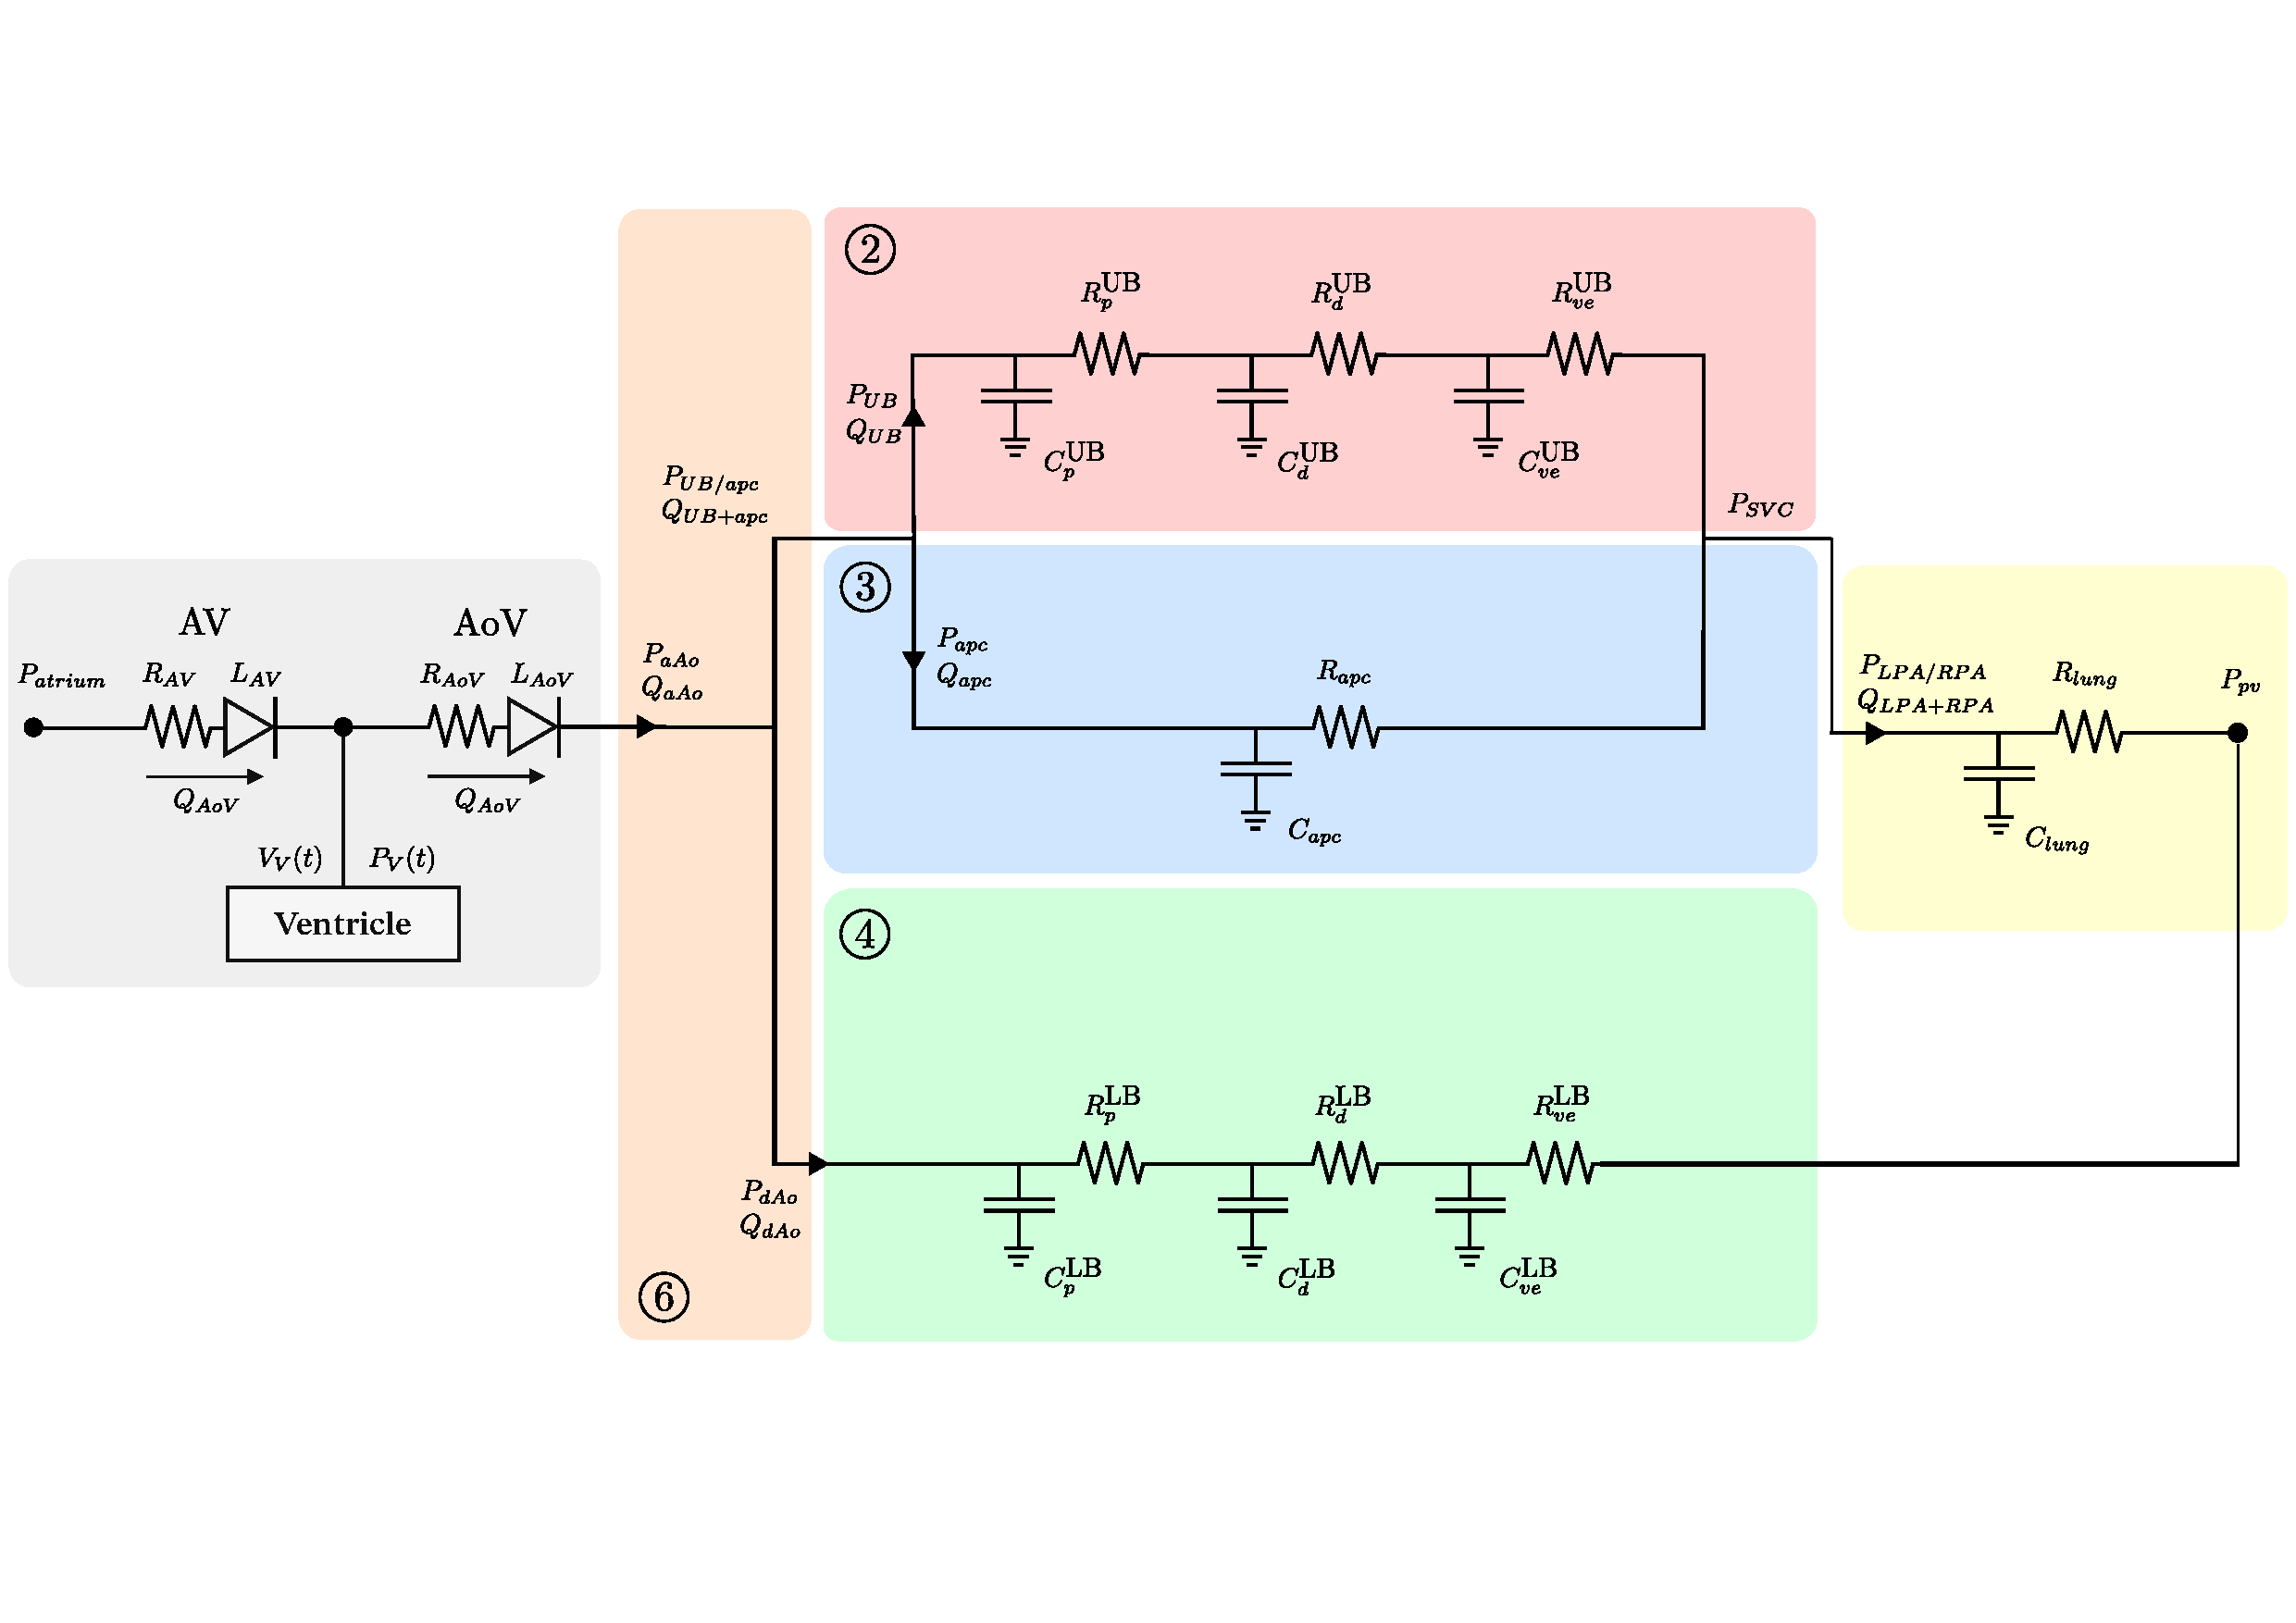
\includegraphics[width=1\columnwidth]{figures/schematics/circuit_DORVwithGlenn.pdf}
    %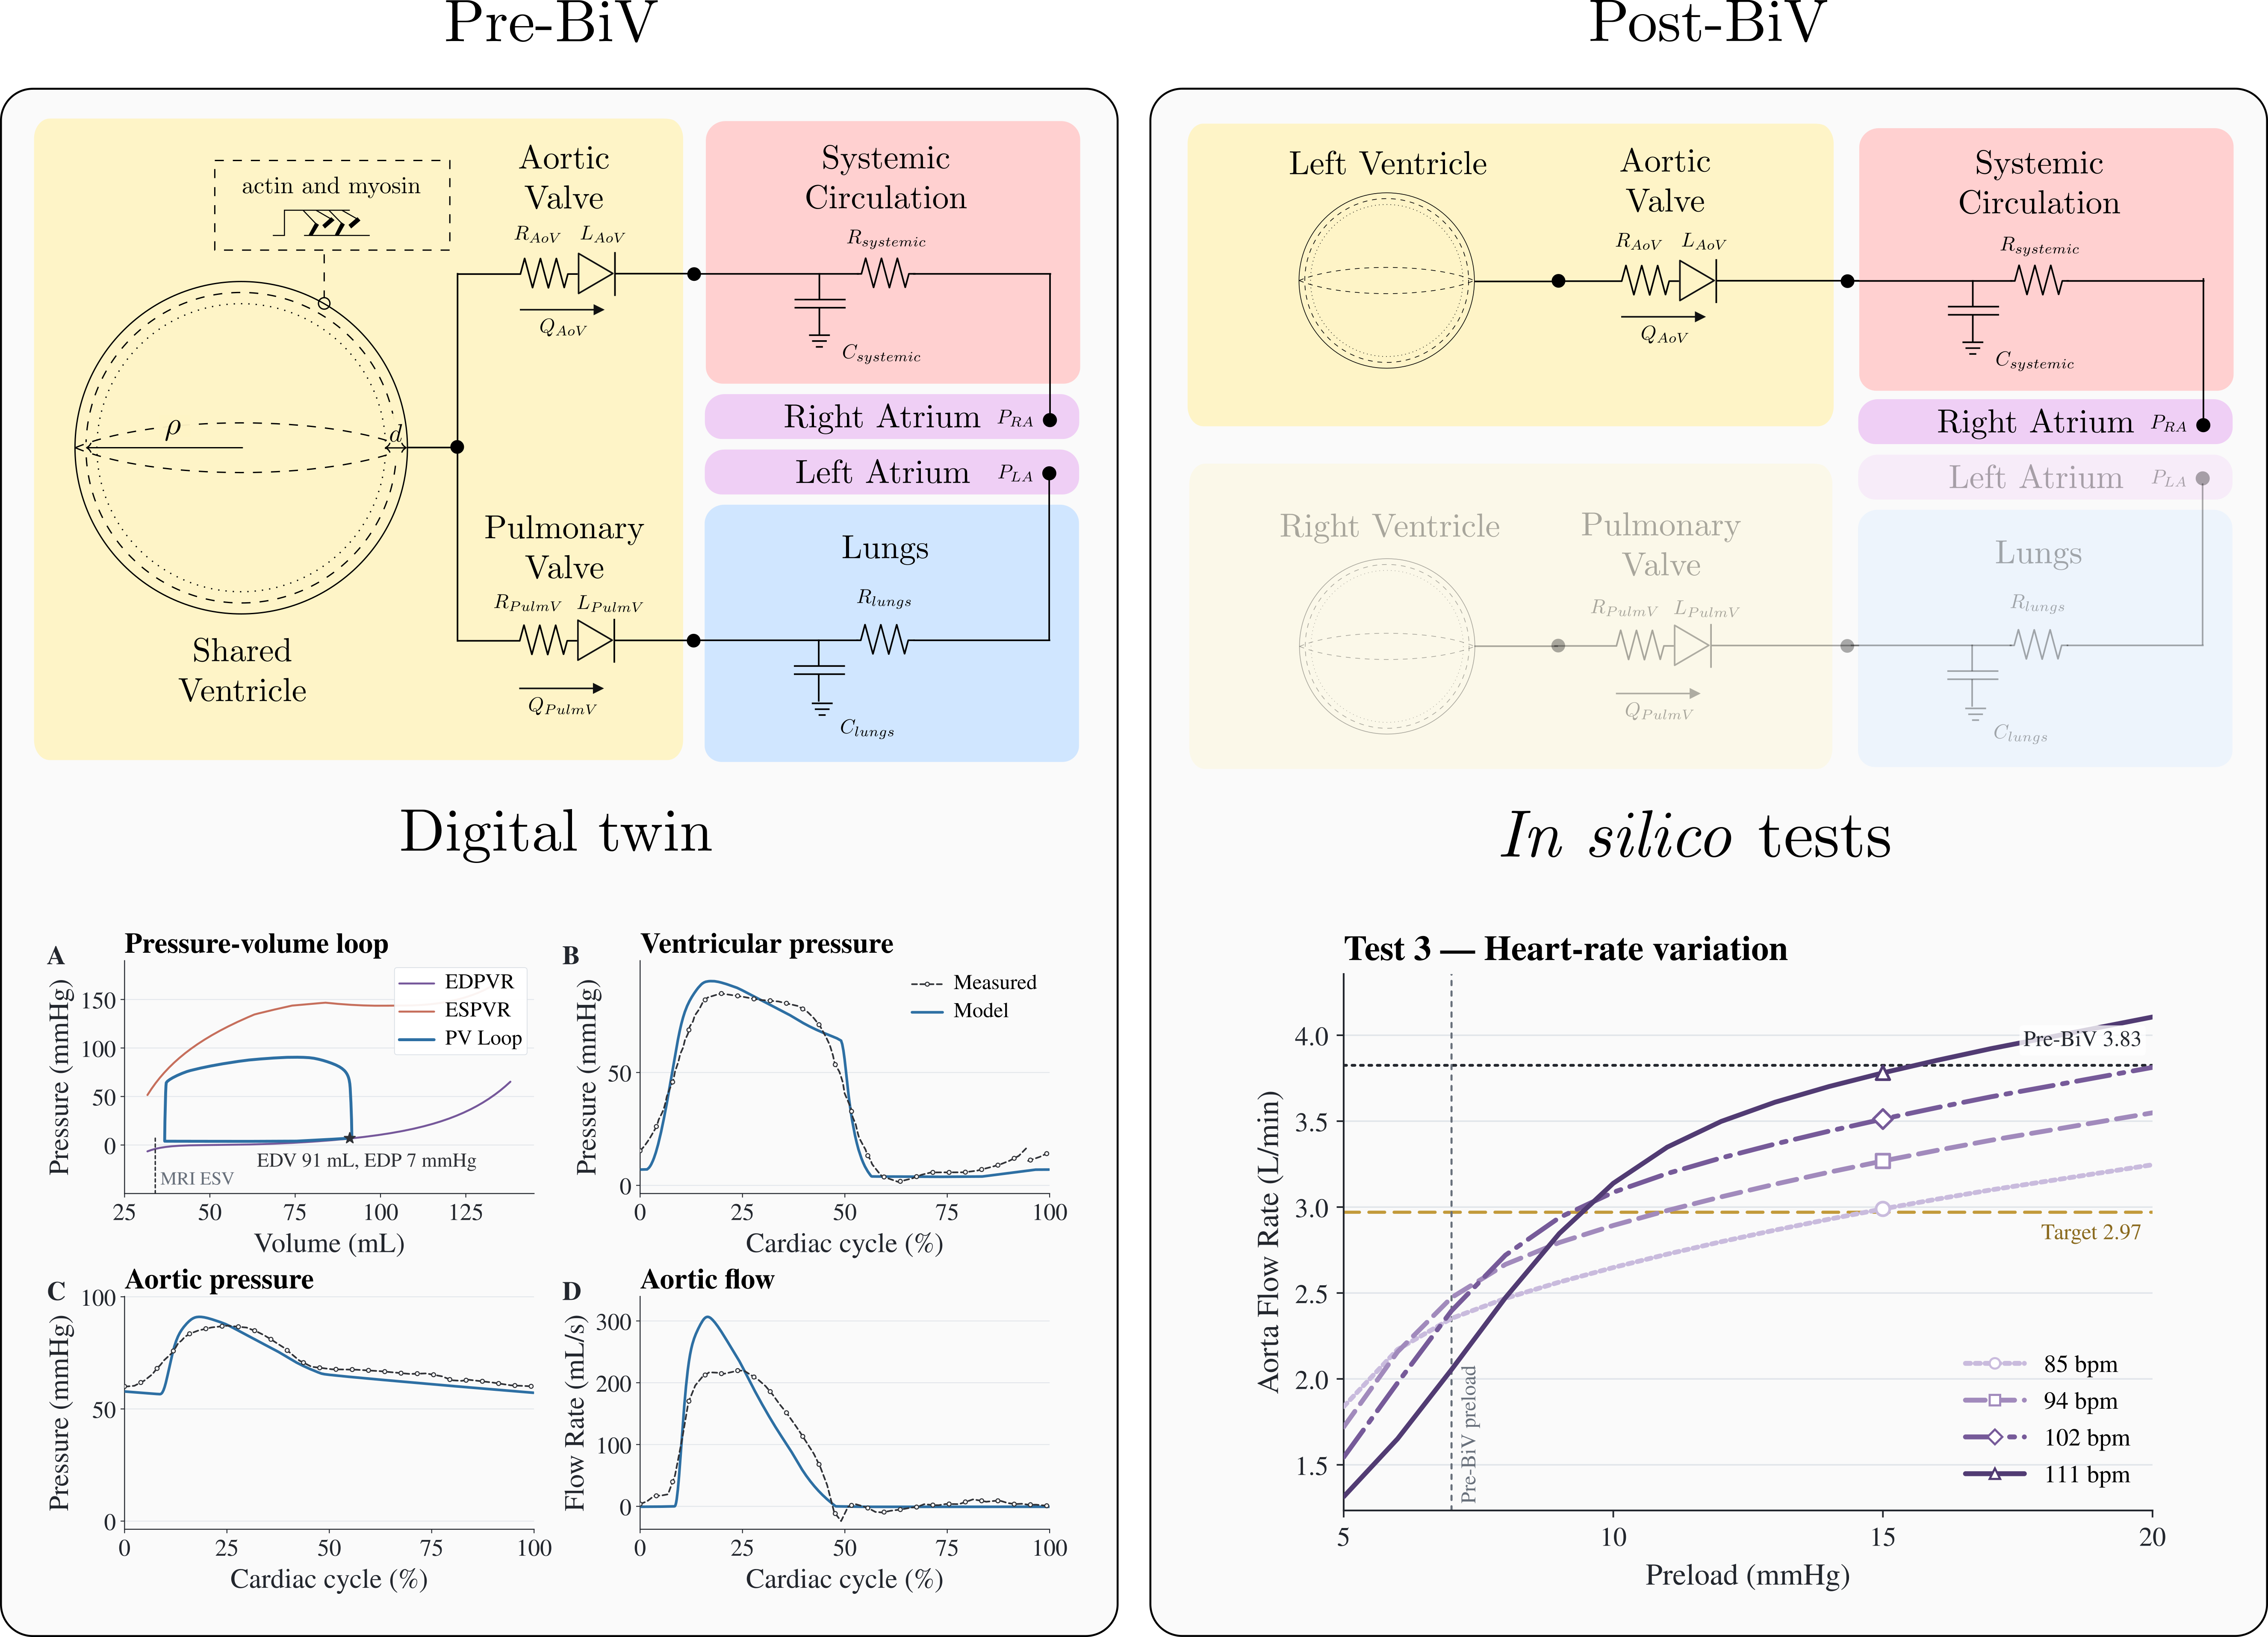
\includegraphics[width=1\columnwidth]{figures/schematics/DORV_BiV_model.png}
    \includegraphics[width=0.65\columnwidth]{figures/schematics/DORV_post_biv.jpg}    \\
    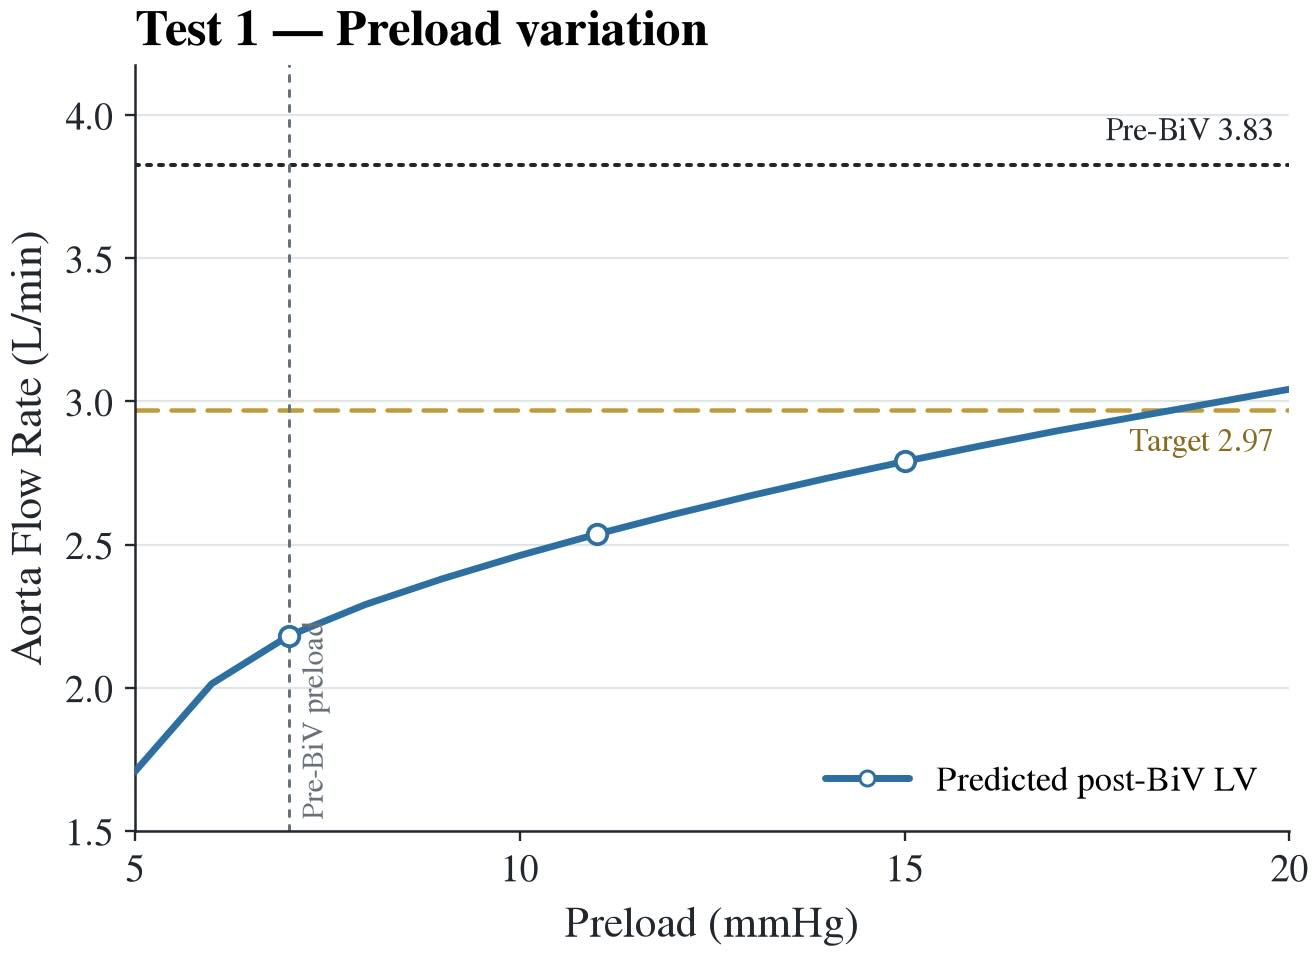
\includegraphics[width=0.49\columnwidth]{figures/simulations/DORV/test1_preload.jpg}
    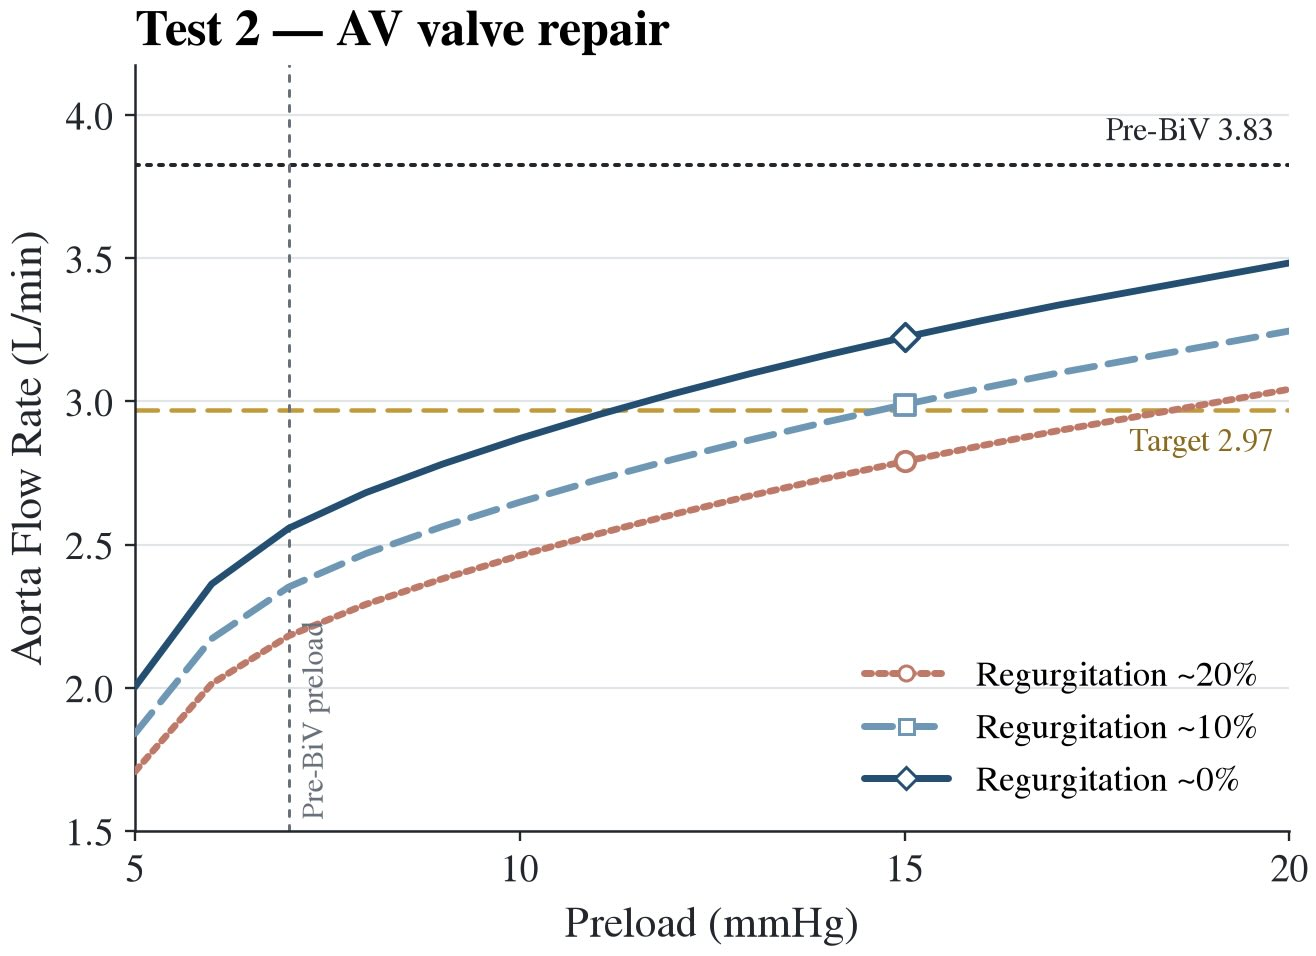
\includegraphics[width=0.49\columnwidth]{figures/simulations/DORV/test2_valve_repair.jpg}
    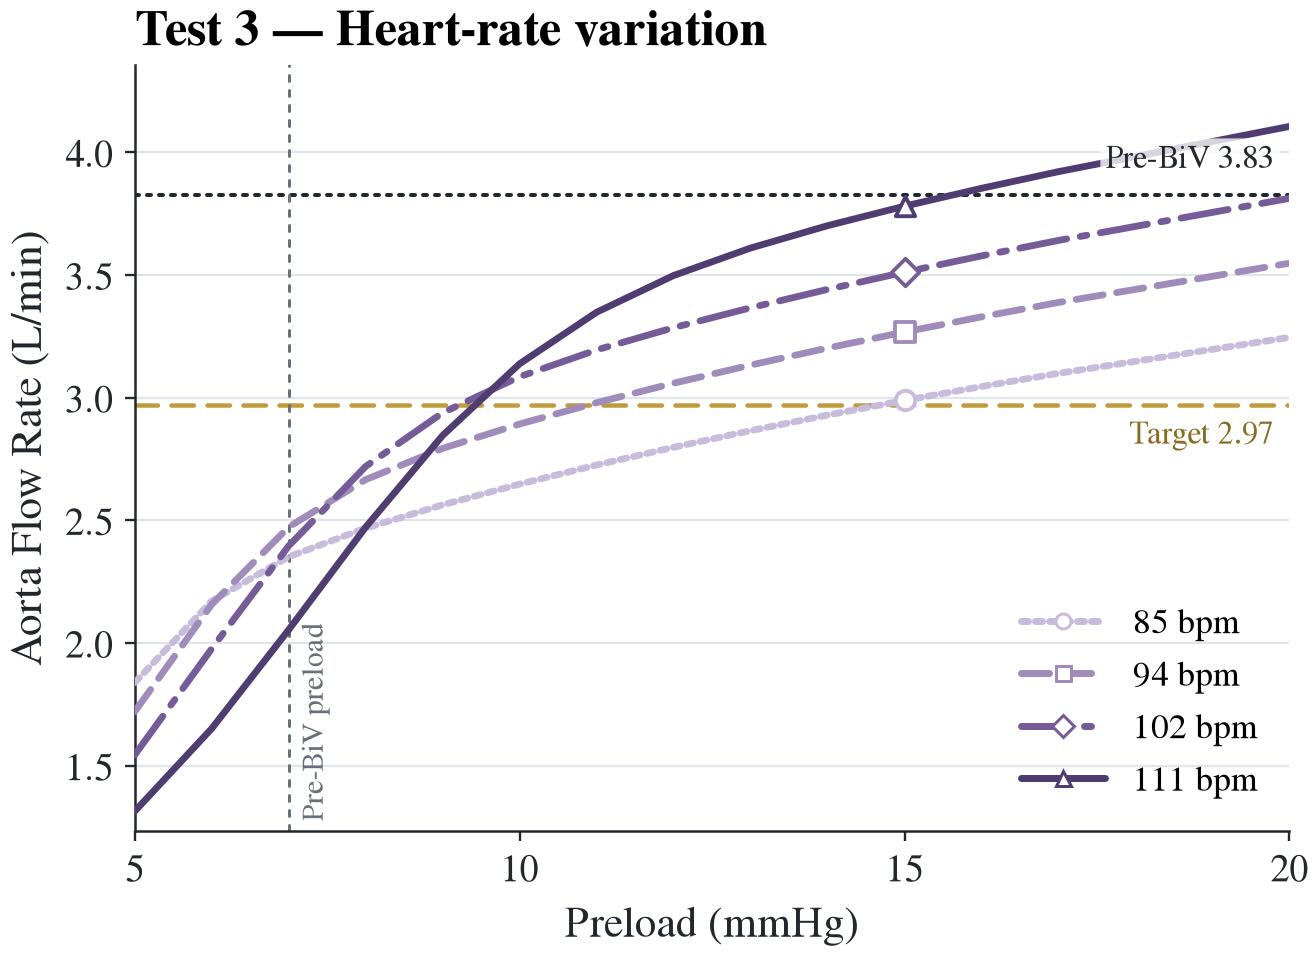
\includegraphics[width=0.49\columnwidth]{figures/simulations/DORV/test3_heart_rate.jpg}
    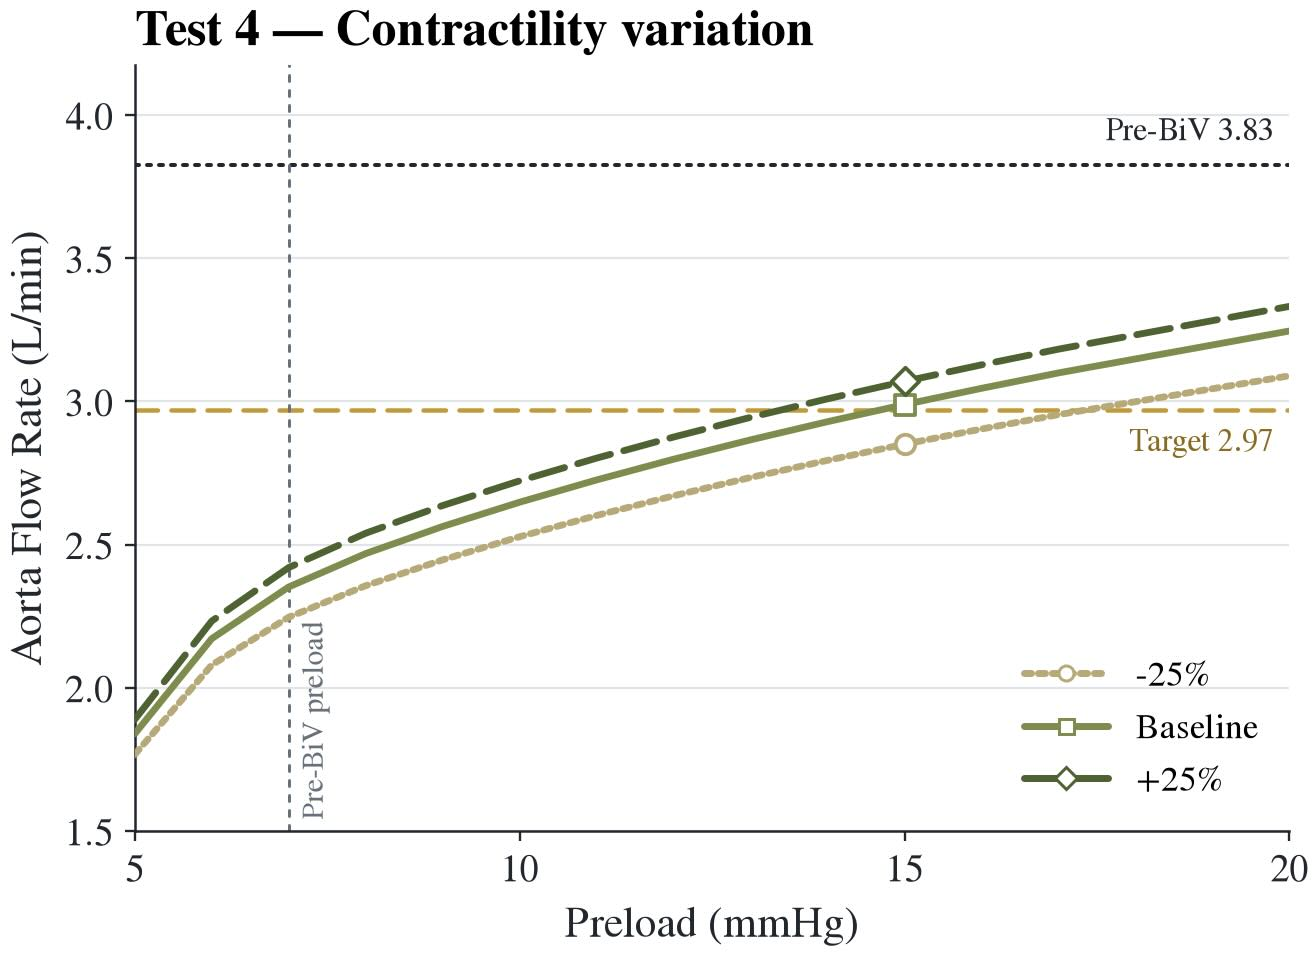
\includegraphics[width=0.49\columnwidth]{figures/simulations/DORV/test4_contractility.jpg}
        
    \caption{\textbf{{In silico} biventricular repair (left ventricular septation and connection with the systemic circulation) and prediction of the function of the ventricle.
    }} 
    \label{fig:BiV_repair}
    \vspace{-2pt}
\end{figure}

\begin{figure}%[t!]
    \centering
%    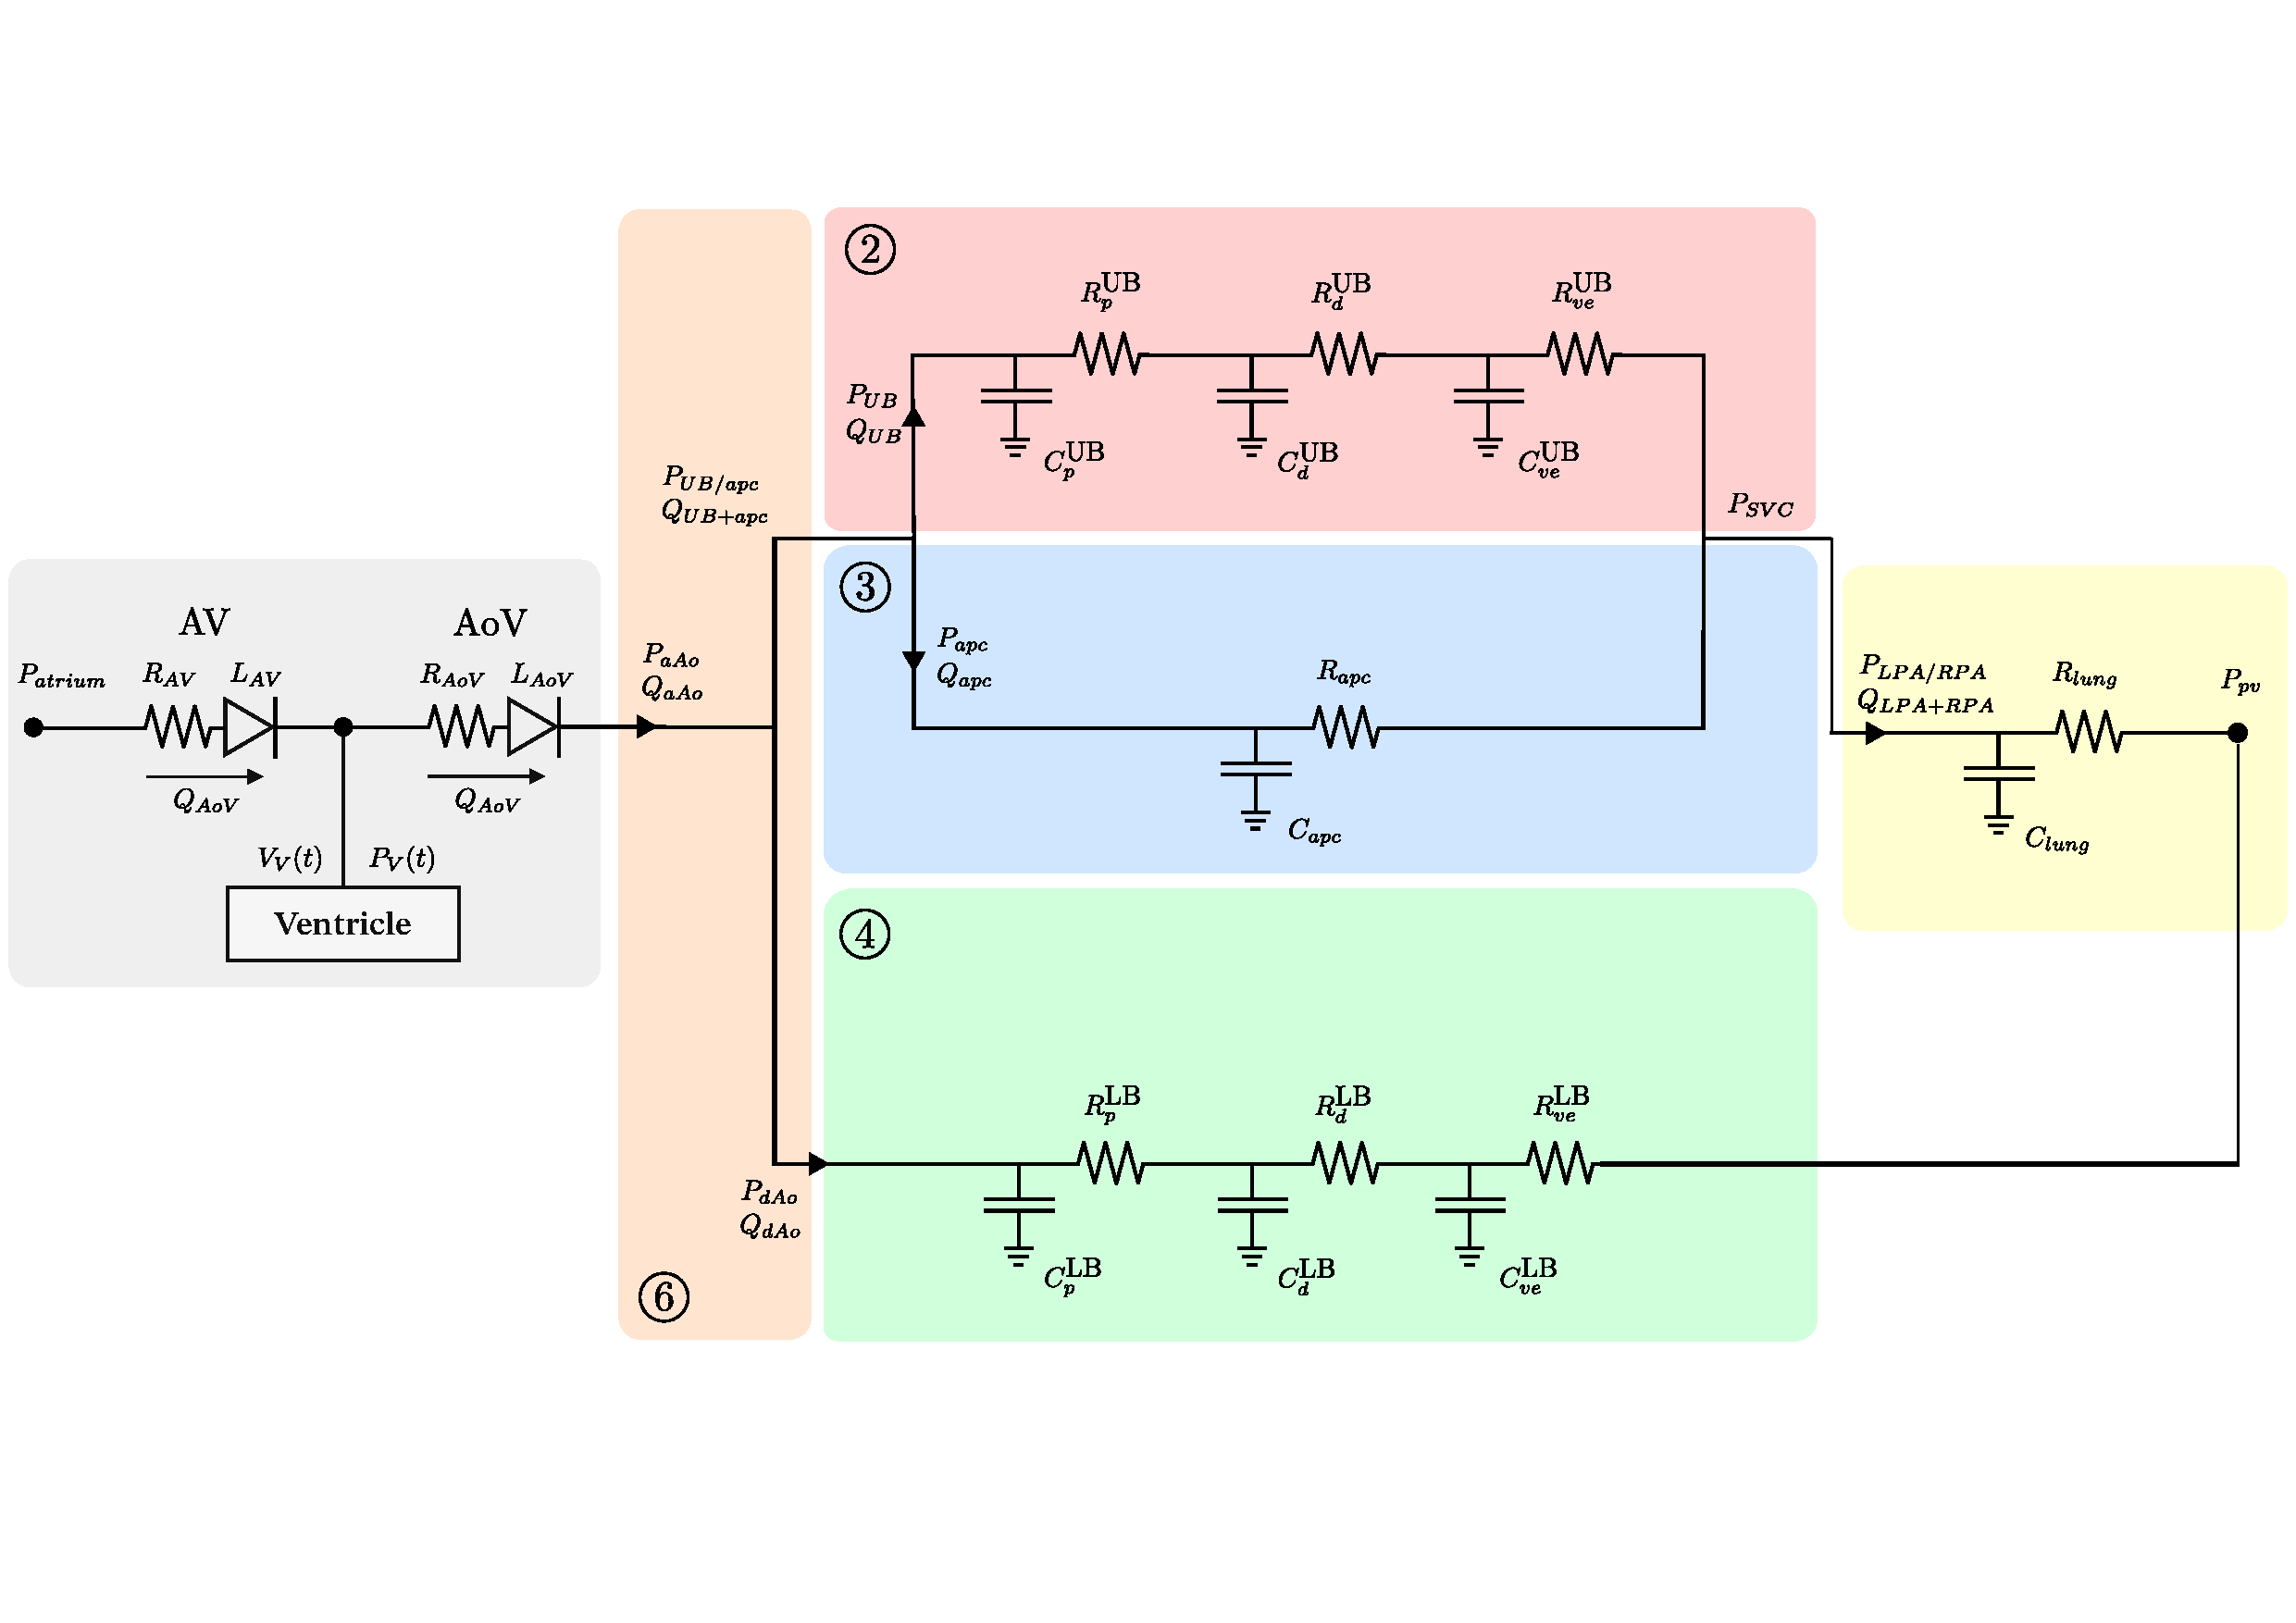
\includegraphics[width=1\columnwidth]{figures/schematics/circuit_DORVwithGlenn.pdf}
    %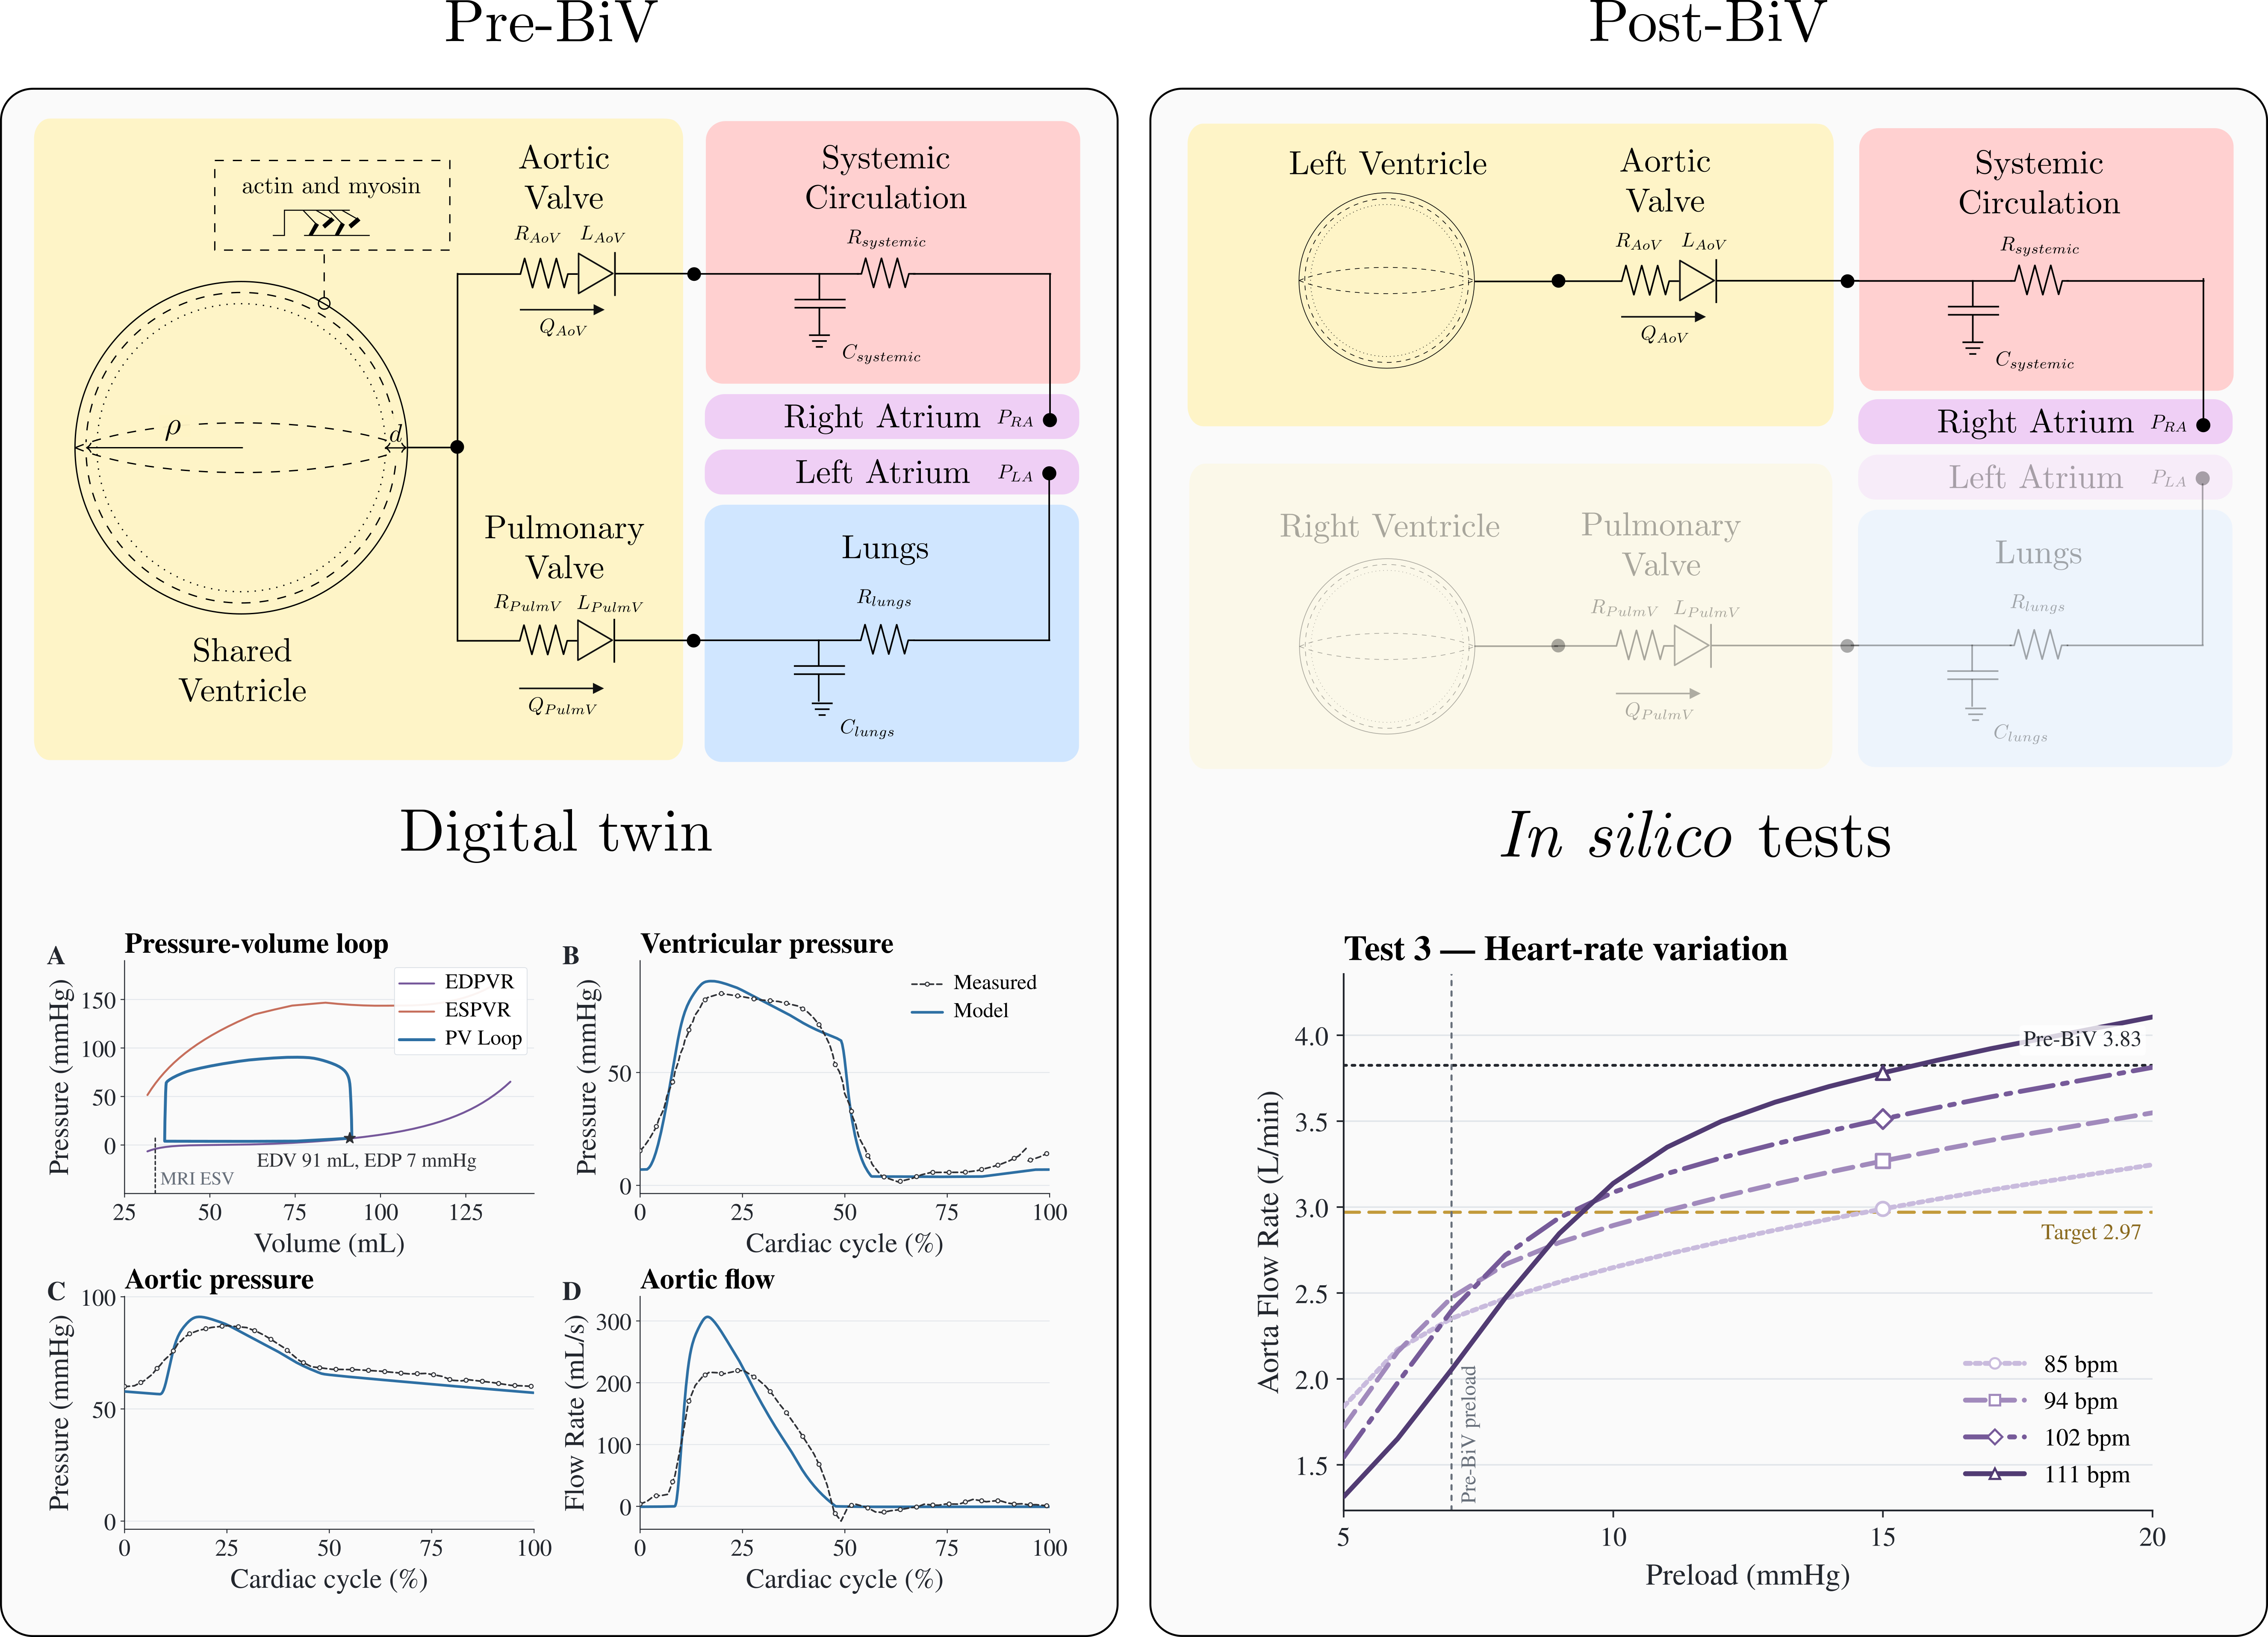
\includegraphics[width=1\columnwidth]{figures/schematics/DORV_BiV_model.png}
    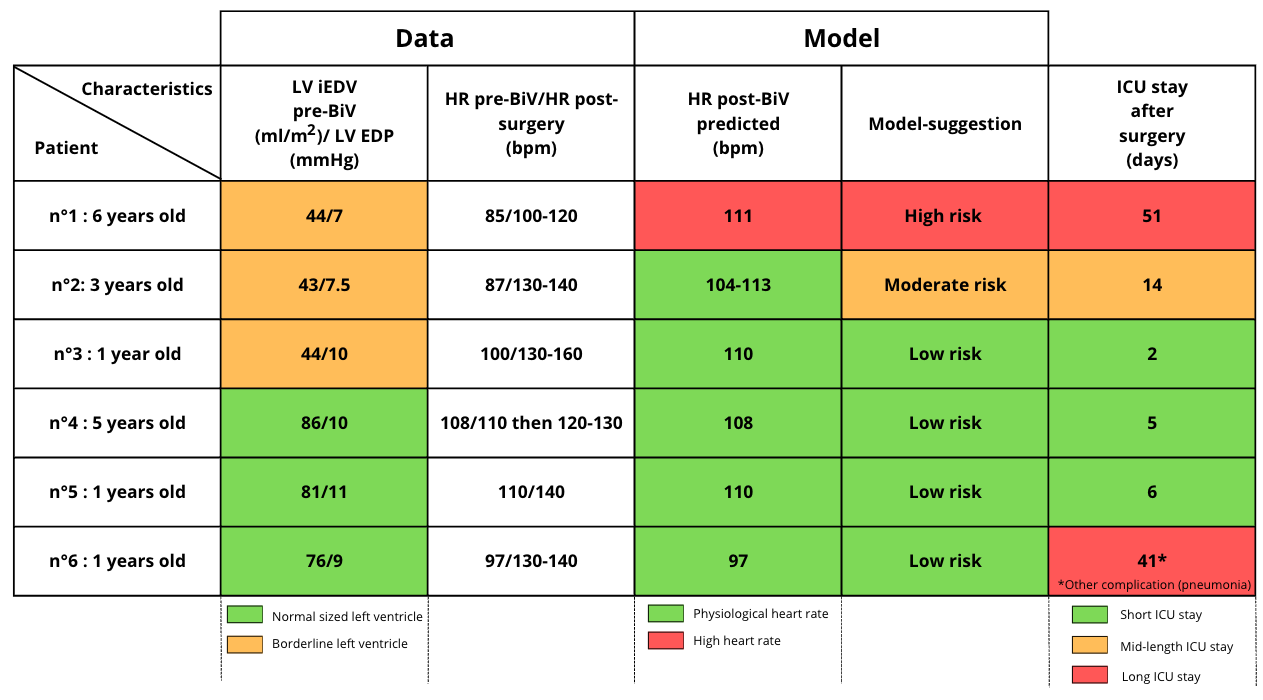
\includegraphics[width=0.75\columnwidth]{figures/simulations/DORV/DORV_table.png}           
    \caption{\textbf{Measurements prior to biventricular conversion, digital-twin risk prediction, and postoperative ICU length of stay in six patients undergoing the conversion. iEDV, end-diastolic volume indexed to body surface are; EDP, end-diastolic pressure; HR, heart rate; bpm, beat per minute. 
    }} 
    \label{fig:BiV_table}
    \vspace{-2pt}
\end{figure}


%\begin{figure}%[t!]
%    \centering
%    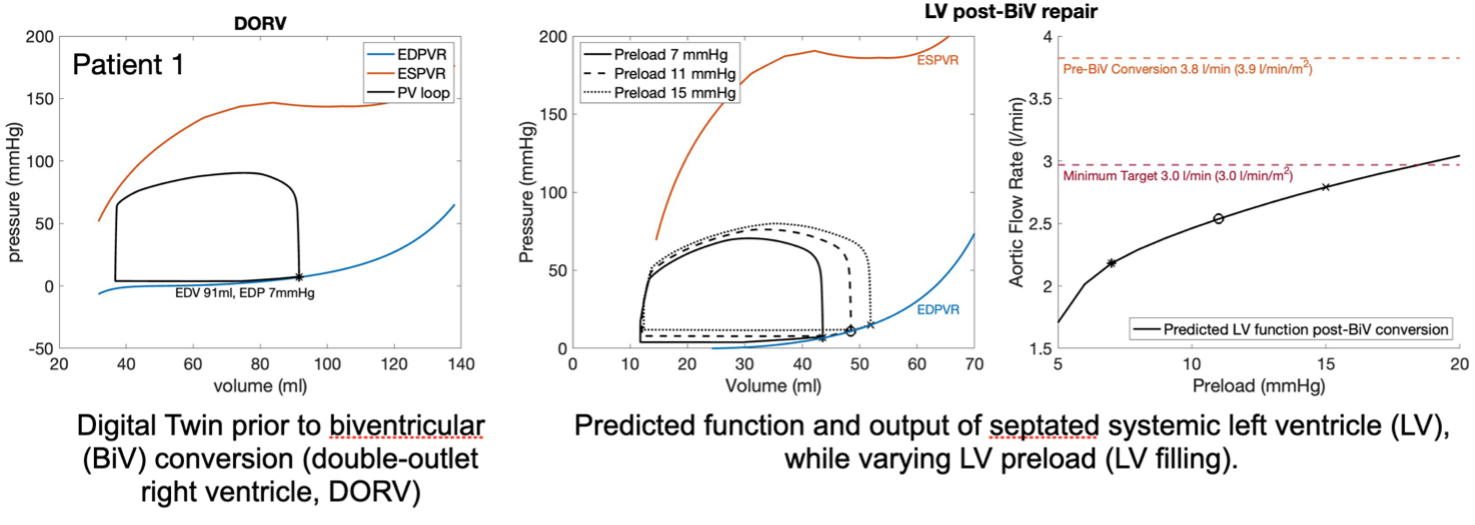
\includegraphics[width=1.0\columnwidth]{figures/simulations/DORV1a.png}
 %   \caption{\textbf{Model schematics for an example patient with double-outlet right ventricle and Glenn connection (superior vena cava to pulmonary ateries connection). 
  %  Digital Twin of Patient 1 in pilot\cite{chabiniok_Physiom2026abstract} prior to biventricular (BiV) conversion (double-outlet right ventricle, DORV, stage), created using patient's cardiac MRI and pressure catheter data. Middle and right panels: Predicted function of the left ventricle (LV) post BiV conversion, while varying the LV filling (preload). Note that the systemic left ventricle would reach the minimum target output at the rather high preload of above 15mmHg. EDPVR, end-diastolic pressure-volume relationship. ESPVR, end-systolic pressure-volume relationship
%    \textcolor{red}{WILL NOT BE INCLUDED}}} 
%    \label{fig:DORV1a}
%    \vspace{-2pt}
%\end{figure}

%\begin{figure}%[t!]
%    \centering
%    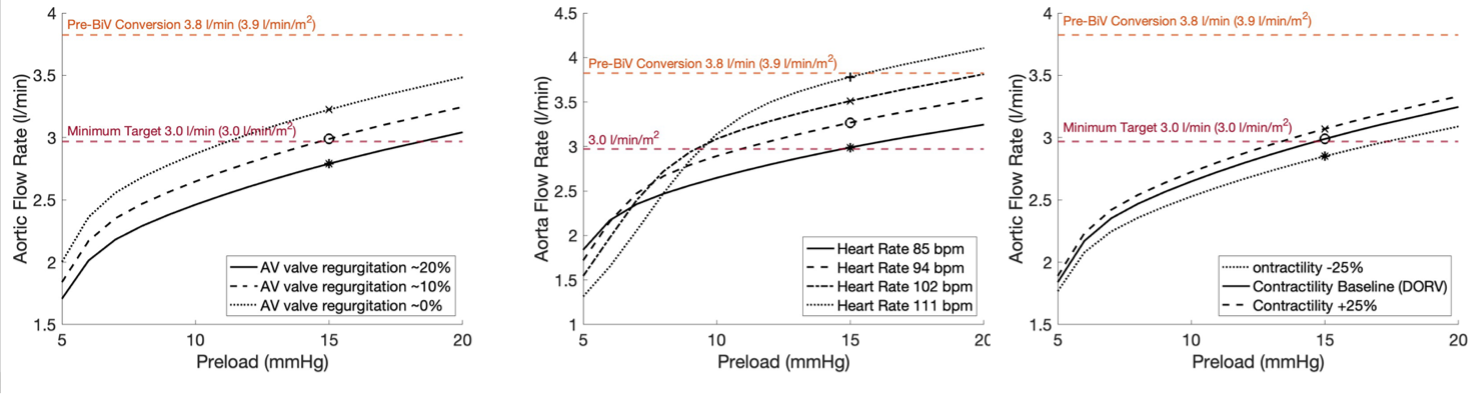
\includegraphics[width=1.0\columnwidth]{figures/simulations/DORV1b.png}
 %   \caption{\textbf{Predicted function of septated systemic LV in Patient 1 after in silico atrio-ventricular (AV) valve repair (original regurgitation fraction 20\%), with increasing the heart rate (from original value of 85 bpm), and inotropic support. The 30\% increase of HR to obtain sufficient systemic flow to a relatively high value for a 6-year old, at the borderline preload of 15 mmHg suggest that the BiV conversion may be successful, however, with a complicated post-surgery course. This was also reflected in the post-BiV surgery ICU stay of 51 days
 %   \textcolor{red}{WILL NOT BE INCLUDED}}} 
 %   \label{fig:DORV1b}
 %   \vspace{-2pt}
%\end{figure}

%\begin{figure}%[t!]
%    \centering
%    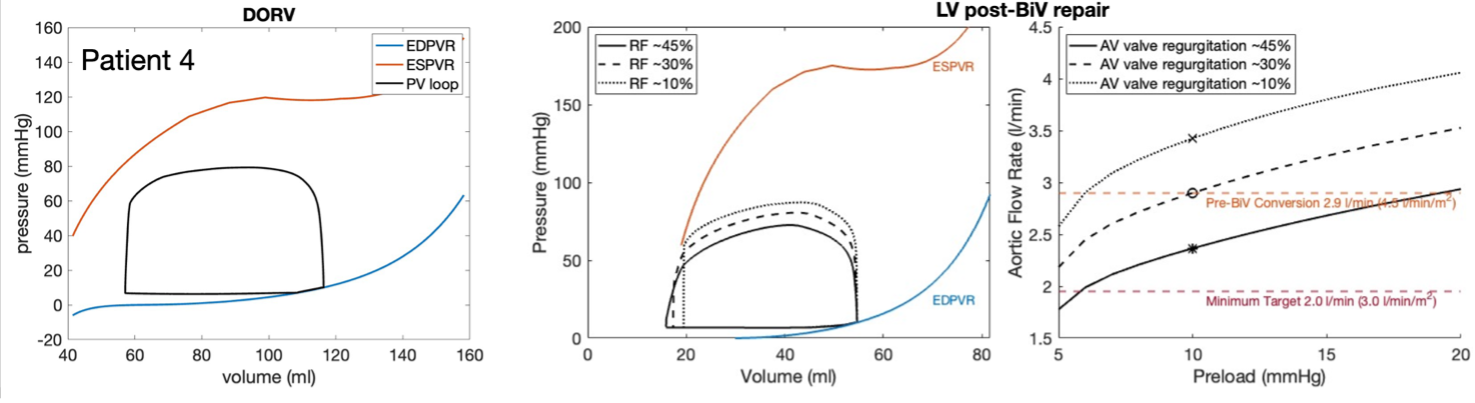
\includegraphics[width=1.0\columnwidth]{figures/simulations/DORV4.png}
%    \caption{\textbf{Left panel: Digital Twin of Patient 4 in pilot (Chabiniok et al., 2026) prior to biventricular (BiV) conversion (double-outlet right ventricle, DORV, stage. Middle and right panels: Predicted function of the left ventricle (LV) post BiV conversion, assuming different level of atrio-ventricular (AV) valve repair (regurgitation fraction 45\% as prior to repair and reduced to 10-30\%). The simulations suggest that reaching the pre-BiV conversion systemic flow will be relatively easy. This was also reflected in the shorter post-BiV surgery ICU (5 days).
%    \textcolor{red}{WILL NOT BE INCLUD}}} 
%    \label{fig:DORV4}
%    \vspace{-2pt}
%\end{figure}


%\begin{figure}%[t!]
%    \centering
%    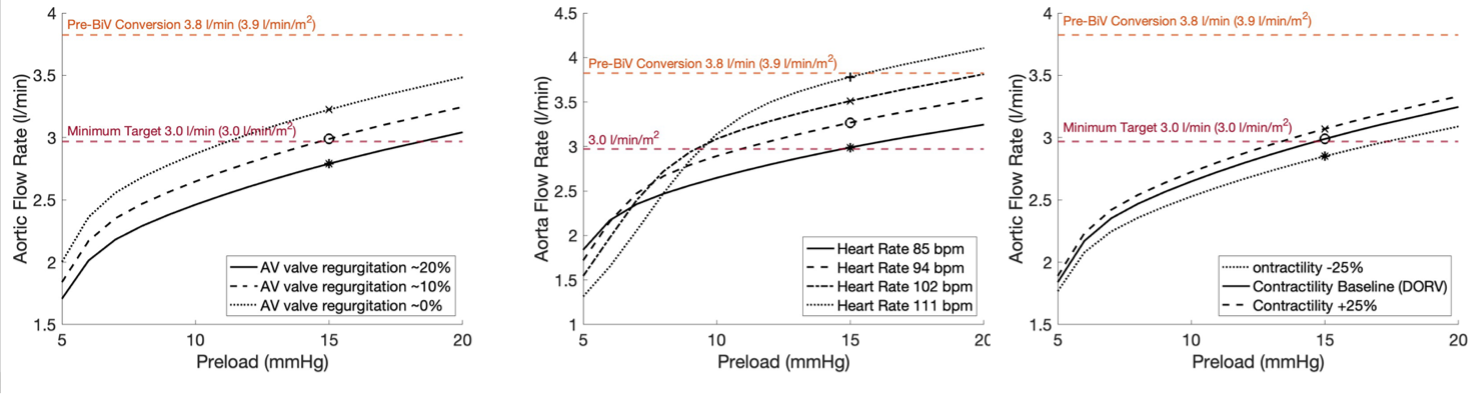
\includegraphics[width=1.0\columnwidth]{figures/simulations/DORV1b.png}
%    \caption{\textbf{Predicted function of septated systemic LV in Patient 1 after in silico atrio-ventricular (AV) valve repair (original regurgitation fraction 20\%), with increasing the heart rate (from original value of 85 bpm), and inotropic support. The 30\% increase of HR to obtain sufficient systemic flow to a relatively high value for a 6-year old, at the borderline preload of 15 mmHg suggest that the BiV conversion may be successful, however, with a complicated post-surgery course. This was also reflected in the post-BiV surgery ICU stay of 51 days
    %\textcolor{red}{WILL NOT BE INCLUDED}}} 
    %\label{fig:schematics}
%    \vspace{-2pt}
%\end{figure}

Hypothesis: The predicted non-favorable outcome (as defined above) will correlate with some indicators of the immediate clinical course during the post-surgery hospital stay (among which, we will use left atrial pressure in the first 48 hours; heart rate; inotrope requirement; end-organ dysfunction reflective of low cardiac output (BUN/Cr, LFTs, UOP); other hospital complications or re-interventions; ICU Length of Stay; Hospital Length of Stay).





\subsubsection{Aim 3: Predict ventricular growth after recruitment with a constrained mixture model}

\textbf{Rationale.} Ventricular recruitment deliberately overloads a borderline ventricle, by redirecting more inflow through its \gls*{av} valve and repairing a leaking \gls*{av} valve in a case-specific combination planned by the surgeon, to induce growth toward a size that can sustain a \gls*{biv} circulation. Whether a given ventricle will grow enough is currently unpredictable: it is judged only retrospectively at the post-recruitment \gls*{icmr} exam 8 to 15 months later, which is used to decide whether the heart can be septated (\gls*{biv} repair) or whether the child must instead proceed to single-ventricle palliation (Glenn, then Fontan). A ventricle that fails to grow has thus undergone recruitment surgery that, in the end, offered no benefit before the child enters the Fontan pathway anyway. \bfit{The clinically actionable target is therefore to predict, before recruitment, the risk of insufficient growth}, so that a child who would not benefit can be spared futile recruitment stages. Unlike the short-term re-adjustment predicted in Aim 2, this growth is a slow, load-driven adaptation of the myocardial tissue, mediated by the deposition and degradation of constituents in response to altered mechanical stimuli, that cannot be read from a pre-surgery snapshot. \bfit{Working hypothesis:} mechanically driven constituent turnover governs post-recruitment growth, so a constrained mixture model initialized from the pre-recruitment \gls*{dt} predicts insufficient growth more accurately than the size and pressure criteria used today.

\textbf{Feasibility and rigor of prior research.} The choice of model class is central to feasibility. Cardiac \gls*{gr} has most often been modeled with kinematic growth theory\cite{rodriguez94}, which prescribes the direction and extent of growth through an inelastic growth tensor. Such models have reproduced athlete's heart, ventricular dilation, and wall thickening\cite{goktepe10}, eccentric and concentric hypertrophy through sarcomerogenesis\cite{goktepe10}, heart failure\cite{costabal19,peirlinck19}, and acute myocardial infarction\cite{saez15}. They capture the shape and mass changes of \gls*{gr} efficiently, but they do not model why growth occurs: the extent and direction are prescribed rather than emerging from tissue turnover, growth is decoupled from cell-scale constituent production and removal, and the reversal of growth after a load is relieved is not captured\cite{gebauer23}. Predicting whether and when a borderline ventricle grows therefore requires a mechanistic model. The constrained mixture theory\cite{humphrey02a} tracks the production and removal of individual constituents within stressed configurations, so growth emerges from the mechanobiological processes observed in living tissue. Because its classical form must retain all past constituent configurations it is costly; the \gls*{hcmm}\cite{cyron16,braeu16} removes this cost by temporally homogenizing constituent deposition, making organ-scale \gls*{gr} tractable, with the growth of each constituent $i$ driven by the deviation of its fiber stress $\sigma^i$ from a homeostatic set-point $\sigma^i_h$ at a rate set by a gain parameter $k^i_\sigma$. Both capabilities this aim requires are already in hand and validated by our group: we developed and validated an \gls*{hcmm} of cardiac \gls*{gr} that predicts organ-scale ventricular change from constituent-level turnover and analyzed its mechanobiological stability and reversal, reproducing the reference constrained-mixture behavior at a fraction of the cost\cite{gebauer23}, and we made the formulation efficient for organ-scale simulation through adaptive integration of the history variables that otherwise dominate the cost\cite{gebauer24}. These build on the reduced-geometry heart model and PhysioBlocks implementation of Aims 1 and 2\cite{caruel13}, so the growth model shares the \gls*{dt} geometry, kinematics, and constitutive laws. Because Aim 3 operates on \glspl*{dt} constructed offline from stored \gls*{icmr} data, it is independent of the real-time pipeline of Aim 1. As an early go/no-go, in Year 1 we will reproduce a single retrospective paired case (pre- and post-recruitment \gls*{icmr}) end to end before scaling to the cohort.

\textbf{Sub-aim 3a: Formulate and calibrate a patient-specific constrained mixture model of the recruited ventricle (Years 1 to 3).} We will extend the spherical reduced-geometry ventricle of Aim 1 into an \gls*{hcmm} in which the myocardial wall is a mixture of a contractile myocyte constituent and a passive collagen and extracellular-matrix constituent, each with its own mass fraction, homeostatic stress, and turnover kinetics. Each patient's model will be initialized from the pre-recruitment \gls*{dt} (Aim 1), which synthesizes the \gls*{icmr} dataset: ventricular geometry (inner radius $R$ and wall thickness $d$ from cine-MRI end-diastolic and end-systolic volumes and myocardial mass), loading from the pressure-catheter waveforms (ventricular, atrial or wedge, and great-vessel pressures) and large-vessel flows (cardiac output and \gls*{av}-valve forward and reverse flow), and the homeostatic wall-stress set-point implied by the calibrated pre-recruitment equilibrium, imposed as the baseline about which growth is driven. Parameters that \gls*{icmr} constrains (geometry, loading, and baseline wall stress) will be patient-specific; constituent turnover rates, gain parameters $k^i_\sigma$, and mass fractions that cannot be measured in vivo will be set from our established cardiac priors\cite{gebauer23} and the constrained-mixture literature. The implementation will be verified against the published cardiac benchmark cases\cite{arostica25} and checked for mesh and step-size convergence before any patient application.

\textbf{Sub-aim 3b: Predict recruitment outcome and validate against the post-recruitment exam (Years 2 to 5).} For each recruited patient we will impose the post-recruitment mechanical loading, namely the increased inflow through the recruited chamber produced by the specific, surgeon-planned procedure (redirected \gls*{av}-valve inflow, \gls*{av}-valve repair), quantified from the measured change in \gls*{av}-valve inflow, and integrate the \gls*{hcmm} forward to the follow-up exam 8 to 15 months later. The intended redirection will be confirmed against the routine pre- and post-recruitment echocardiographic Doppler signals, which reliably capture the change in valvular inflow (echocardiographic volumes are not used). The model will predict the trajectory of end-diastolic and end-systolic volumes and myocardial mass, validated against the paired post-recruitment \gls*{icmr} exam in the recruitment subset (\textbf{expected N of roughly 10 to 15} over the award, drawn from the $\sim$50 complex \gls*{biv} cases per year, both borderline-left and borderline-right ventricles). Insufficient growth is defined a priori with the surgical team as failure to reach the \gls*{iedv} threshold used clinically to proceed to \gls*{biv} repair. Two endpoints are pre-specified: (1) agreement between predicted and measured \gls*{iedv} at follow-up, by Bland-Altman limits of agreement; and (2) accuracy in classifying insufficient growth, reported as sensitivity, specificity, and area under the ROC curve and compared head-to-head on the same patients against the current size and pressure criteria (DeLong test). The go/no-go for a subsequent multi-center study is a classification accuracy for insufficient growth that exceeds that of current criteria. Because the cohort is small, shared parameters (turnover, gains) will be evaluated by leave-one-out cross-validation to avoid optimistic bias. Sex and laterality will be recorded for every patient and examined as biological variables; borderline-left and borderline-right ventricles will be analyzed separately given their distinct loading.

\textbf{Expected results and interpretation.} We expect the model to reproduce the observed remodeling in ventricles that grew and, most importantly, to flag before surgery the ventricles that will not grow enough. A successful result (identification of insufficient growth that outperforms size and pressure criteria) would allow the team to spare those children futile recruitment stages, proceeding directly to single-ventricle palliation, while still recruiting ventricles predicted to benefit, thereby reducing the number of unnecessary complex surgeries on the path to definitive management. A partial result, in which the model captures the direction but not the magnitude of growth, would still stratify risk and localize the missing physiology (e.g., an unmodeled stimulus such as wall shear, or a growth-limiting factor), guiding refinement. A negative result (no predictive separation) would itself be informative, indicating that borderline-ventricle growth is governed by determinants not captured by mechanically driven turnover (e.g., intrinsic myocyte or genetic factors).

\textbf{Potential pitfalls and alternative strategies.} \textit{(i) Small sample size.} The recruitment subset is intrinsically small; we therefore frame Aim 3 as establishing predictive feasibility and an effect-size estimate to power a subsequent multi-center study, strengthening inference with leave-one-out validation rather than a held-out split. \textit{(ii) Non-identifiable parameters.} If population priors for turnover and gain do not generalize across this heterogeneous cohort, we will tighten the per-patient loading input using the measured change in \gls*{av}-valve inflow (great-vessel and valvular flow from \gls*{icmr}, corroborated by echocardiographic Doppler) and fit the single growth-gain parameter at the cohort level under leave-one-out, rather than relying on echocardiographic volumes, which are not sufficiently reliable in these patients. \textit{(iii) Geometry.} If the spherical reduction proves inadequate for the markedly non-ellipsoidal recruited chambers, we will map the \gls*{hcmm} onto the patient-specific 3D geometry validated in Aim 1, at higher computational cost but within the same constitutive framework. \textit{(iv) Stimulus form.} The driving stimulus for myocardial growth (fiber stress versus stretch, systolic versus diastolic) is not fully settled; we will compare stress- and stretch-driven formulations and report a sensitivity analysis over the gain parameters and homeostatic set-point. \textit{(v) Baseline homeostasis.} The assumption that the pre-recruitment state is at mechanobiological equilibrium may not hold in a chronically abnormal ventricle; we will bound this by perturbing the baseline set-point and reporting the spread in predicted growth.







\clearpage
\newpage

%%%%%%%%%%%%%%%%%%%%%%%%%%%%%%%%%%%%%%%%%%%%%%%%%%%%%%%%%%%%%%%%%%%%%%
%       EXAMPLES OF FIGURES 
%%%%%%%%%%%%%%%%%%%%%%%%%%%%%%%%%%%%%%%%%%%%%%%%%%%%%%%%%%%%%%%%%%%%%%

% ----- INSERT TOP FIGURE --------------------------------------------
%\begin{figure}[t!]
 %   \centering
 %   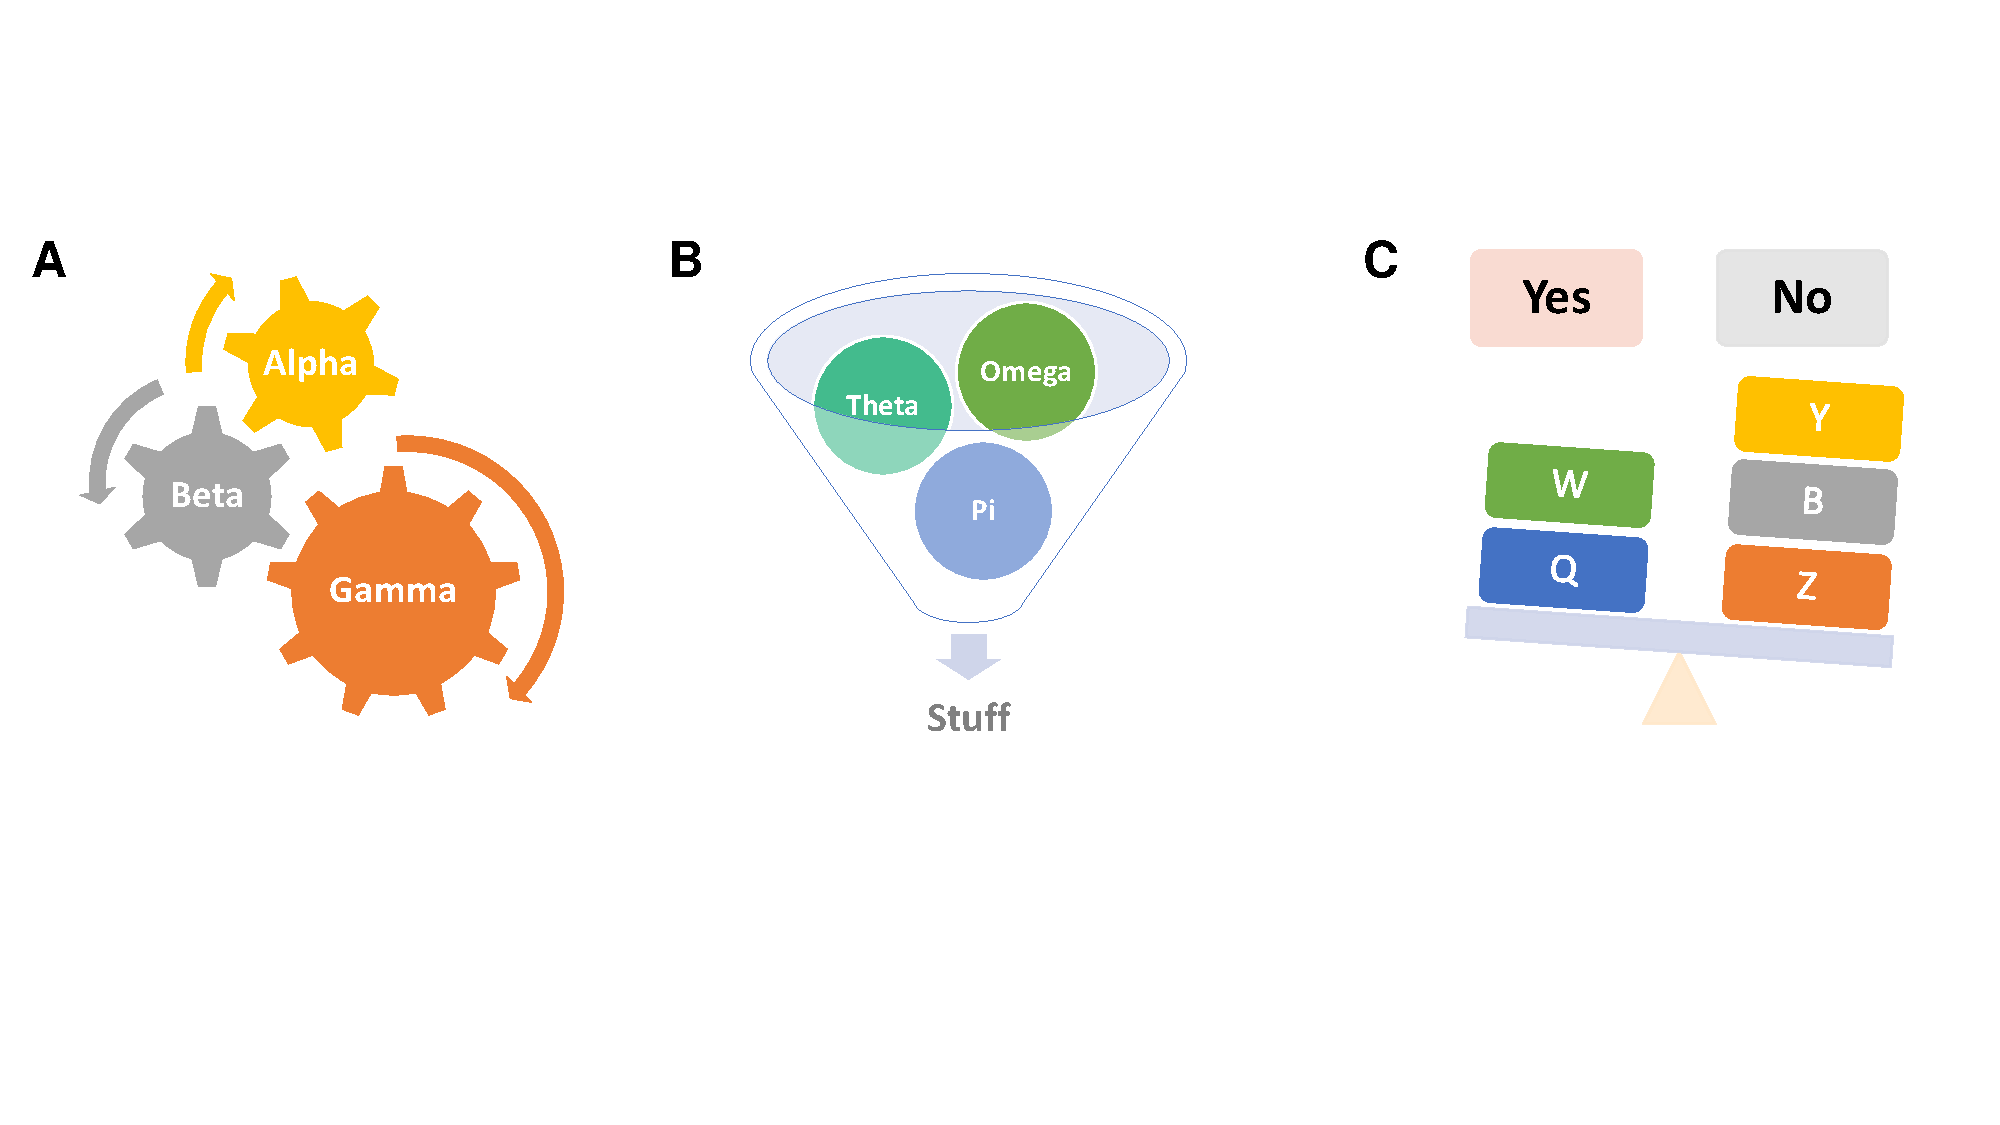
\includegraphics[width=1\columnwidth]{figures/figure_1.pdf}
 %   \caption{\textbf{Example of a top figure.} \lipsum[1][1-8]}
 %   \label{fig:figure_1}
 %   \vspace{-2pt}
%\end{figure}
% ----- END FIGURE ---------------------------------------------------

%\textbf{EXAMPLES OF TOP, WRAPPED AND BOTTOM FIGURES}

% ----- INSERT WRAP FIGURE -------------------------------------------
%\begin{wrapfigure}{r}{0.30\columnwidth}
%    \vspace{-15pt}
%    \centering
%    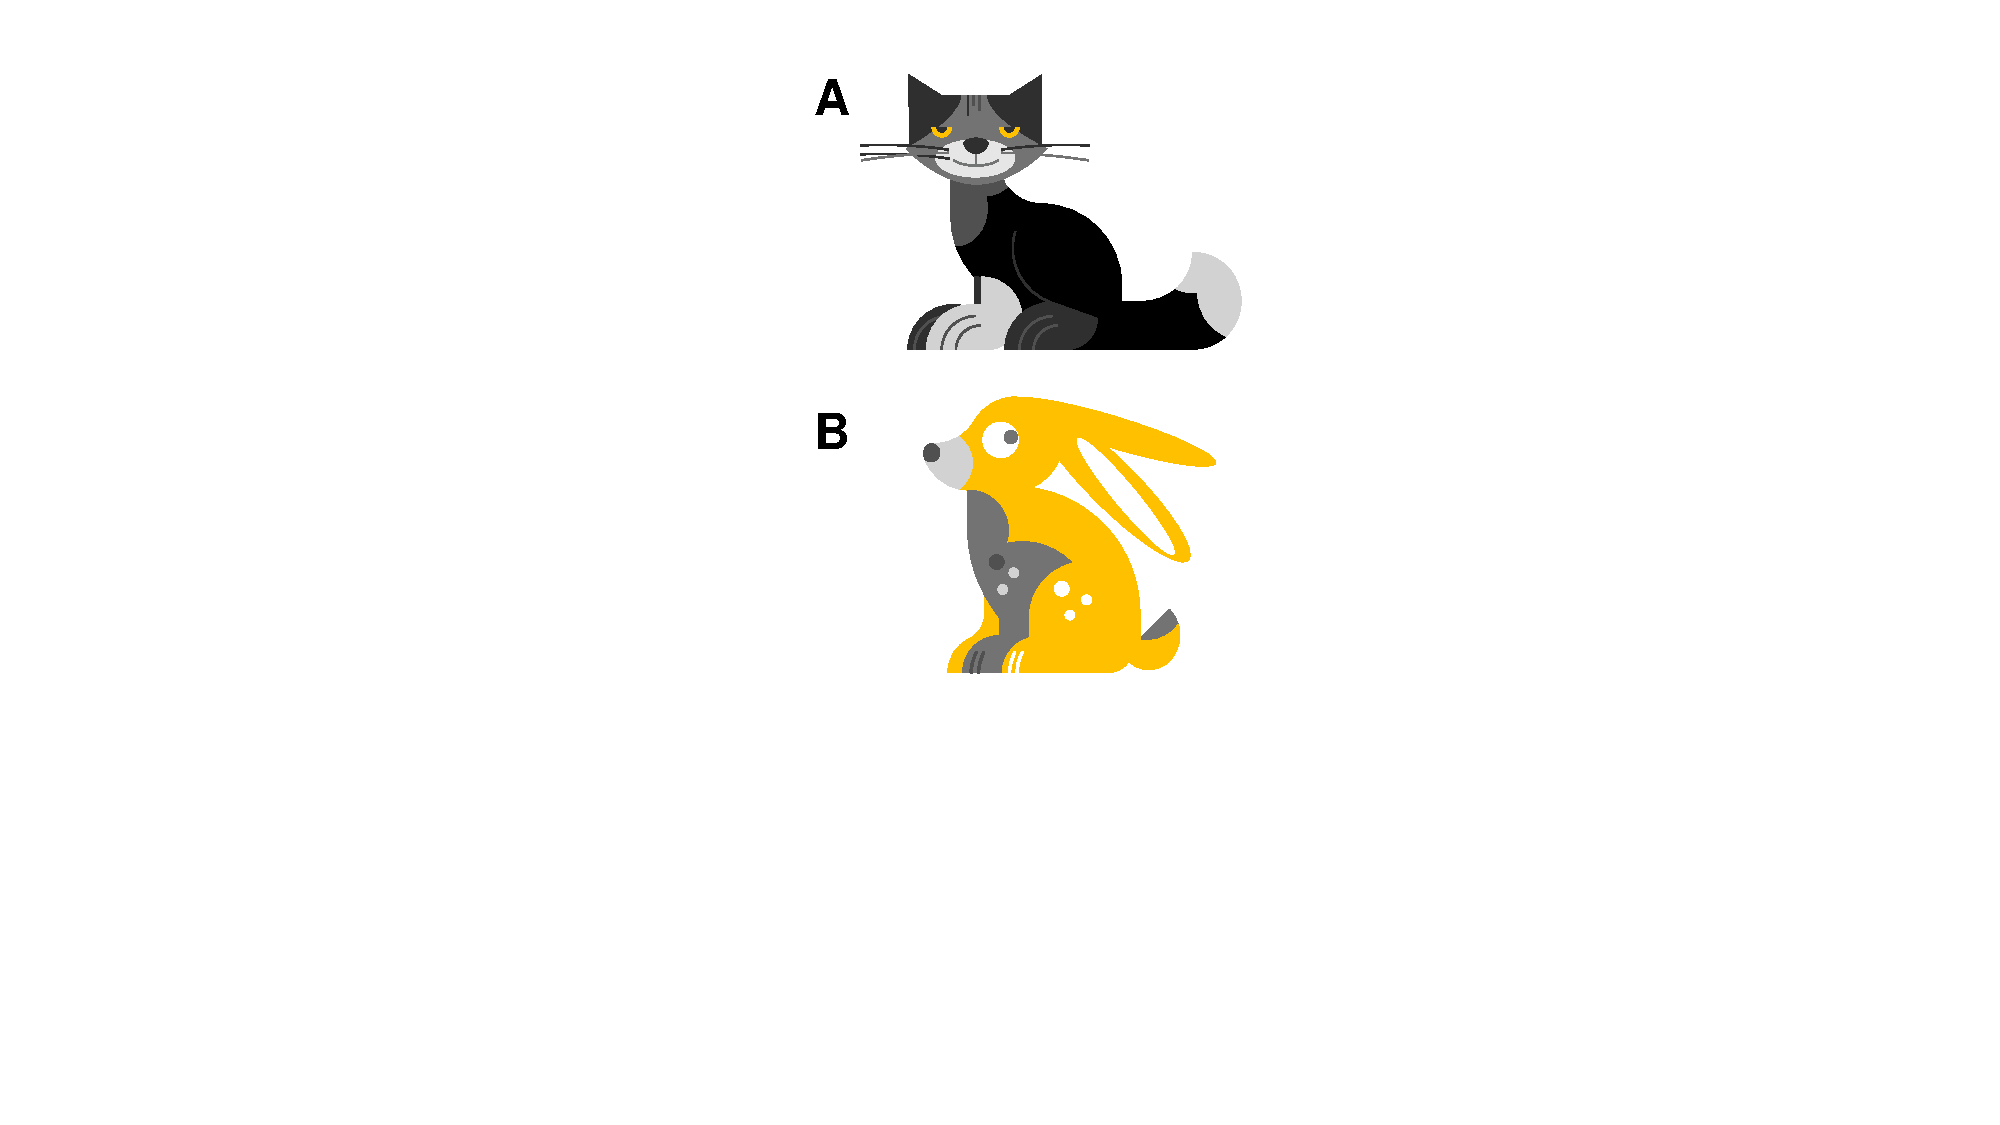
\includegraphics[width=0.30\columnwidth]{figures/figure_3.pdf} 
%    \caption{\textbf{Example of a wrapped figure.} \lipsum[1][1-4]}
%    \label{fig:figure_3}
%    \vspace{-15pt}
%\end{wrapfigure}
% ----- END FIGURE ---------------------------------------------------

%See Figures \ref{fig:figure_1}, \ref{fig:figure_2} and \ref{fig:figure_3}.

%\lipsum[4-6] 

% ----- INSERT BOTTOM FIGURE -----------------------------------------
%\begin{figure}[b!]
%    \centering
%    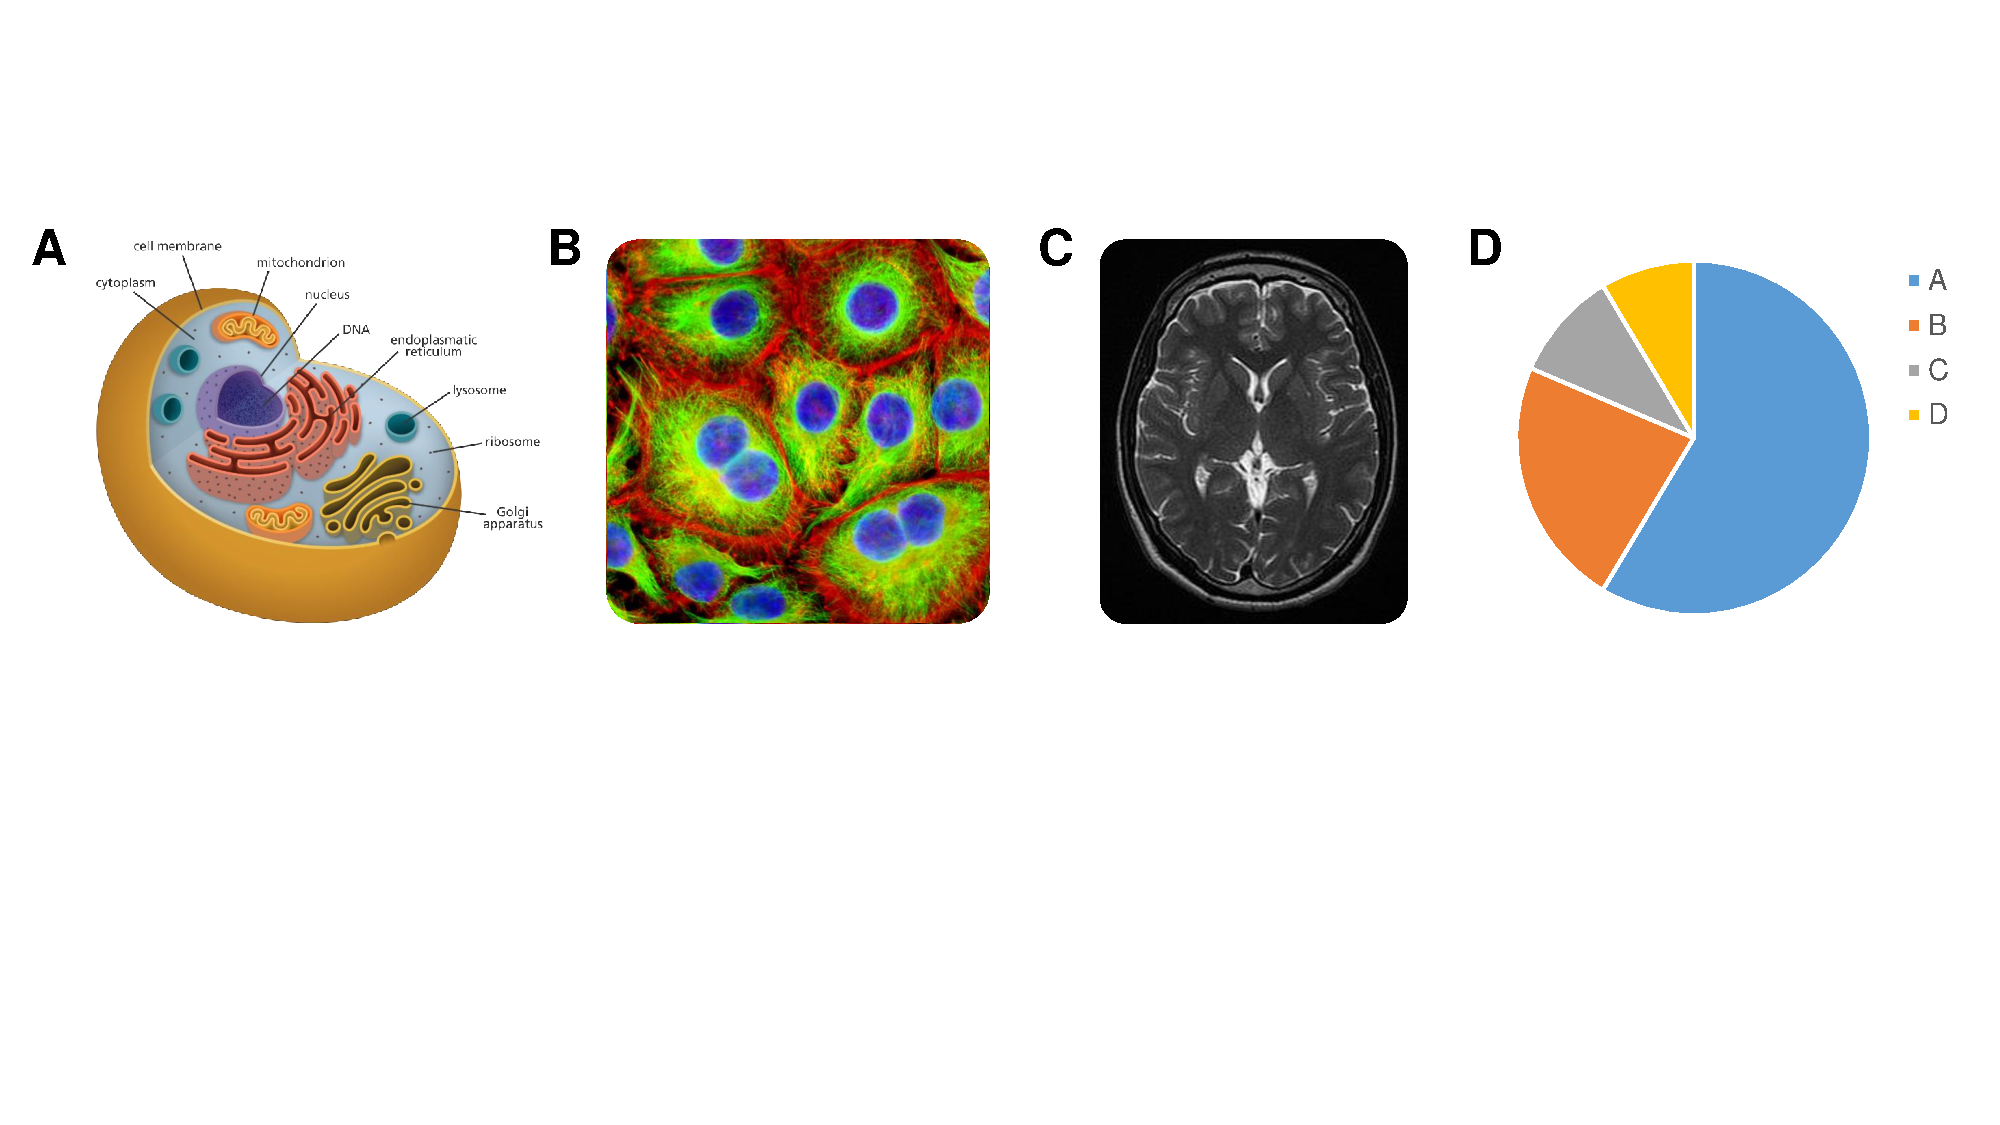
\includegraphics[width=1\linewidth]{figures/figure_2.pdf}
%    \caption{\textbf{Example of a bottom figure.} \lipsum[1][1-8]}
%    \label{fig:figure_2}
%    \vspace{-12pt}
%\end{figure}
% ----- END FIGURE ---------------------------------------------------

\clearpage

% %%%%%%%%%%%%%%%%%%%%%%%%%%%%%%%%%%%%%%%%%%%%%%%%%%%%%%%%%%%%%%%%%%%%%%
% %       EXAMPLES OF TABLES 
% %%%%%%%%%%%%%%%%%%%%%%%%%%%%%%%%%%%%%%%%%%%%%%%%%%%%%%%%%%%%%%%%%%%%%%

% % ----- INSERT TABLE -------------------------------------------------
% \begin{table}[t]
%     \centering
%     \caption{\textbf{Example of a top table.} \lipsum[32][1-7]}
%     \footnotesize
%     \begin{tabular}{>{\raggedright\arraybackslash}m{0.25\columnwidth} >{\centering\arraybackslash}m{0.25\columnwidth} >{\raggedleft\arraybackslash}m{0.15\columnwidth} >{\raggedleft\arraybackslash}m{0.14\columnwidth} >{\raggedleft\arraybackslash}m{0.10\columnwidth}}
%         \hline
%         \textbf{AAA} & \textbf{BBB} & \textbf{CCC} & \textbf{DDD} & \textbf{EEE} \\      
%         \hline
%         aaa & bbb & ccc & ddd & eee \\
%         \hline
%         \blah & 0 & 0 & 0 & 0 \\
%         \blah & 0 & 0 & 0 & 0 \\
%         \blah & 0 & 0 & 0 & 0 \\
%         \hline
%         \blah & 0 & 0 & 0 & 0 \\
%         \hline   
%         \end{tabular}
%     \label{tab:table_1}
% \end{table}
% % ----- END TABLE ----------------------------------------------------

% \textbf{EXAMPLES OF TOP AND WRAPPED TABLES}

% See Tables \ref{tab:table_1} and \ref{tab:table_2}.

% \lipsum[2]

% % ----- INSERT TABLE -------------------------------------------------
% \begin{wraptable}{r}{0.50\columnwidth}
%     \vspace{-12pt}
%     \caption{\textbf{Example of a wrapped table.} \lipsum[1][1-4]}
%     \vspace{-15pt}
%     \centering
%     \footnotesize
%     \begin{tabular}{>{\raggedright\arraybackslash}m{0.17\columnwidth} >{\centering\arraybackslash}m{0.16\columnwidth} >{\raggedleft\arraybackslash}m{0.10\columnwidth}} \\ 
%         \hline
%         \textbf{AAA} & \textbf{BBB} & \textbf{CCC} \\
%         \hline
%         aaa & bbb & ccc \\  
%         \hline
%         \blah & 0 & 0 \\  
%         \blah & 0 & 0 \\
%         \blah & 0 & 0 \\
%         \hline
%         \blah & 0 & 0 \\ 
%         \hline
%     \end{tabular}
%     \label{tab:table_2}
%     \vspace{-10pt}
% \end{wraptable} 
% % ----- END TABLE ----------------------------------------------------

% \lipsum[1] 

% \clearpage

% %%%%%%%%%%%%%%%%%%%%%%%%%%%%%%%%%%%%%%%%%%%%%%%%%%%%%%%%%%%%%%%%%%%%%%
% %       EXAMPLES OF ALGORITHMS 
% %%%%%%%%%%%%%%%%%%%%%%%%%%%%%%%%%%%%%%%%%%%%%%%%%%%%%%%%%%%%%%%%%%%%%%

% % ----- INSERT ALGORITHM ---------------------------------------------
% \begin{algorithm}[t!]
%     \caption{\textbf{Example of a top algorithm.} \lipsum[1][1-4]}
%     \footnotesize
%     \rule{1\columnwidth}{0.5pt}
%     \begin{algorithmic}
%         \Require $n \geq 0$
%         \Ensure $y = x^n$
%         \State $y \gets 1$
%         \State $X \gets x$
%         \State $N \gets n$
%         \While{$N \neq 0$}
%             \If{$N$ is even}
%                 \State $X \gets X \times X$
%                 \State $N \gets \frac{N}{2}$  \Comment{This is a comment}
%             \ElsIf{$N$ is odd}
%                 \State $y \gets y \times X$
%                 \State $N \gets N - 1$
%             \EndIf
%         \EndWhile
%     \end{algorithmic}
%     \vspace{-6pt}
%     \rule{1\columnwidth}{0.5pt}
%     \label{alg:algorithm_1}
%     \vspace{-10pt}
% \end{algorithm}
% % ----- END ALGORITHM ------------------------------------------------

% \textbf{EXAMPLES OF TOP AND WRAPPED ALGORITHMS}

% See Algorithms \ref{alg:algorithm_1} and \ref{alg:algorithm_2}.

% \lipsum[2]

% % ----- INSERT WRAP ALGORITHM ----------------------------------------
% \begin{wrapfigure}{r}{0.50\columnwidth}
%     \vspace{-18pt}
%     \centering
%     \begin{minipage}{0.50\columnwidth}
%         \begin{algorithm}[H]
%         \footnotesize
%         \rule{1\columnwidth}{0.5pt}
%         \caption{\textbf{Example of a wrapped algorithm.} \lipsum[1][1-4]}
%             \begin{algorithmic}[1]  % [1] = add line numbering
%                 \Require $n \geq 0$
%                 \Ensure $y = x^n$
%                 \State $y \gets 1$
%                 \State $X \gets x$
%                 \State $N \gets n$
%                 \While{$N \neq 0$}
%                     \If{$N$ is even}
%                         \State $X \gets X \times X$
%                         \State $N \gets \frac{N}{2}$ \Comment{This is a comment}
%                     \ElsIf{$N$ is odd}
%                         \State $y \gets y \times X$
%                         \State $N \gets N - 1$
%                     \EndIf
%                 \EndWhile
%             \end{algorithmic}
%             \vspace{-6pt}
%             \rule{1\columnwidth}{0.5pt}
%             \vspace{5pt}
%             \label{alg:algorithm_2}
%         \end{algorithm}
%     \end{minipage}
%     \vspace{-30pt}
% \end{wrapfigure}
% % ----- END ALGORITHM ------------------------------------------------

% \lipsum[3-4] 

% \clearpage

% %%%%%%%%%%%%%%%%%%%%%%%%%%%%%%%%%%%%%%%%%%%%%%%%%%%%%%%%%%%%%%%%%%%%%%
% %       PROTECTION OF HUMAN SUBJECTS
% %%%%%%%%%%%%%%%%%%%%%%%%%%%%%%%%%%%%%%%%%%%%%%%%%%%%%%%%%%%%%%%%%%%%%% 
% \section*{Protection of Human Subjects} 

% ~

% % ====================================================================
% %       RISKS TO HUMAN SUBJECTS
% % ====================================================================
% \subsection*{Risks to Human Subjects}

% % ===== HUMAN SUBJECTS INVOLVEMENT, CHARACTERISTICS, AND DESIGN ======
% \subsubsection*{Human Subjects Involvement, Characteristics, and Design}

% \lipsum[2]

% % ===== STUDY PROCEDURES, MATERIALS, AND POTENTIAL RISKS =============
% \subsubsection*{Study Procedures, Materials, and Potential Risks}

% \lipsum[2]

% ~

% % ====================================================================
% %       ADEQUACY OF PROTECTION AGAINST RISKS
% % ====================================================================
% \subsection*{Adequacy of Protection Against Risks}

% % ===== INFORMED CONSENT AND ASSENT ==================================
% \subsubsection*{Informed Consent and Assent}

% \lipsum[2]

% % ===== PROTECTIONS AGAINST RISK =====================================
% \subsubsection*{Protections Against Risk}

% \lipsum[2]

% \vspace{5pt}

% % ===== VULNERABLE SUBJECTS ==========================================
% \subsubsection*{Vulnerable Subjects}

% \lipsum[2]

% ~

% % ====================================================================
% %       POTENTIAL BENEFITS OF THE PROPOSED RESEARCH TO HUMAN SUBJECTS AND OTHERS
% % ====================================================================
% \subsection*{Potential Benefits of the Proposed Research to Human Subjects and Others}

% \lipsum[2]

% ~

% % ====================================================================
% %       IMPORTANCE OF THE KNOWLEDGE TO BE GAINED
% % ====================================================================
% \subsection*{Importance of the Knowledge to be Gained}

% \lipsum[2]

% \newpage

%%%%%%%%%%%%%%%%%%%%%%%%%%%%%%%%%%%%%%%%%%%%%%%%%%%%%%%%%%%%%%%%%%%%%%
%       REFERENCES
%%%%%%%%%%%%%%%%%%%%%%%%%%%%%%%%%%%%%%%%%%%%%%%%%%%%%%%%%%%%%%%%%%%%%% 
\clearpage
\section*{\normalsize{REFERENCES CITED \textnormal{(\textbf{PIs}, \underline{Collaborators})}}}
\bibliographystyle{mrp}
\bibliography{references,martin_highlighted}
\end{document}

%%%%%%%%%%%%%%%%%%%%%%%%%%%%%%%%%%%%%%%%%%%%%%%%%%%%%%%%%%%%%%%%%%%%%%
%       PROGRESS REPORT PUBLICATION LIST (For renewal only)
%%%%%%%%%%%%%%%%%%%%%%%%%%%%%%%%%%%%%%%%%%%%%%%%%%%%%%%%%%%%%%%%%%%%%% 
\section*{Progress Report Publication List}

\renewal

~

\begin{enumerate}
   
    \item Publication 1

    \item Publication 2

    \item Publication 3

\end{enumerate}

\newpage

%%%%%%%%%%%%%%%%%%%%%%%%%%%%%%%%%%%%%%%%%%%%%%%%%%%%%%%%%%%%%%%%%%%%%%
%       DATA AND SAFETY MONITORING PLAN (DSMP)
%%%%%%%%%%%%%%%%%%%%%%%%%%%%%%%%%%%%%%%%%%%%%%%%%%%%%%%%%%%%%%%%%%%%%% 
\section*{Data and Safety Monitoring Plan (DSMP)}

~

\lipsum[2]

\newpage

%%%%%%%%%%%%%%%%%%%%%%%%%%%%%%%%%%%%%%%%%%%%%%%%%%%%%%%%%%%%%%%%%%%%%%
%       DATA MANAGEMENT AND SHARING (DMS) PLAN
%%%%%%%%%%%%%%%%%%%%%%%%%%%%%%%%%%%%%%%%%%%%%%%%%%%%%%%%%%%%%%%%%%%%%% 
\section*{Data Management and Sharing (DMS) Plan}

~ 

% ====================================================================
%       ELEMENT 1: DATA TYPE
% ====================================================================
\subsection*{Element 1: Data Type}

% ===== A. TYPES AND AMOUNT OF SCIENTIFIC DATA EXPECTED TO BE GENERATED IN THE PROJECT
\subsubsection*{A. Types and amount of scientific data expected to be generated in the project:} 

Summarize the types and estimated amount of scientific data expected to be generated in the project.

% ===== B. SCIENTIFIC DATA THAT WILL BE PRESERVED AND SHARED, AND THE RATIONALE FOR DOING SO
\subsubsection*{B. Scientific data that will be preserved and shared, and the rationale for doing so:}

Describe which scientific data will be preserved and shared and provide the rationale for this decision. 

% ===== C. METADATA, OTHER RELEVANT DATA, AND ASSOCIATED DOCUMENTATION
\subsubsection*{C. Metadata, other relevant data, and associated documentation: }

Briefly list the metadata, other relevant data, and any associated documentation (e.g., study protocols and data collection instruments) that will be made accessible to facilitate interpretation of the scientific data.

~

% ====================================================================
%       ELEMENT 2: RELATED TOOLS, SOFTWARE AND/OR CODE
% ====================================================================
\subsection*{Element 2: Related Tools, Software and/or Code}

State whether specialized tools, software, and/or code are needed to access or manipulate shared scientific data, and if so, provide the name(s) of the needed tool(s) and software and specify how they can be accessed.

~

% ====================================================================
%       ELEMENT 3: STANDARDS
% ====================================================================
\subsection*{Element 3: Standards}

State what common data standards will be applied to the scientific data and associated metadata to enable interoperability of datasets and resources, and provide the name(s) of the data standards that will be applied and describe how these data standards will be applied to the scientific data generated by the research proposed in this project. If applicable, indicate that no consensus standards exist.

~

% ====================================================================
%       ELEMENT 4: DATA PRESERVATION, ACCESS, AND ASSOCIATED TIMELINES
% ====================================================================
\subsection*{Element 4: Data Preservation, Access, and Associated Timelines}

% ===== A. Repository where scientific data and metadata will be archived
\subsubsection*{A. Repository where scientific data and metadata will be archived:} 

Provide the name of the repository(ies) where scientific data and metadata arising from the project will be archived; see Selecting a Data Repository).

% ===== B. HOW SCIENTIFIC DATA WILL BE FINDABLE AND IDENTIFIABLE ===== 
\subsubsection*{B. How scientific data will be findable and identifiable: }

Describe how the scientific data will be findable and identifiable, i.e., via a persistent unique identifier or other standard indexing tools.

% ===== C. WHEN AND HOW LONG THE SCIENTIFIC DATA WILL BE MADE AVAILABLE
\textbf{C. When and how long the scientific data will be made available: }
 
Describe when the scientific data will be made available to other users (i.e., no later than time of an associated publication or end of the performance period, whichever comes first) and for how long data will be available.

~

% ====================================================================
%       ELEMENT 5: ACCESS, DISTRIBUTION, OR REUSE CONSIDERATIONS
% ====================================================================
\subsection*{Element 5: Access, Distribution, or Reuse Considerations}

% ===== A. FACTORS AFFECTING SUBSEQUENT ACCESS, DISTRIBUTION, OR REUSE OF SCIENTIFIC DATA
\subsubsection*{A. Factors affecting subsequent access, distribution, or reuse of scientific data:}

NIH expects that in drafting Plans, researchers maximize the appropriate sharing of scientific data. Describe and justify any applicable factors or data use limitations affecting subsequent access, distribution, or reuse of scientific data related to informed consent, privacy and confidentiality protections, and any other considerations that may limit the extent of data sharing. 

% ===== B. WHETHER ACCESS TO SCIENTIFIC DATA WILL BE CONTROLLED ======
\subsubsection*{B. Whether access to scientific data will be controlled:}

State whether access to the scientific data will be controlled (i.e., made available by a data repository only after approval).

% ===== C. PROTECTIONS FOR PRIVACY, RIGHTS, AND CONFIDENTIALITY OF HUMAN RESEARCH PARTICIPANTS
\subsubsection*{C. Protections for privacy, rights, and confidentiality of human research participants:}

If generating scientific data derived from humans, describe how the privacy, rights, and confidentiality of human research participants will be protected (e.g., through de-identification, Certificates of Confidentiality, and other protective measures). 

~

% ====================================================================
%       ELEMENT 6: OVERSIGHT OF DATA MANAGEMENT AND SHARING
% ====================================================================
\subsection*{Element 6: Oversight of Data Management and Sharing}

Describe how compliance with this Plan will be monitored and managed, frequency of oversight, and by whom at your institution (e.g., titles, roles).

\newpage

%%%%%%%%%%%%%%%%%%%%%%%%%%%%%%%%%%%%%%%%%%%%%%%%%%%%%%%%%%%%%%%%%%%%%%
%       TARGETED/PLANNED ENROLLMENT TABLE
%%%%%%%%%%%%%%%%%%%%%%%%%%%%%%%%%%%%%%%%%%%%%%%%%%%%%%%%%%%%%%%%%%%%%% 
\section*{Targeted/Planned Enrollment Table}

~

\begin{lyxlist}{000.000.000.000.000.000.000.000.000.000.000}
    \item [\textbf{Study~Title:}] Study title
    \item [\textbf{Delayed~Onset~Study?}] Yes/No
    \item [\textbf{Enrollment~Type:}] Planned/Cumulative
    \item [\textbf{Using~an~Existing~Dataset~or~Resource:}] Yes/No
    \item [\textbf{Enrollment~Location:}] Domestic/Foreign
    \item [\textbf{Clinical~Trial:}] Yes/No
    \item [\textbf{NIH-Defined~Phase~III~Clinical~Trial:}] Yes/No
    \item [\textbf{Comments:}] \blah
\end{lyxlist}

~

~

% ----- INSERT TABLE -------------------------------------------------
\begin{table}[h]
    \centering
    \small
        \begin{tabular}{|>{\centering}m{50mm}|>{\centering}m{20mm}|>{\centering}m{20mm}|>{\centering}m{20mm}|>{\centering}m{20mm}|>{\centering}m{20mm}|}
        \hline 
        ~ & \multicolumn{4}{c|}{\textbf{Ethnic Categories}} & \tabularnewline
        \cline{2-5} 
        \textbf{Racial categories} & \multicolumn{2}{c|}{\textbf{Not Hispanic or Latino}} & \multicolumn{2}{c|}{\textbf{Hispanic or Latino}} & \textbf{Total} \tabularnewline
        \cline{2-5} & \textbf{Female} & \textbf{Male} & \textbf{Female} & \textbf{Male} & \tabularnewline
        \hline 
        American Indian/Alaska Native & 0 & 0 & 0 & 0 & \textbf{0} \tabularnewline
        \hline 
        Asian & 0 & 0 & 0 & 0 & \textbf{0} \tabularnewline
        \hline 
        Native Hawaiian or Other Pacific Islander & 0 & 0 & 0 & 0 & \textbf{0} \tabularnewline
        \hline 
        Black or African American & 0 & 0 & 0 & 0 & \textbf{0} \tabularnewline
        \hline 
        White & 0 & 0 & 0 & 0 & \textbf{0} \tabularnewline
        \hline 
        More than One Race & 0 & 0 & 0 & 0 & \textbf{0} \tabularnewline
        \hline 
        Total & \textbf{0} & \textbf{0} & \textbf{0} & \textbf{0} & \textbf{0} \tabularnewline
        \hline
    \end{tabular}
\end{table}
% ----- END TABLE ----------------------------------------------------

\newpage

%%%%%%%%%%%%%%%%%%%%%%%%%%%%%%%%%%%%%%%%%%%%%%%%%%%%%%%%%%%%%%%%%%%%%%
%       INCLUSION OF WOMEN AND MINORITIES
%%%%%%%%%%%%%%%%%%%%%%%%%%%%%%%%%%%%%%%%%%%%%%%%%%%%%%%%%%%%%%%%%%%%%% 
\section*{Inclusion of Women and Minorities}

~

\lipsum[6]

\newpage

%%%%%%%%%%%%%%%%%%%%%%%%%%%%%%%%%%%%%%%%%%%%%%%%%%%%%%%%%%%%%%%%%%%%%%
%       INCLUSION OF INDIVIDUALS ACROSS THE LIFESPAN
%%%%%%%%%%%%%%%%%%%%%%%%%%%%%%%%%%%%%%%%%%%%%%%%%%%%%%%%%%%%%%%%%%%%%% 
\section*{Inclusion of Individuals Across the Lifespan}

~

\lipsum[11] 

\newpage

%%%%%%%%%%%%%%%%%%%%%%%%%%%%%%%%%%%%%%%%%%%%%%%%%%%%%%%%%%%%%%%%%%%%%%
%       RECRUITMENT AND RETENTION PLAN
%%%%%%%%%%%%%%%%%%%%%%%%%%%%%%%%%%%%%%%%%%%%%%%%%%%%%%%%%%%%%%%%%%%%%%
\section*{Recruitment and Retention Plan}

~

% ====================================================================
%       RECRUITMENT PLAN
% ====================================================================
\subsection*{Recruitment Plan}

\lipsum[12]

~

% ====================================================================
%       RETENTION PLAN
% ====================================================================
\subsection*{Retention Plan}

\lipsum[12]

\newpage

%%%%%%%%%%%%%%%%%%%%%%%%%%%%%%%%%%%%%%%%%%%%%%%%%%%%%%%%%%%%%%%%%%%%%%
%       STUDY TIMELINE
%%%%%%%%%%%%%%%%%%%%%%%%%%%%%%%%%%%%%%%%%%%%%%%%%%%%%%%%%%%%%%%%%%%%%%
\section*{Study Timeline}

~

% ----- INSERT TABLE -------------------------------------------------
\begin{table}[ht]
    \footnotesize
    \centering
    \begin{tabular}{m{8mm} m{17mm} m{60mm} m{5mm} m{5mm} m{5mm} m{5mm} m{5mm} m{5mm} m{5mm} m{5mm} m{5mm} m{5mm}}
        %
        \hline
        \textbf{Aims} & \textbf{Sub-Aims} & \textbf{Purpose} & \multicolumn{2}{c}{\textbf{Year 1}} & \multicolumn{2}{c}{\textbf{Year 2}} & \multicolumn{2}{c}{\textbf{Year 3}} & \multicolumn{2}{c}{\textbf{Year 4}} & \multicolumn{2}{c}{\textbf{Year 5}} \\
        \hline
        %
        \multirow{2}{8mm}{\textbf{1}} & \textbf{1.a} & Sub-aim 1.a & ~ & \cellcolor{darkgray} & \cellcolor{darkgray} & \cellcolor{darkgray} & \cellcolor{darkgray} & \cellcolor{darkgray} & \cellcolor{darkgray} & ~ & ~ & ~ \\
        %
        ~ & \textbf{1.b} & Sub-aim 1.b & \cellcolor{darkgray} & \cellcolor{darkgray} & \cellcolor{darkgray} & \cellcolor{darkgray} & \cellcolor{darkgray} & \cellcolor{darkgray} & ~ & ~ & ~ & ~ \\
        \hline 
        \multirow{2}{8mm}{\textbf{2}} & \textbf{2.a} & Sub-aim 2.a & \cellcolor{darkgray} & \cellcolor{darkgray} & \cellcolor{darkgray} & \cellcolor{darkgray} & \cellcolor{darkgray} & \cellcolor{darkgray} & ~ & ~ & ~ & ~ \\
        %
        ~ & \textbf{2.b} & Sub-aim 2.b & ~ & \cellcolor{darkgray} & \cellcolor{darkgray} & \cellcolor{darkgray} & \cellcolor{darkgray} & \cellcolor{darkgray} & \cellcolor{darkgray} & \cellcolor{darkgray} & \cellcolor{darkgray} & ~ \\
        \hline  
        \multirow{2}{8mm}{\textbf{3}} & \textbf{3.a} & Sub-aim 3.a & \cellcolor{darkgray} & \cellcolor{darkgray} & \cellcolor{darkgray} & \cellcolor{darkgray} & \cellcolor{darkgray} & \cellcolor{darkgray} & ~ & ~ & ~ & ~ \\
        %
        ~ & \textbf{3.b} & Sub-aim 3.b & ~ & ~ & ~ & ~ & \cellcolor{darkgray} & \cellcolor{darkgray} & \cellcolor{darkgray} & \cellcolor{darkgray} &\cellcolor{darkgray} & \cellcolor{darkgray} \\
        \hline        
    \end{tabular}
    \label{tab:timeline}
\end{table}
% ----- END TABLE ----------------------------------------------------

\newpage

%%%%%%%%%%%%%%%%%%%%%%%%%%%%%%%%%%%%%%%%%%%%%%%%%%%%%%%%%%%%%%%%%%%%%%
%       PROJECT SUMMARY
%%%%%%%%%%%%%%%%%%%%%%%%%%%%%%%%%%%%%%%%%%%%%%%%%%%%%%%%%%%%%%%%%%%%%%
\section*{Project Summary}

~

\lipsum[1]

\newpage

%%%%%%%%%%%%%%%%%%%%%%%%%%%%%%%%%%%%%%%%%%%%%%%%%%%%%%%%%%%%%%%%%%%%%%
%       PROJECT NARRATIVE
%%%%%%%%%%%%%%%%%%%%%%%%%%%%%%%%%%%%%%%%%%%%%%%%%%%%%%%%%%%%%%%%%%%%%%
\section*{Project Narrative}

~ 

\lipsum[2][1-3]

\newpage

%%%%%%%%%%%%%%%%%%%%%%%%%%%%%%%%%%%%%%%%%%%%%%%%%%%%%%%%%%%%%%%%%%%%%%
%       FACILITIES AND OTHER RESOURCES
%%%%%%%%%%%%%%%%%%%%%%%%%%%%%%%%%%%%%%%%%%%%%%%%%%%%%%%%%%%%%%%%%%%%%%
\section*{Facilities and Other Resources}

~

% ====================================================================
%      UNIVERSITY
% ====================================================================
\subsection*{ABC University}

\lipsum[8]

~

% ====================================================================
%       DEPARTMENT
% ====================================================================
\subsection*{Department of Stuff}

\lipsum[8]

~

% ====================================================================
%       RESEARCH CENTER
% ====================================================================
\subsection*{Research Center X}

\lipsum[8]

~

% ====================================================================
%       LABORATORY
% ====================================================================
\subsection*{Laboratory Y}

\lipsum[8]

~

\newpage

%%%%%%%%%%%%%%%%%%%%%%%%%%%%%%%%%%%%%%%%%%%%%%%%%%%%%%%%%%%%%%%%%%%%%%
%       MAJOR EQUIPMENT
%%%%%%%%%%%%%%%%%%%%%%%%%%%%%%%%%%%%%%%%%%%%%%%%%%%%%%%%%%%%%%%%%%%%%%
\section*{Major Equipment}

~

% ====================================================================
%       EQUIPMENT A
% ====================================================================
\subsection*{Equipment A}

\lipsum[55]

~

% ====================================================================
%       EQUIPMENT B
% ====================================================================
\subsection*{Equipment B}

\lipsum[55]

\newpage

%%%%%%%%%%%%%%%%%%%%%%%%%%%%%%%%%%%%%%%%%%%%%%%%%%%%%%%%%%%%%%%%%%%%%%
%       RESOURCE SHARING PLAN
%%%%%%%%%%%%%%%%%%%%%%%%%%%%%%%%%%%%%%%%%%%%%%%%%%%%%%%%%%%%%%%%%%%%%%
\section*{Resource Sharing Plan}

~

% ====================================================================
%       RESEARCH TOOLS
% ====================================================================
\subsection*{Research Tools}

\lipsum[2]

~

% ====================================================================
%      SHARING MODEL ORGANISMS
% ====================================================================
\subsection*{Sharing Model Organisms}

\lipsum[2]

\newpage

%%%%%%%%%%%%%%%%%%%%%%%%%%%%%%%%%%%%%%%%%%%%%%%%%%%%%%%%%%%%%%%%%%%%%%
%       MULTIPLE PD/PI LEADERSHIP PLAN
%%%%%%%%%%%%%%%%%%%%%%%%%%%%%%%%%%%%%%%%%%%%%%%%%%%%%%%%%%%%%%%%%%%%%%
\section*{Multiple PD/PI Leadership Plan}

~

% ====================================================================
%       PD/PI'S
% ====================================================================
\subsection*{PD/PI's }

\lipsum[66]

~

% ====================================================================
%      TIME COMMITMENT
% ====================================================================
\subsection*{Time Commitment}

\lipsum[66]

~

% ====================================================================
%       COLLABORATIVE EFFORT
% ====================================================================
\subsection*{Collaborative Effort}

\lipsum[66]

~

% ====================================================================
%       CONFLICT RESOLUTION
% ====================================================================
\subsection*{Conflict Resolution}

\lipsum[66]

~

% ====================================================================
%       COMMUNICATION PLAN 
% ====================================================================
\subsection*{Communication Plan}

\lipsum[66]

~

% ====================================================================
%       PROCESS FOR MAKING DECISIONS ON SCIENTIFIC DIRECTION
% ====================================================================
\subsection*{Process for Making Decisions on Scientific Direction}

\lipsum[66]

~

% ====================================================================
%       CONTACT PI
% ====================================================================
\subsection*{Contact PI}

\lipsum[66]

~

% ====================================================================
%       CHANGE IN PI LOCATION
% ====================================================================
\subsection*{Change in PI Location}

\lipsum[66]

\newpage

%%%%%%%%%%%%%%%%%%%%%%%%%%%%%%%%%%%%%%%%%%%%%%%%%%%%%%%%%%%%%%%%%%%%%%
%       AUTHENTICATION OF KEY BIOLOGICAL AND/OR CHEMICAL RESOURCES
%%%%%%%%%%%%%%%%%%%%%%%%%%%%%%%%%%%%%%%%%%%%%%%%%%%%%%%%%%%%%%%%%%%%%%
\section*{Authentication of Key Biological and/or Chemical Resources}

~

% ====================================================================
%       BIOLOGICAL RESOURCES
% ====================================================================
\subsection*{Biological Resources}

\lipsum[2]

~

% ====================================================================
%       CHEMICAL RESOURCES
% ====================================================================
\subsection*{Chemical Resources}

\lipsum[2]

\newpage

%%%%%%%%%%%%%%%%%%%%%%%%%%%%%%%%%%%%%%%%%%%%%%%%%%%%%%%%%%%%%%%%%%%%%%
%       BUDGET JUSTIFICATION
%%%%%%%%%%%%%%%%%%%%%%%%%%%%%%%%%%%%%%%%%%%%%%%%%%%%%%%%%%%%%%%%%%%%%%
\section*{Budget Justification}

~

% ====================================================================
%       GENERAL STATEMENT
% ====================================================================
\subsection*{General Statement}

\lipsum[66]

~

% ====================================================================
%       SENIOR/KEY PERSONNEL
% ====================================================================
\subsection*{Senior/Key Personnel}

% ===== PD/PI ========================================================
\subsubsection*{FirstName1 LastName1, PhD -- PD/PI}
\lipsum[66]

% ===== CO-INVESTIGATOR ==============================================
\subsubsection*{FirstName2 LastName2, MD -- Co-Investigator}

\lipsum[66]

~

% ====================================================================
%      OTHER PERSONNEL
% ====================================================================
\subsection*{Other Personnel}

% ===== POSTDOCTORAL FELLOW ==========================================
\subsubsection*{To be nominated -- Postdoctoral Fellow} 

\lipsum[66]

% ===== RESEARCH COORDINATOR =========================================
\subsubsection*{To be nominated -- Other Personnel}

\lipsum[66]

~

% ====================================================================
%      EQUIPMENT
% ====================================================================
\subsection*{Equipment}

\lipsum[66] 

~

% ====================================================================
%      TRAVEL
% ====================================================================
\subsection*{Travel}


% ===== DOMESTIC TRAVEL ==============================================
\subsubsection*{Domestic Travel} 

\lipsum[66]

% ===== INTERNATIONAL TRAVEL =========================================
\subsubsection*{International Travel} 

\lipsum[66]

~

% ====================================================================
%      PARTICIPANT/TRAINEE SUPPORT COSTS
% ====================================================================
\subsection*{Participant/Trainee Support Costs}

\lipsum[66]

~

% ====================================================================
%      OTHER DIRECT COSTS
% ====================================================================
\subsection*{Other Direct Costs}

% ===== MATERIALS AND SUPPLIES =======================================
\subsubsection*{Materials and Supplies} 

\lipsum[66]

% ===== PUBLICATION COSTS ============================================
\subsubsection*{Publication Costs} 

\lipsum[66]

% ===== CONSULTANT SERVICES ==========================================
\subsubsection*{Consultant Services} 

\lipsum[66]

% ===== ADP/COMPUTER SERVICES ========================================
\subsubsection*{ADP/Computer Services} 

\lipsum[66]

% ===== SUBAWARDS/CONSORTIUM/CONTRACTUAL COSTS =======================
\subsubsection*{Subawards/Consortium/Contractual Costs} 

\lipsum[66]

% ===== EQUIPMENT OR FACILITY RENTAL/USER FEES =======================
\subsubsection*{Equipment or Facility Rental/User Fees} 

\lipsum[66]

% ===== ALTERATIONS AND RENOVATIONS ==================================
\subsubsection*{Alterations and Renovations} 

\lipsum[66]
% ===== DATA MANAGEMENT AND SHARING COSTS ============================
\subsubsection*{Data Management and Sharing Costs} 
 
\lipsum[66]

% ===== MRI SCANS ====================================================
\subsubsection*{Other Costs} 

\lipsum[66]

\newpage

%%%%%%%%%%%%%%%%%%%%%%%%%%%%%%%%%%%%%%%%%%%%%%%%%%%%%%%%%%%%%%%%%%%%%%
%       ASSIGNMENT REQUEST FORM
%%%%%%%%%%%%%%%%%%%%%%%%%%%%%%%%%%%%%%%%%%%%%%%%%%%%%%%%%%%%%%%%%%%%%%
\section*{Assignment Request Form}

~

% ====================================================================
%      FUNDING OPPORTUNITY NUMBER
% ====================================================================
\subsection*{Funding Opportunity Number}

PA-XX-XXX

~

% ====================================================================
%      FUNDING OPPORTUNITY TITLE
% ====================================================================
\subsection*{Funding Opportunity Title}

NIH Research Project Grant (Parent R01 Clinical Trial Not Allowed)

~

~

% ====================================================================
%      AWARDING COMPONENT ASSIGNMENT REQUEST
% ====================================================================
\subsection*{Awarding Component Assignment Request \textit{(optional)}}

\begin{tabular}{>{\raggedright}p{8cm} >{\centering}p{2cm} >{\centering}p{2cm} >{\centering}p{2cm}}
     ~ & 1 & 2 & 3 \tabularnewline
    Assign to Awarding Component: & AAA & BBB & CCC \tabularnewline
    Do Not Assign to Awarding Component: & DDD & EEE & FFF \tabularnewline
\end{tabular}

~

~

% ====================================================================
%      STUDY SECTION ASSIGNMENT REQUEST
% ====================================================================
\subsection*{Study Section Assignment Request \textit{(optional)}}

\begin{tabular}{>{\raggedright}p{8cm} >{\centering}p{2cm} >{\centering}p{2cm} >{\centering}p{2cm}}
    ~ & 1 & 2 & 3\tabularnewline
    Assign to Study Section: & AAA & BBB & CCC \tabularnewline
    Do Not Assign to Study Section: & DDD & EEE & FFF \tabularnewline
\end{tabular}

%%%%%%%%%%%%%%%%%%%%%%%%%%%%%%%%%%%%%%%%%%%%%%%%%%%%%%%%%%%%%%%%%%%%%%
%       END DOCUMENT
%%%%%%%%%%%%%%%%%%%%%%%%%%%%%%%%%%%%%%%%%%%%%%%%%%%%%%%%%%%%%%%%%%%%%%
\end{document}